\chapter{Implementation of spatial tournaments}
\label{chap:Three}

\section{Introduction}
\label{sub:intro-three}
In this chapter some initial experiments and their results are discussed.
These experiments have been performed using three chosen topologies and two
different sizes of tournaments. Emphasis is given in the analysis of the
results and identification of strategies behaviors. In addition, the source code
committed to the Axelrod-Python library to implement a spatial topology are
discussed, as well as two important aspects of software development: test driven
development (TDD) and version control systems (VCS).

\subsection{Code Discussion}
As analyzed in \autoref{chap:Two}, the Axelrod library uses a
\texttt{Tournament} class to run any given tournament. The \texttt{Tournament}
class itself calls upon another class, the \texttt{Match Generator}, which is
responsible for generating matches.
In the case of a standard round robin, there is a \texttt{RoundRobinTournament} class
and a \texttt{RoundRobin
Matches} class that generates matches parameters for each 2 player
tuple. The parameters and the indices of the pair are used
by the \texttt{build\_single\_match} method. A generator that lives within the
match generator class.
For a round robin tournament the structure of the code is illustrated
in Figure~\ref{fig:round_robin_structure}.

\begin{figure}
	\centering
	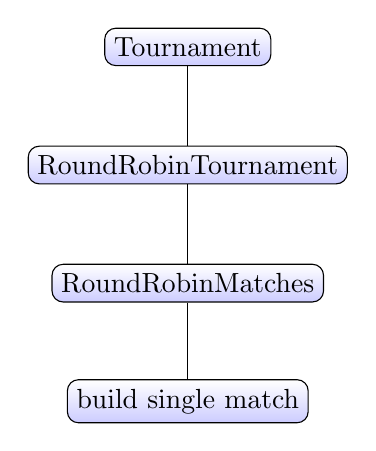
\begin{tikzpicture}[sibling distance=10em,
		every node/.style = {shape=rectangle, rounded corners,
			draw, align=center,
			top color=white, bottom color=blue!20}]]
		\node {Tournament}
		child { node {RoundRobinTournament}
			child { node {RoundRobinMatches}
				child { node {build single match} } }
		};
	\end{tikzpicture}
	\caption{Code structure for a Round Robin tournament}
	\label{fig:round_robin_structure}
\end{figure}

In order to implement a spatial topology tournament a similar approach is
needed. Firstly a new \texttt{Match Generator} class was written.  The
\texttt{SpatialMatches} is a class that generates spatially-structured matches.
In these matches, players interact only with their neighbors rather than the
entire population. According to \cite{Archdeacon1996} graphs can be represented
in many different ways, one of which is by lists of edges.  Due to a various
number of Python packages that are used for graph manipulation,
a more generalized representation of the edges has be selected. Thus edges
are passed as a list argument and \texttt{SpatialMatches} only creates matches
between the
ending nodes of these edges. Finally the class \texttt{SpatialTournament} runs
the spatial tournament. A representation of the code structure now, that the
spatial tournaments have been added, can be seen in
Figure~\ref{fig:spatial_structure}

\begin{figure}
	\centering
	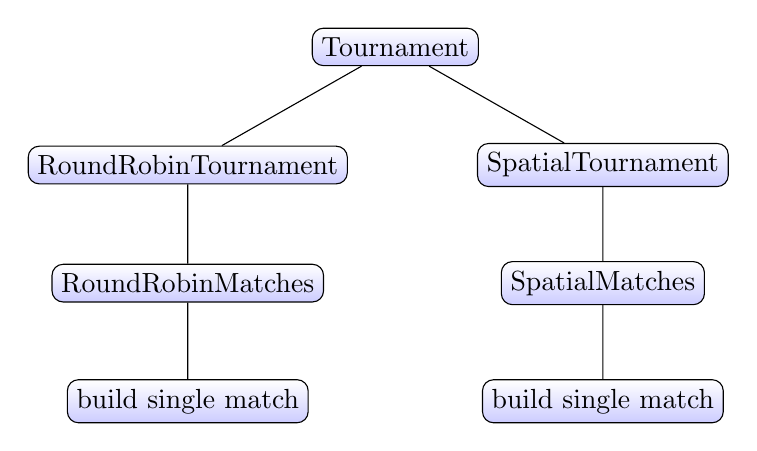
\begin{tikzpicture}[sibling distance=15em,
		every node/.style = {shape=rectangle, rounded corners,
			draw, align=center,
			top color=white, bottom color=blue!20}]]
		\node {Tournament}
		child { node {RoundRobinTournament}
			child { node {RoundRobinMatches}
				child { node {build single match} } }}
		child { node {SpatialTournament}
			child { node {SpatialMatches}
				child { node {build single match} } }
		};
	\end{tikzpicture}
	\caption{Code structure for when Round Robin and Spatial tournaments are
	implemented}
	\label{fig:spatial_structure}
\end{figure}

The Axelrod-Python library is developed using a Test Driven Development (TDD) approach.
All the components are automatically tested using a combination of unit,
property and integration tests (using \url{travis-ci.org}).
Once a new feature is added to the library, a corresponding test must also be
written. The tests are used to ensure compatibility and ensure that the expected
results are returned.
In~\cite{Developer} Percival explains from his personal
experiences the importance of TDD and having tests for every single line of code.
For the spatial tournament a
new unit test have been added. Unit tests are used to invoke a unit of work and
check that the behavior is expected. A unit of work can be any single logical
functional use in the system. In summary, unit tests help to write clean and bug
free code~\cite{Developer}. The unit tests for the \texttt{SpatialTournament} can
be found in Listing~\ref{lst:test_spatial_tournament}.

\begin{listing}[H]
\usemintedstyle{tango}
\begin{minted}
[
frame=lines,
framesep=2mm,
baselinestretch=1.2,
bgcolor=LightBlue,
fontsize=\footnotesize,
linenos
]
{python}
class TestSpatialTournament(unittest.TestCase):

    @classmethod
    def setUpClass(cls):
        cls.game = axelrod.Game()
        cls.players = [s() for s in test_strategies]
        cls.test_name = 'test'
        cls.test_repetitions = test_repetitions
        cls.test_turns = test_turns
        cls.test_edges = test_edges

    def test_init(self):
        tournament = axelrod.SpatialTournament(
            name=self.test_name,
            players=self.players,
            game=self.game,
            turns=self.test_turns,
            edges=self.test_edges,
            noise=0.2)
        self.assertEqual(tournament.match_generator.edges, tournament.edges)
        self.assertEqual(len(tournament.players), len(test_strategies))
        self.assertEqual(tournament.game.score(('C', 'C')), (3, 3))
        self.assertEqual(tournament.turns, 100)
        self.assertEqual(tournament.repetitions, 10)
        self.assertEqual(tournament.name, 'test')
        self.assertTrue(tournament._with_morality)
        self.assertIsInstance(tournament._logger, logging.Logger)
        self.assertEqual(tournament.noise, 0.2)
        anonymous_tournament = axelrod.Tournament(players=self.players)
        self.assertEqual(anonymous_tournament.name, 'axelrod')
\end{minted}
\caption{Source code for TestSpatialTournament class, which is for testing the
         spatial tournaments}
\label{lst:test_spatial_complete_tournament}
\end{listing}

\texttt{TestSpatialTournament} it a simple class for a unit test written for
the spatial tournaments. In Listing~\ref{lst:test_spatial_tournament}, whether
the values of the attributes were passed correctly is being tested. Also whether
the scores are as anticipated. In Listing~\ref{lst:test_spatial_complete_tournament},
another test is shown. Here the results of a spatial tournament on a complete graph
are compared to those of a round robin one.

\begin{listing}[H]
\usemintedstyle{tango}
\begin{minted}
[
frame=lines,
framesep=2mm,
baselinestretch=1.2,
bgcolor=LightBlue,
fontsize=\footnotesize,
linenos
]
{python}
@given(strategies=strategy_lists(strategies=deterministic_strategies,
                                     min_size=2, max_size=2),
           turns=integers(min_value=1, max_value=20))
    def test_complete_tournament(self, strategies, turns):
        """
        A test to check that a spatial tournament on the complete multigraph
        gives the same results as the round robin.
        """
        players = [s() for s in strategies]
        # edges
        edges=[]
        for i in range(0, len(players)) :
            for j in range(i, len(players)) :
                edges.append((i, j))
        # create a round robin tournament
        tournament = axelrod.Tournament(players, turns=turns)
        results = tournament.play()
        # create a complete spatial tournament
        spatial_tournament = axelrod.SpatialTournament(players, turns=turns,
                                                       edges=edges)
        spatial_results =  spatial_tournament.play()
        self.assertEqual(results.ranked_names, spatial_results.ranked_names)
        self.assertEqual(results.nplayers, spatial_results.nplayers)
        self.assertEqual(results.nrepetitions, spatial_results.nrepetitions)
        self.assertEqual(results.payoff_diffs_means,
                                         spatial_results.payoff_diffs_means)
        self.assertEqual(results.payoff_matrix,
                                              spatial_results.payoff_matrix)
        self.assertEqual(results.payoff_stddevs,
                                             spatial_results.payoff_stddevs)
        self.assertEqual(results.payoffs, spatial_results.payoffs)
        self.assertEqual(results.cooperating_rating,
                                         spatial_results.cooperating_rating)
        self.assertEqual(results.cooperation, spatial_results.cooperation)
        self.assertEqual(results.normalised_cooperation,
                                     spatial_results.normalised_cooperation)
        self.assertEqual(results.normalised_scores,
                                          spatial_results.normalised_scores)
        self.assertEqual(results.good_partner_matrix,
                                        spatial_results.good_partner_matrix)
        self.assertEqual(results.good_partner_rating,
					spatial_results.good_partner_rating)
\end{minted}
\caption{Source code for testing a complete spatial tournament}
\label{lst:test_spatial_tournament}
\end{listing}

The source code for the spatial tournaments and the tests can be found
in the Axelrod-Python library. The library is available at
\url{https://github.com/Axelrod-Python},
which is a hosted git repository. This introduces another important aspect
of software development: version control systems (VCS). As stated in \cite{Developer}
TDD and VCS go hand in hand. VCS, is a tool that manages and tracks different
versions of software~\cite{Vogel2014}. Lines of codes are deleted, implementing
errors occur and programmers forgotten. Thus, having the ability to go back to any
given point can be very important. Git is a specific powerful and popular VCS. It
was invented by Linus Torvalds and span to life in April 2005~\cite{Vogel2014}.

The Axelrod-Python library is a project which includes numerous contributors.
Any given addition to the
library has to be submitted by a pull request. Each submission is then
reviewed by members of the core team. This applies to the spatial tournament as well.
In Figure~\ref{fig:github} a conversation containing comments and corrections
can be seen.

O. Campbell and M. Harper are 2 of the 4 core contributors of the library.
Their work, with other contributors, including myself, has had an impact on
the Game Theory community.

In the next section an overview and a summary of the initial experiments
performed is given.

\begin{figure}[H]
	\centering
	\begin{subfigure}[H]{1\textwidth}
		\centering
		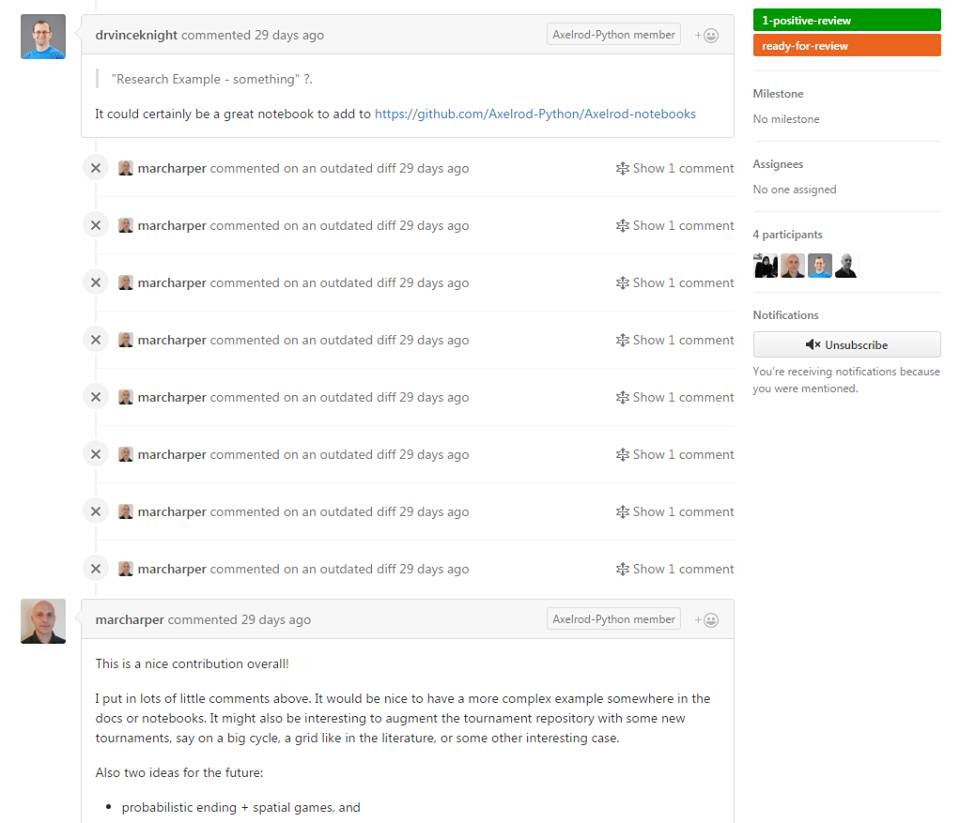
\includegraphics[width=\linewidth]{chapter-three/comments.jpeg}
		\caption{Comments and corrections.}
	\end{subfigure}
	\hfill
	\begin{subfigure}[H]{1\textwidth}
		\centering
		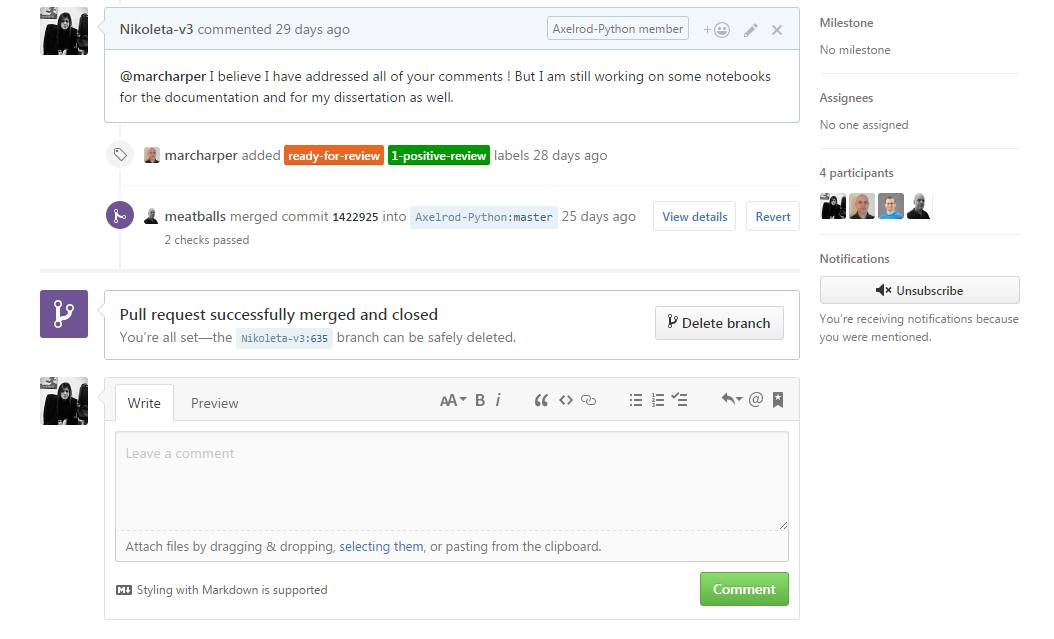
\includegraphics[width=\linewidth]{chapter-three/merging.jpeg}
		\caption{Merging a pull request after reviews.}
	\end{subfigure}
	\caption{On line communication and reviews, through GitHub,
	with members of the Axelrod-Python core team}
	\label{fig:github}
\end{figure}


\subsection{Initial experiment and the three topologies}
In this chapter three simple spatial topologies are considered, all with
deterministic neighborhood size. These will be used to begin to understand how
topology can affect the outcome of tournaments
and which strategies tend to perform well. The three topologies considered are
well represented in the literature~\cite{Axelrod1980a,Szabo2007,Lutz2013}:
\begin{itemize}
	\item A cyclic network: the neighbourhood size is 2.~\cite{Szabo2007}
	\item A periodic lattice: the neighbourhood size is 4.~\cite{Lutz2013}
	\item A complete graph: the neighbourhood size is \(N-1\) (where \(N\) is
	      the number of total strategies. This corresponds to a round robin
	      tournament.~\cite{Axelrod1980a}
\end{itemize}

Figure~\ref{fig:networks}, shows an example of all the aforementioned topologies.

\begin{figure}[!hbtp]
	\centering
	\begin{subfigure}[h]{0.45\textwidth}
		\centering
		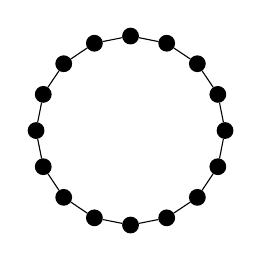
\begin{tikzpicture}[scale=1.2]

   \node (00) [draw, circle, inner sep=2pt,fill] at ( 1.,  0.) {} ;
   \node (01) [draw, circle, inner sep=2pt,fill] at ( 0.92387953,  0.38268343) {} ;
   \node (02) [draw, circle, inner sep=2pt,fill] at ( 0.70710678,  0.70710678) {} ;
   \node (03) [draw, circle, inner sep=2pt,fill] at ( 0.38268343,  0.92387953) {} ;
   \node (04) [draw, circle, inner sep=2pt,fill] at ( 6.12323400e-17,   1.00000000e+00) {} ;
   \node (05) [draw, circle, inner sep=2pt,fill] at (-0.38268343,  0.92387953) {} ;
   \node (06) [draw, circle, inner sep=2pt,fill] at (-0.70710678,  0.70710678) {} ;
   \node (07) [draw, circle, inner sep=2pt,fill] at (-0.92387953,  0.38268343) {} ;
   \node (08) [draw, circle, inner sep=2pt,fill] at (-1.00000000e+00,   1.22464680e-16) {} ;
   \node (09) [draw, circle, inner sep=2pt,fill] at (-0.92387953, -0.38268343) {} ;
   \node (10) [draw, circle, inner sep=2pt,fill] at (-0.70710678, -0.70710678) {};
   \node (11) [draw, circle, inner sep=2pt,fill] at (-0.38268343, -0.92387953) {};
   \node (12) [draw, circle, inner sep=2pt,fill] at (-1.83697020e-16,  -1.00000000e+00) {};
   \node (13) [draw, circle, inner sep=2pt,fill] at ( 0.38268343, -0.92387953) {};
   \node (14) [draw, circle, inner sep=2pt,fill] at ( 0.70710678, -0.70710678) {};
   \node (15) [draw, circle, inner sep=2pt,fill] at ( 0.92387953, -0.38268343) {};

  \draw (15)--(00)--(01)--(02)--(03)--(04)--(05)--(06)--(07)--(08)--(09)--(10)--(11)--(12)--(13)--(14)--(15);
\end{tikzpicture}

		\caption{Cyclic network}
	\end{subfigure}
	\hfill
	\begin{subfigure}[h]{0.52\textwidth}\centering
		\centering
		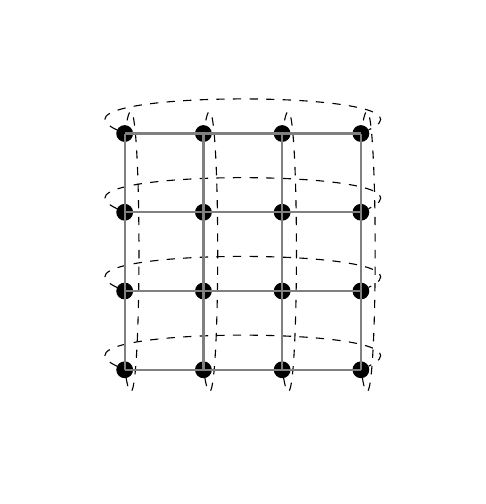
\begin{tikzpicture}

        % First column (tikz has the ability to use loops but I'm drawing it
        % this way so you see how.
        \node (00) [draw, circle, inner sep=2pt,fill] at (0, 0) {};
        \node (01) [draw, circle, inner sep=2pt,fill] at (0, 1) {};
        \node (02) [draw, circle, inner sep=2pt,fill] at (0, 2) {};
        \node (03) [draw, circle, inner sep=2pt,fill] at (0, 3) {};

        % Second column
        \node (10) [draw, circle, inner sep=2pt,fill] at (1, 0) {};
        \node (11) [draw, circle, inner sep=2pt,fill] at (1, 1) {};
        \node (12) [draw, circle, inner sep=2pt,fill] at (1, 2) {};
        \node (13) [draw, circle, inner sep=2pt,fill] at (1, 3) {};

        % Third column
        \node (20) [draw, circle, inner sep=2pt,fill] at (2, 0) {};
        \node (21) [draw, circle, inner sep=2pt,fill] at (2, 1) {};
        \node (22) [draw, circle, inner sep=2pt,fill] at (2, 2) {};
        \node (23) [draw, circle, inner sep=2pt,fill] at (2, 3) {};

        % Fourth column
        \node (30) [draw, circle, inner sep=2pt,fill] at (3, 0) {};
        \node (31) [draw, circle, inner sep=2pt,fill] at (3, 1) {};
        \node (32) [draw, circle, inner sep=2pt,fill] at (3, 2) {};
        \node (33) [draw, circle, inner sep=2pt,fill] at (3, 3) {};


        % I am drawing the periodic boundaries before the rest of the grid
        % so that they appear 'behind' the rest of the images.
        % Draw the period horizontal boundary
        \draw[dashed] (00) to[out=155,in=25 ] (30);
        \draw[dashed] (01) to[out=155,in=25 ] (31);
        \draw[dashed] (02) to[out=155,in=25 ] (32);
        \draw[dashed] (03) to[out=155,in=25 ] (33);

        % Draw the period vertical boundary
        \draw[dashed] (00) to[out=-80,in=80] (03);
        \draw[dashed] (10) to[out=-80,in=80] (13);
        \draw[dashed] (20) to[out=-80,in=80] (23);
        \draw[dashed] (30) to[out=-80,in=80] (33);

        % Draw a grid (this is a tikz shortcut)
        \draw[style=help lines,thick] (0,0) grid  (3,3);
\end{tikzpicture}

		\caption{Periodic lattice with degree 4 network}
	\end{subfigure}
	\hfill
	\begin{subfigure}[h]{0.52\textwidth}\centering
		\centering
		\begin{tikzpicture}
  \graph {subgraph K_n [n=8,clockwise, nodes={draw, circle, fill=black, scale=0.7}, empty nodes,radius=2cm]};
\end{tikzpicture}

		\caption{A complete or round robin network}
	\end{subfigure}
	\caption{Network topologies}
	\label{fig:networks}
\end{figure}

For each topology, a fixed number of strategies out of the 132 of Axelrod-Python
library (1.7.0) are chosen randomly. The number of strategies define the size of the
tournament. In the following experiments, the tournament size can be either
5 or 50. In~\autoref{chap:Four} a more expansive tournament size range is
considered for the corresponding analysis.

Subsequently, the strategies are allocated on the graph, based
on the topology, and they compete with their neighbors in a IPD tournament.
For the cyclic and lattice topology, once the first game is complete,
the strategies are randomly shuffled and allocated on the graph again. This aims
to ensure that their particular position on the network is taken in to account.
This shuffle is repeated 10 times. The selection of strategies is repeated 100 times
and each tournament of an IPD consists of 200 turns and 10 repetitions.
Algorithm~\ref{simple-experiment-rules} illustrates these rules.

\begin{algorithm}
	\caption{Simple Experiments Rules}\label{simple-experiment-rules}
	\begin{algorithmic}
		\Procedure{Running Experiment}{}
		\BState \emph{loop}:
		\For {$\textit{i} \gets \textit{ 0 to 100}$}
		\State $seed$ \Comment{by setting a seed here, the program allows the reproduction
		of the same players list, for each experiment}
		\State $player \gets \textit{random.strategies}$.
		\For {$i \gets \textit{0 to 10}$}
		\State $G \gets \textit{create.graph}$.
		\State $edges \gets \textit{G.egdes}$
		\State $results \gets \textit{play.tournament}$.
		\emph{loop}.
		\EndFor
		\EndFor
		\EndProcedure
	\end{algorithmic}
\end{algorithm}

In the next section, preliminary analysis of the experiments aforementioned
is described. Followed by, an in depth analysis in~\autoref{sub:analyzing_the_effect_of_the_topologies}.
There, the concept of winning ratio and normalized average score are introduced.
Finally, the results have been summarized in~\autoref{sub:summary}, offering further
avenues of research.

\subsection{Initial Analysis}
\label{sub:initial_analysis}
Hereafter, various strategies from the Axelrod-Python library have been referenced.
Though for some a brief explanation is given, describing all 132, would be
unreasonable. Therefore a table containing all strategies and their explanation
(as documented by the Axelrod-Python library), can be found in the Appendix~\ref{append:strategies}.
For each of the tournaments run, the following parameters are recorded:

\begin{multicols}{3}
	\begin{itemize}
		\item players list
		\item seed
		\item parameter
		\item player index
		\item player name
		\item cooperating ratio
		\item degree
		\item neighbors
		\item neighborhood size
		\item ranking
		\item scores
		\item normalized scores
		\item average score
		\item R
		\item P
		\item S
		\item T
		\item connectivity
		\item clustering
		\item cliques
		\item neighbors scores
		\item normalized neighbors score
		\item normalized average neighborhood score
	\end{itemize}
\end{multicols}

This section will describe the findings of a basic statistical analysis of these
records.

In the experiments, in which the topology is that of a round robin,
100 different tournaments have been recorded.
For the other experiments, for both tournament sizes (5 and 50),
1000 tournaments have been played. Containing 100 different strategy sets, each of
which play 10 tournaments.

Moreover, for the cyclic experiments as shown in Table~\ref{sum-cicle}, the degree is
and the payoffs are fixed for both tournament sizes. For tournaments of size 5,
the mean average score is 2.45, with a minimum value of 0.0175 (Bully) and a maximum
value of 4.95 (Anti Tit For Tat). The mean average score of the neighbors score
is 2.45 with a standard deviation of 0.55.
The mean average score does not seem to differ for size equal to 50, which is at
2.39. Though, in the experiment with a size of fifty a strategy
achieved an average score of 0 ($phi$). The maximum average score is equal to
5 (Meta Minority). Additionally the average score of the neighbors ranges
from 0.05 to 4.71. Concerning the graph measures, as explained in ~\autoref{sub:graph-theory},
clustering coefficient is zero and connectivity fixed to 2.

\begin{table}[!hbtp]
	\centering
	\begin{adjustbox}{width=1\textwidth, height=0.15\textwidth}
		\small
		\begin{tabular}{cccccccccc}
				\toprule
			Cyclic & \multicolumn{3}{|c|}{tournament size 5 and 50} & \multicolumn{3}{c|}{tournament size 5} & \multicolumn{3}{c}{tournament size 50}                             \\\midrule

			     & (R,P,S,T) & degree & connectivity & average score & average neighbors score & clustering & average score & average neighbors score & clustering \\\midrule
			mean & (3,1,0,5) & 2.0    & 2.0          & 2.45          & 2.45                    & 0.00       & 2.39          & 2.39                    & 0.00       \\\midrule
			std  & (0,0,0,0) & 0.0    & 0.0          & 0.74          & 0.55                    & 0.00       & 0.77          & 0.57                    & 0.00       \\\midrule
			min  & (3,1,0,5) & 2.0    & 2.0          & 0.01          & 0.35                    & 0.00       & 0.00          & 0.05                    & 0.00       \\\midrule
			max  & (3,1,0,5) & 2.0    & 2.0          & 4.95          & 4.39                    & 0.00       & 5.00          & 4.71                    & 0.00       \\ \bottomrule
		\end{tabular}
	\end{adjustbox}
	\caption{Summary table for topology circle}
	\label{sum-cicle}
\end{table}

For the lattice topologies, a table that summarizes the data is shown in Table
~\ref{sum-lattice}. For both size values the payoffs are the same (\(R=3, P=1,
S=0, T=5\)) and the degree is fixed at 4. For size 5 the average score
varies between 0.52 (Cycler CCD) and 4.24 ($pi$). The average score of the neighbors
varies between 1.32 and 3.15. Much higher, compared to both the cyclic experiments.
This is understood to be based on the fact that the number of neighbors is now
doubled. For size 50, the mean average score is 2.39 and the mean average neighbor
score 2.39. The maximum average score was achieved by Fortress3, 4.97 and the
minimum, 0.01, by strategy $e$. The clustering coefficient is 1 and for size
50 is 0.5. This shows that in the lattice example the strategies tend to create
groups, complete subgraphs.

\begin{table}[!hbtp]
	\centering
	\begin{adjustbox}{width=1\textwidth, height=0.15\textwidth}
		\small
		\begin{tabular}{cccccccccc}
				\toprule
			Lattice & \multicolumn{3}{|c|}{tournament size 5 and 50} & \multicolumn{3}{c|}{tournament size 5} & \multicolumn{3}{c}{tournament size 50}                            \\ \midrule
			     & (R,P,S,T) & degree & connectivity & average score & average neighbors score & clustering & average score & average neighbors score & clustering \\ \midrule
			mean & (3,1,0,5) & 4.0    & 4.0          & 2.45          & 2.44                    & 1.0        & 2.39          & 2.39                    & 0.5        \\ \midrule
			std  & (0,0,0,0) & 0.0    & 0.0          & 0.57          & 0.36                    & 0.0        & 0.59          & 0.33                    & 0.00       \\ \midrule
			min  & (3,1,0,5) & 4.0    & 4.0          & 0.52          & 1.32                    & 1.0        & 0.01          & 1.04                    & 0.5        \\ \midrule
			max  & (3,1,0,5) & 4.0    & 4.0          & 4.24          & 3.15                    & 1.0        & 4.97          & 3.61                    & 0.5        \\ \bottomrule
		\end{tabular}
	\end{adjustbox}
	\caption{Summary table for the lattice topology}
	\label{sum-lattice}
\end{table}

Finally, for the round robin tournaments, 100 tournaments were performed for both
sizes. Parameters such as neighborhood size and neighbor's score
were not computed for the round robin topology. This is because all players
interact with each other thus there were not any additional information to be
gained. In Table~\ref{sum-rr}, the average score the strategies achieved
in this topology for both sizes is shown. In a tournament of size 50, the mean average
score is 2.39 with a standard deviation of 0.335.

\begin{table}[H]
	\centering
	\begin{adjustbox}{width=0.5\textwidth,height=0.15\textwidth}
		\small
		\begin{tabular}{ccccc}
				\toprule
		Round Robin & \multicolumn{1}{|c|}{tournament size 5} & \multicolumn{1}{c}{tournament size 50} \\ \hline

		            & average score                          & average score                           \\ \hline
		mean        & 2.44                                   & 2.39                                    \\ \hline
		std         & 0.57                                   & 0.33                                    \\ \hline
		min         & 0.52                                   & 1.52                                    \\ \hline
		max         & 4.24                                   & 3.33                                    \\ \bottomrule
	\end{tabular}
\end{adjustbox}
	\caption{Summary table for round robin topology}
	\label{sum-rr}
\end{table}

In this section the structure of the source code for implementing the spatial
tournament, by adding to the Axelrod-Python library was analyzed. Furthermore,
using the verified code, various experiments were conducted with different
topologies
and number of players participating in each tournament. An overview of the
data sets produced was done but now in the following sections
some more analysis on the results will be performed that aim to understand
the performance of the strategies.

\section{Analyzing the effect of the topologies}
\label{sub:analyzing_the_effect_of_the_topologies}
In the data all 132 strategies of Axelrod-Python library have participated in at
least one tournament. Not all strategies participated in an equal number of tournaments.
Forcing the strategies to perform in a uniform number is
not an option because the random effect is needed for validation of the
results. For a measure of
performance, instead of using the number of tournaments won, the analysis will
be using the ratio of wins in~\autoref{sub:winning_ratio}.
The winning ratio is defined as the number of tournaments a strategy was ranked
first divided by the number of tournaments the strategy competed in.
Additionally, the normalized average score each strategy
achieved will also be studied in~\autoref{sub:normalized_av_score}.
Lastly in~\autoref{sub:regression}, a regression model is considered to
attempt to identify the important factors relevant to performance in various
topologies.

\subsection{Winning Ratio}
\label{sub:winning_ratio}
In the experiment where the strategies compete on a cyclic network, 124 strategies
out of the 132 have a winning ratio greater than zero. In other words, 8 strategies
won no tournaments. These strategies are shown in Table~\ref{winning-ratio-zero-cyclic-five}:

\begin{table}[h]
	\centering
	\begin{adjustbox}{width=1\textwidth}
		\small
		\begin{tabular}{@{}|l|l|l|l|l|l|l|l|l|l|@{}}
			\hline
			\textbf{Strategies list}     & \multicolumn{1}{c|}{\textbf{Description}}                                                                                     \\ \hline
			ALLCorALLD          & Simply repeats its last move, and so mimics ALLC or ALLD after round one.                                            \\ \hline
			Tricky Cooperator   & Almost always cooperates, but will try to trick the opponent by defecting.                                           \\ \hline
			ThueMorseInverse    & Defects or cooperates according to the Thue-Morse sequence (Inverse of ThueMorse).                                   \\ \hline
			SolutionB5          & A finite state machine strategy, described in~\cite{Ashlock2015}  																									 \\ \hline
			Hard Tit For 2 Tats & A variant of Tit For Two Tats that uses a longer history for retaliation.                                            \\ \hline
			BackStabber         & Forgives the first 3 defections but on the fourth,will defect forever. Defects on the last 2 rounds unconditionally. \\ \hline
			Prober              & Plays D, D, C, C initially. Defects forever if opponent cooperated in moves 2 and 3. Otherwise plays TFT.            \\ \hline
			Cycler DDC          & A player that repeats the sequence DDC indefinitely.                                                                 \\ \hline
		\end{tabular}
	\end{adjustbox}
	\caption{Strategies with winning ratio 0 in the cyclic experiment with tournament
	size 5}
	\label{winning-ratio-zero-cyclic-five}
\end{table}

In the lattice topology as well, 8 strategies do not have a non-zero winning ratio.
Among them Tricky Cooperator, Cycle DDC and AllCorAllD again. The rest of the
strategies and a simple explanation of them can be found in Table~\ref{winning-ratio-zero-lattice-five}.

\begin{table}[h]
	\centering
	\begin{adjustbox}{width=1\textwidth}
		\small
		\centering
		\begin{tabular}{|l|l|}
			\hline
			\textbf{Strategies list}     & \multicolumn{1}{c|}{\textbf{Description}}                                                                             \\ \hline
			Bully                   & A player that behaves opposite to Tit For Tat, including first move.                                          \\ \hline
			Fortress4               & A finite state machine player~\cite{Moore1977}                                                                \\ \hline
			Hard Go By Majority: 5  & \begin{tabular}[c]{@{}l@{}}A player examines the history of the opponent: if the opponent has more defections \\ than cooperations then the player defects. Here the player has a memory of 5.\end{tabular}                                            \\ \hline
			Hard Go By Majority: 40 & A Hard Go By Majority player, with memory 40.                                                                 \\ \hline
			Sneaky Tit For Tat      & Tries defecting once and repents if punished.                                                                 \\ \hline
		\end{tabular}
	\end{adjustbox}
	\caption{Strategies with winning ratio 0 in the periodic lattice experiment with
	tournament size 5}
	\label{winning-ratio-zero-lattice-five}
\end{table}

In the round robin tournament 61 strategies ranked a winning ratio of zero.
Among them Cycler CCD, Tricky Cooperator, Fortress4, Bully, and the Majority
strategies.

On the other hand the strategies with the highest winning ratio for each
topology are as follows:

\begin{itemize}
	\item Cyclic topology with a winning ratio of 0.56 ZD-GEN-2, followed by Punisher
	      with 0.55 and Soft Grudger with 0.53
	\item Lattice topology with a ratio of 0.45 BackStabber and Meta Majority
	      Memory one. Followed by Cycler CCD with 0.44, Limited Retaliate(0.05/20)
	      and Stochastic WSLS with 0.43 winning ratio
	\item Round Robin topology with a winning ratio of 1 : Raider, Gradual, Limited
	      Retaliate(0.05/20) and BackStabber
\end{itemize}

In every topology the highest ranking strategy is different.
Only BackStabber seems to be repeated, even so in the cyclic
topology it had a winning ratio of zero. BackStabber is one of highest ranking
strategies in the overall round robin tournament performed by the Axelrod-Python
library. ALLCorALLD, Cycler CCD, Tricky Cooperator and Bully did badly in all
three topologies.

When considering tournaments of size 50 no strategies have a zero ratio
(in any topology). The number of tournaments participated in tournament size 5
ranges from 10 to 90, where in the tournament size 50 from 270 to 570. The higher
the number of tournaments participated the higher probabilities of winning at
least one. This could explain the existence of only non zero winning ratios.

The strategies with the highest winning ratio for each respective topologies are
as follow:

\begin{itemize}
	\item Cyclic topology with a winning ratio of 0.038 Soft Go By Majority:10.
	      Followed by Nice Average Copier with 0.037 and \(e\) with 0.036. Raider
	      has the fourth higher winning ratio on 0.034
	\item Lattice topology with a winning ratio of 0.037 Adapative Pavlov 2006.
	      Followed by Fool Me Once with 0.036 and Raider with 0.035. Inverse
	      Punisher had a winning ratio of 0.033, the fourth highest of all
	\item Round Robin topology with a winning ratio of 0.86 PSO Gambler, followed
	      by EvolvedLookerUp with 0.60
\end{itemize}

In the cyclic and periodic lattice topology the highest winning ratio achieved
was 0.038. The number is lower than any other experiment due to the range of
tournaments participated. In the round robin experiment the maximum number of
participations was 57, explaining the big difference in the winning ratio between
these experiments. PSO Gambler that achieved the highest ratio is also the current
winner of the Axelrod-Python tournament~\cite{pso_gambler}.

Overall, for the results of all six experiments no similarities stick out.
A more appropriate visualization of the top ranking strategies for both
sizes are shown in Figures~\ref{fig:winning-rankings-five-c-l}~\ref{fig:winning-rankings-five-c-r}
~\ref{fig:winning-rankings-five-l-r} and Figures~\ref{fig:winning-rankings-fifty-c-l}
~\ref{fig:winning-rankings-fifty-c-r}~\ref{fig:winning-rankings-fifty-l-r}.
The line graph shows the rank change for each strategy over two topologies.
This will improve the understanding on the correlation of the top ranking strategies.
For experiments of tournament size 5, 3
pairs for the experiments are illustrated. Overall, the strategies with an
average good ranking in all experiments were Punisher, Raider and BackStabber.
A similarly approach for experiments of size 50.
The overall successful strategies are Nice Average Copier, Raider and Fool Me Once.

Raider is a repeatedly successful strategies for more than one experiment.
It is a finite state machine strategy found in~\cite{DBLP:conf/foci/AshlockTA14}.
For now Raider strategy seems to be a well performed strategy for any
given random situation.

Illustration of the ratios for each experiment in ascending order can be found
in Appendix~\ref{append:wining-ratio-further-plot},
Figure~\ref{fig:winning-fifty} and Figure~\ref{fig:winning-five}.

\begin{figure}[H]
	\centering
	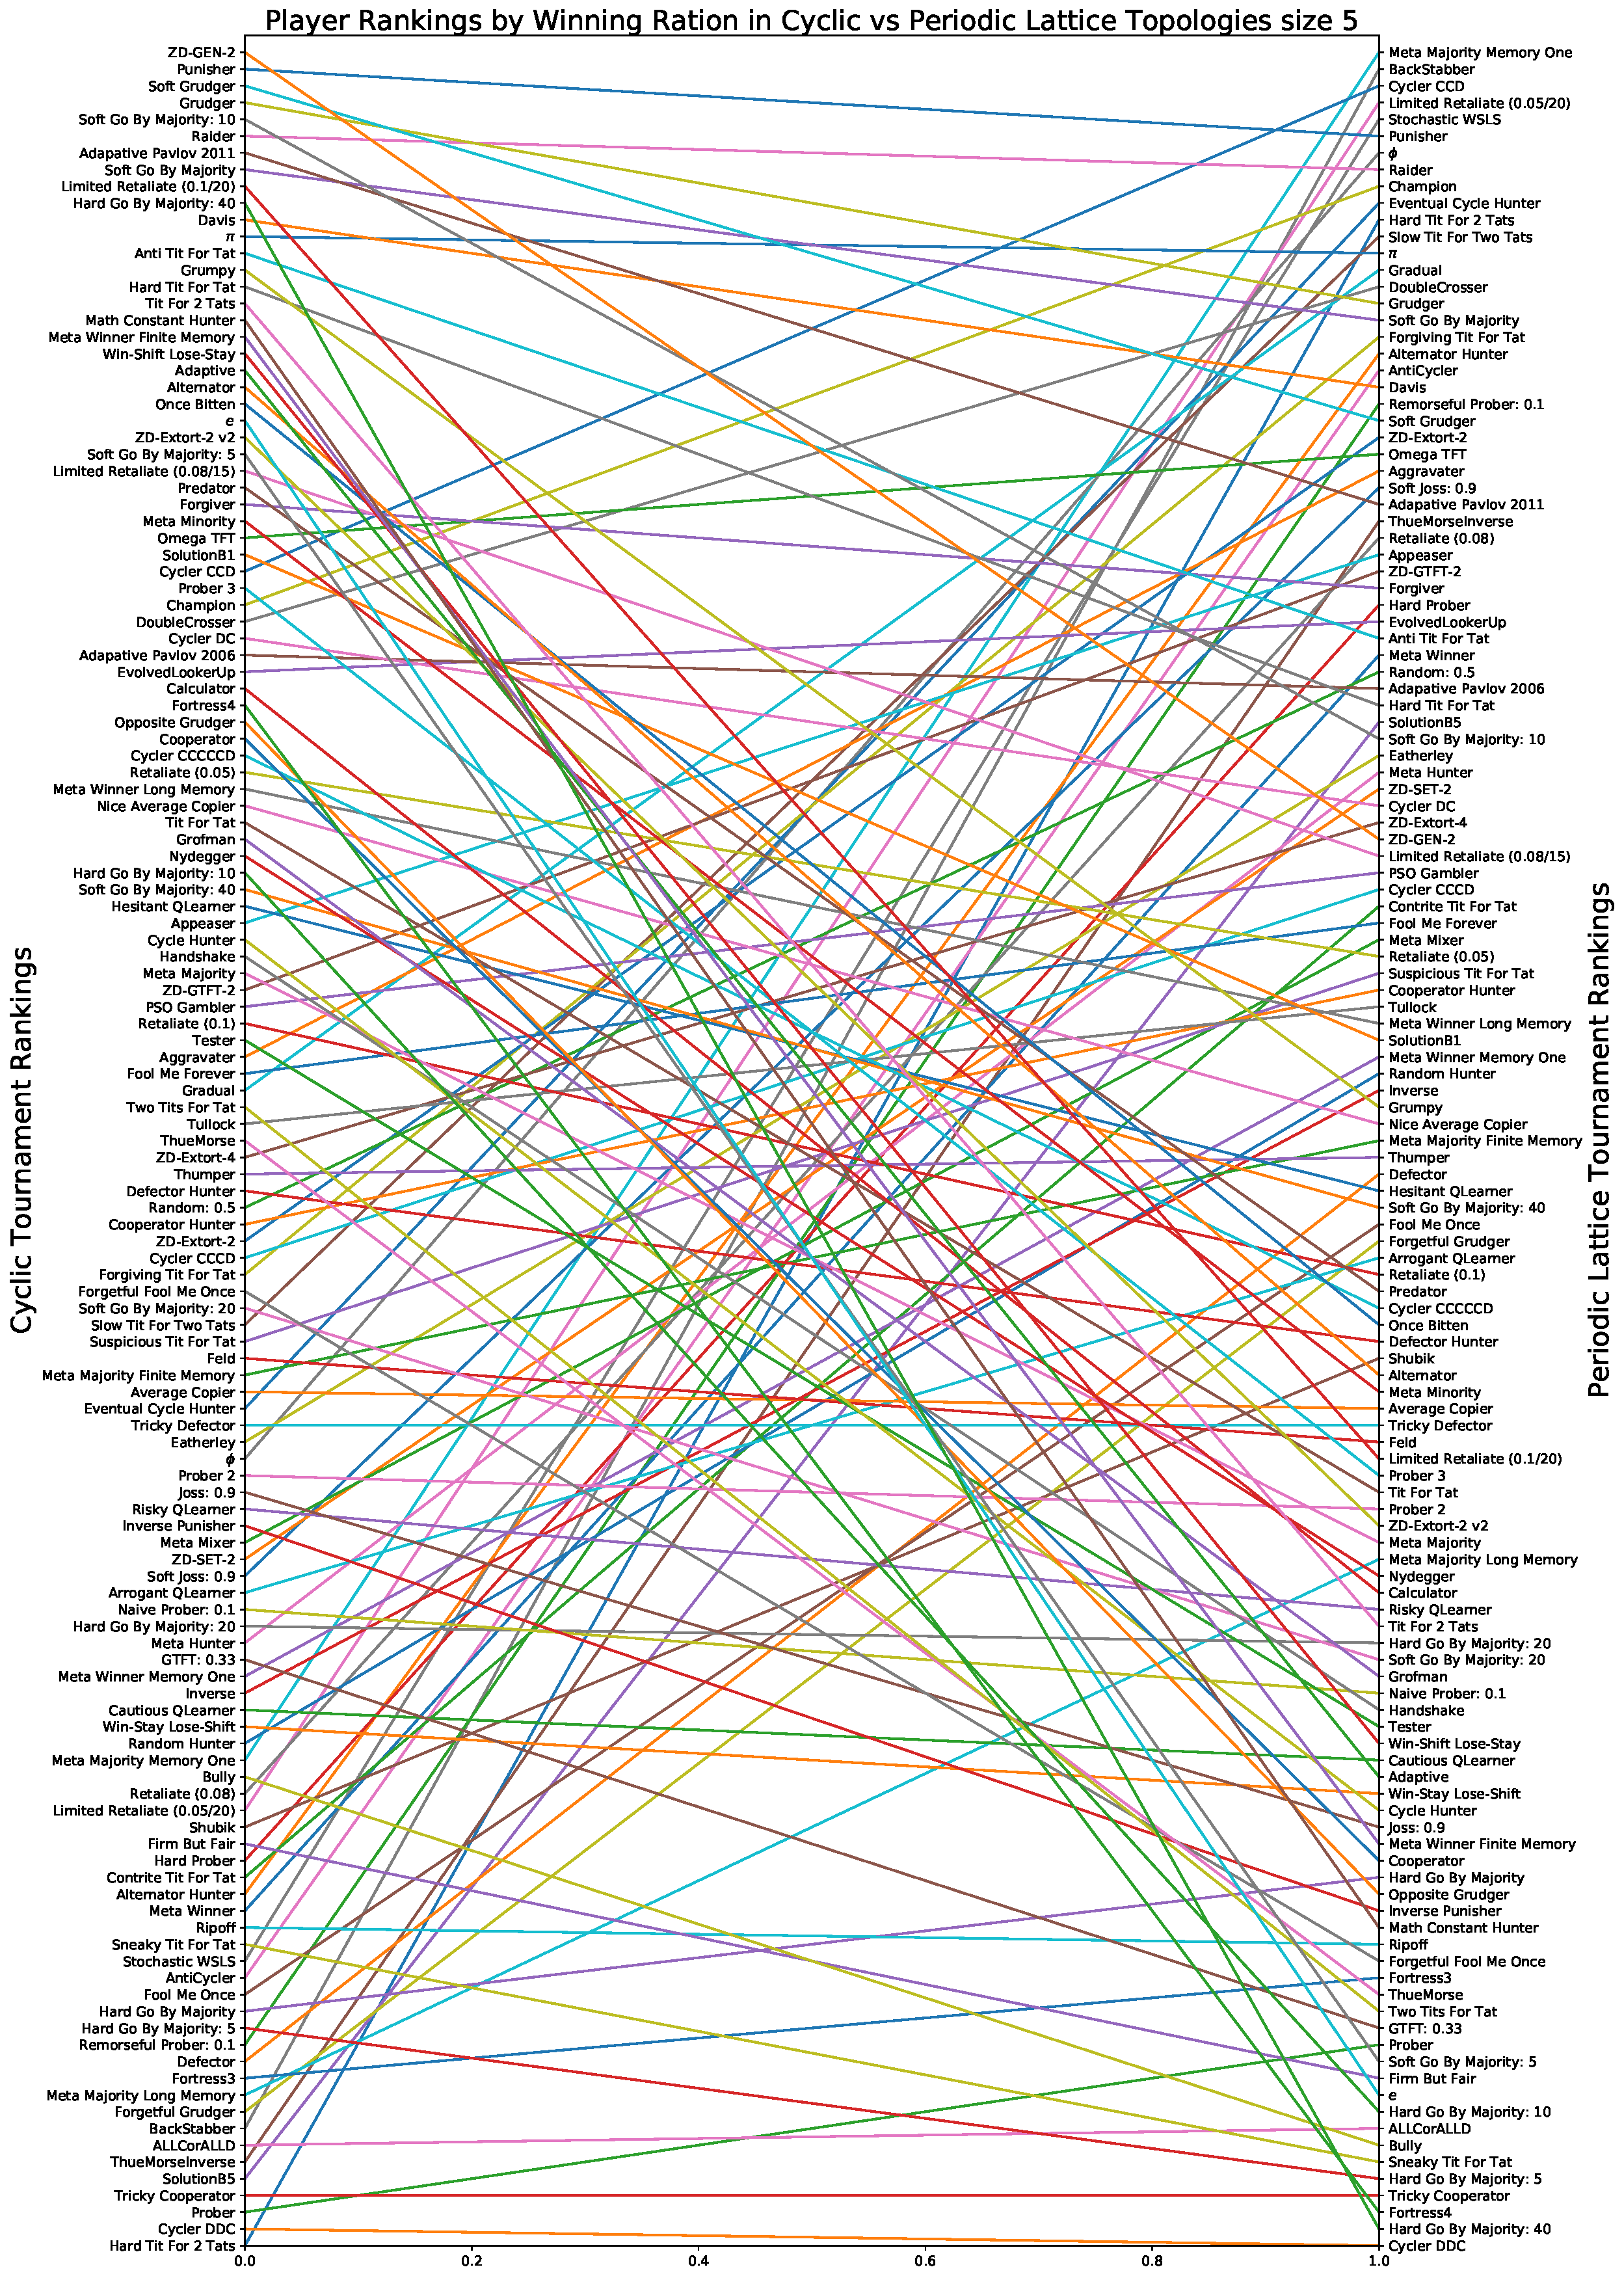
\includegraphics[width=\linewidth]{chapter-three/lines-cyclic-lattice-5.pdf}
	\caption{Cyclic vs Periodic Lattice topologies size 5}
	\label{fig:winning-rankings-five-c-l}
\end{figure}

\begin{figure}[H]
	\centering
	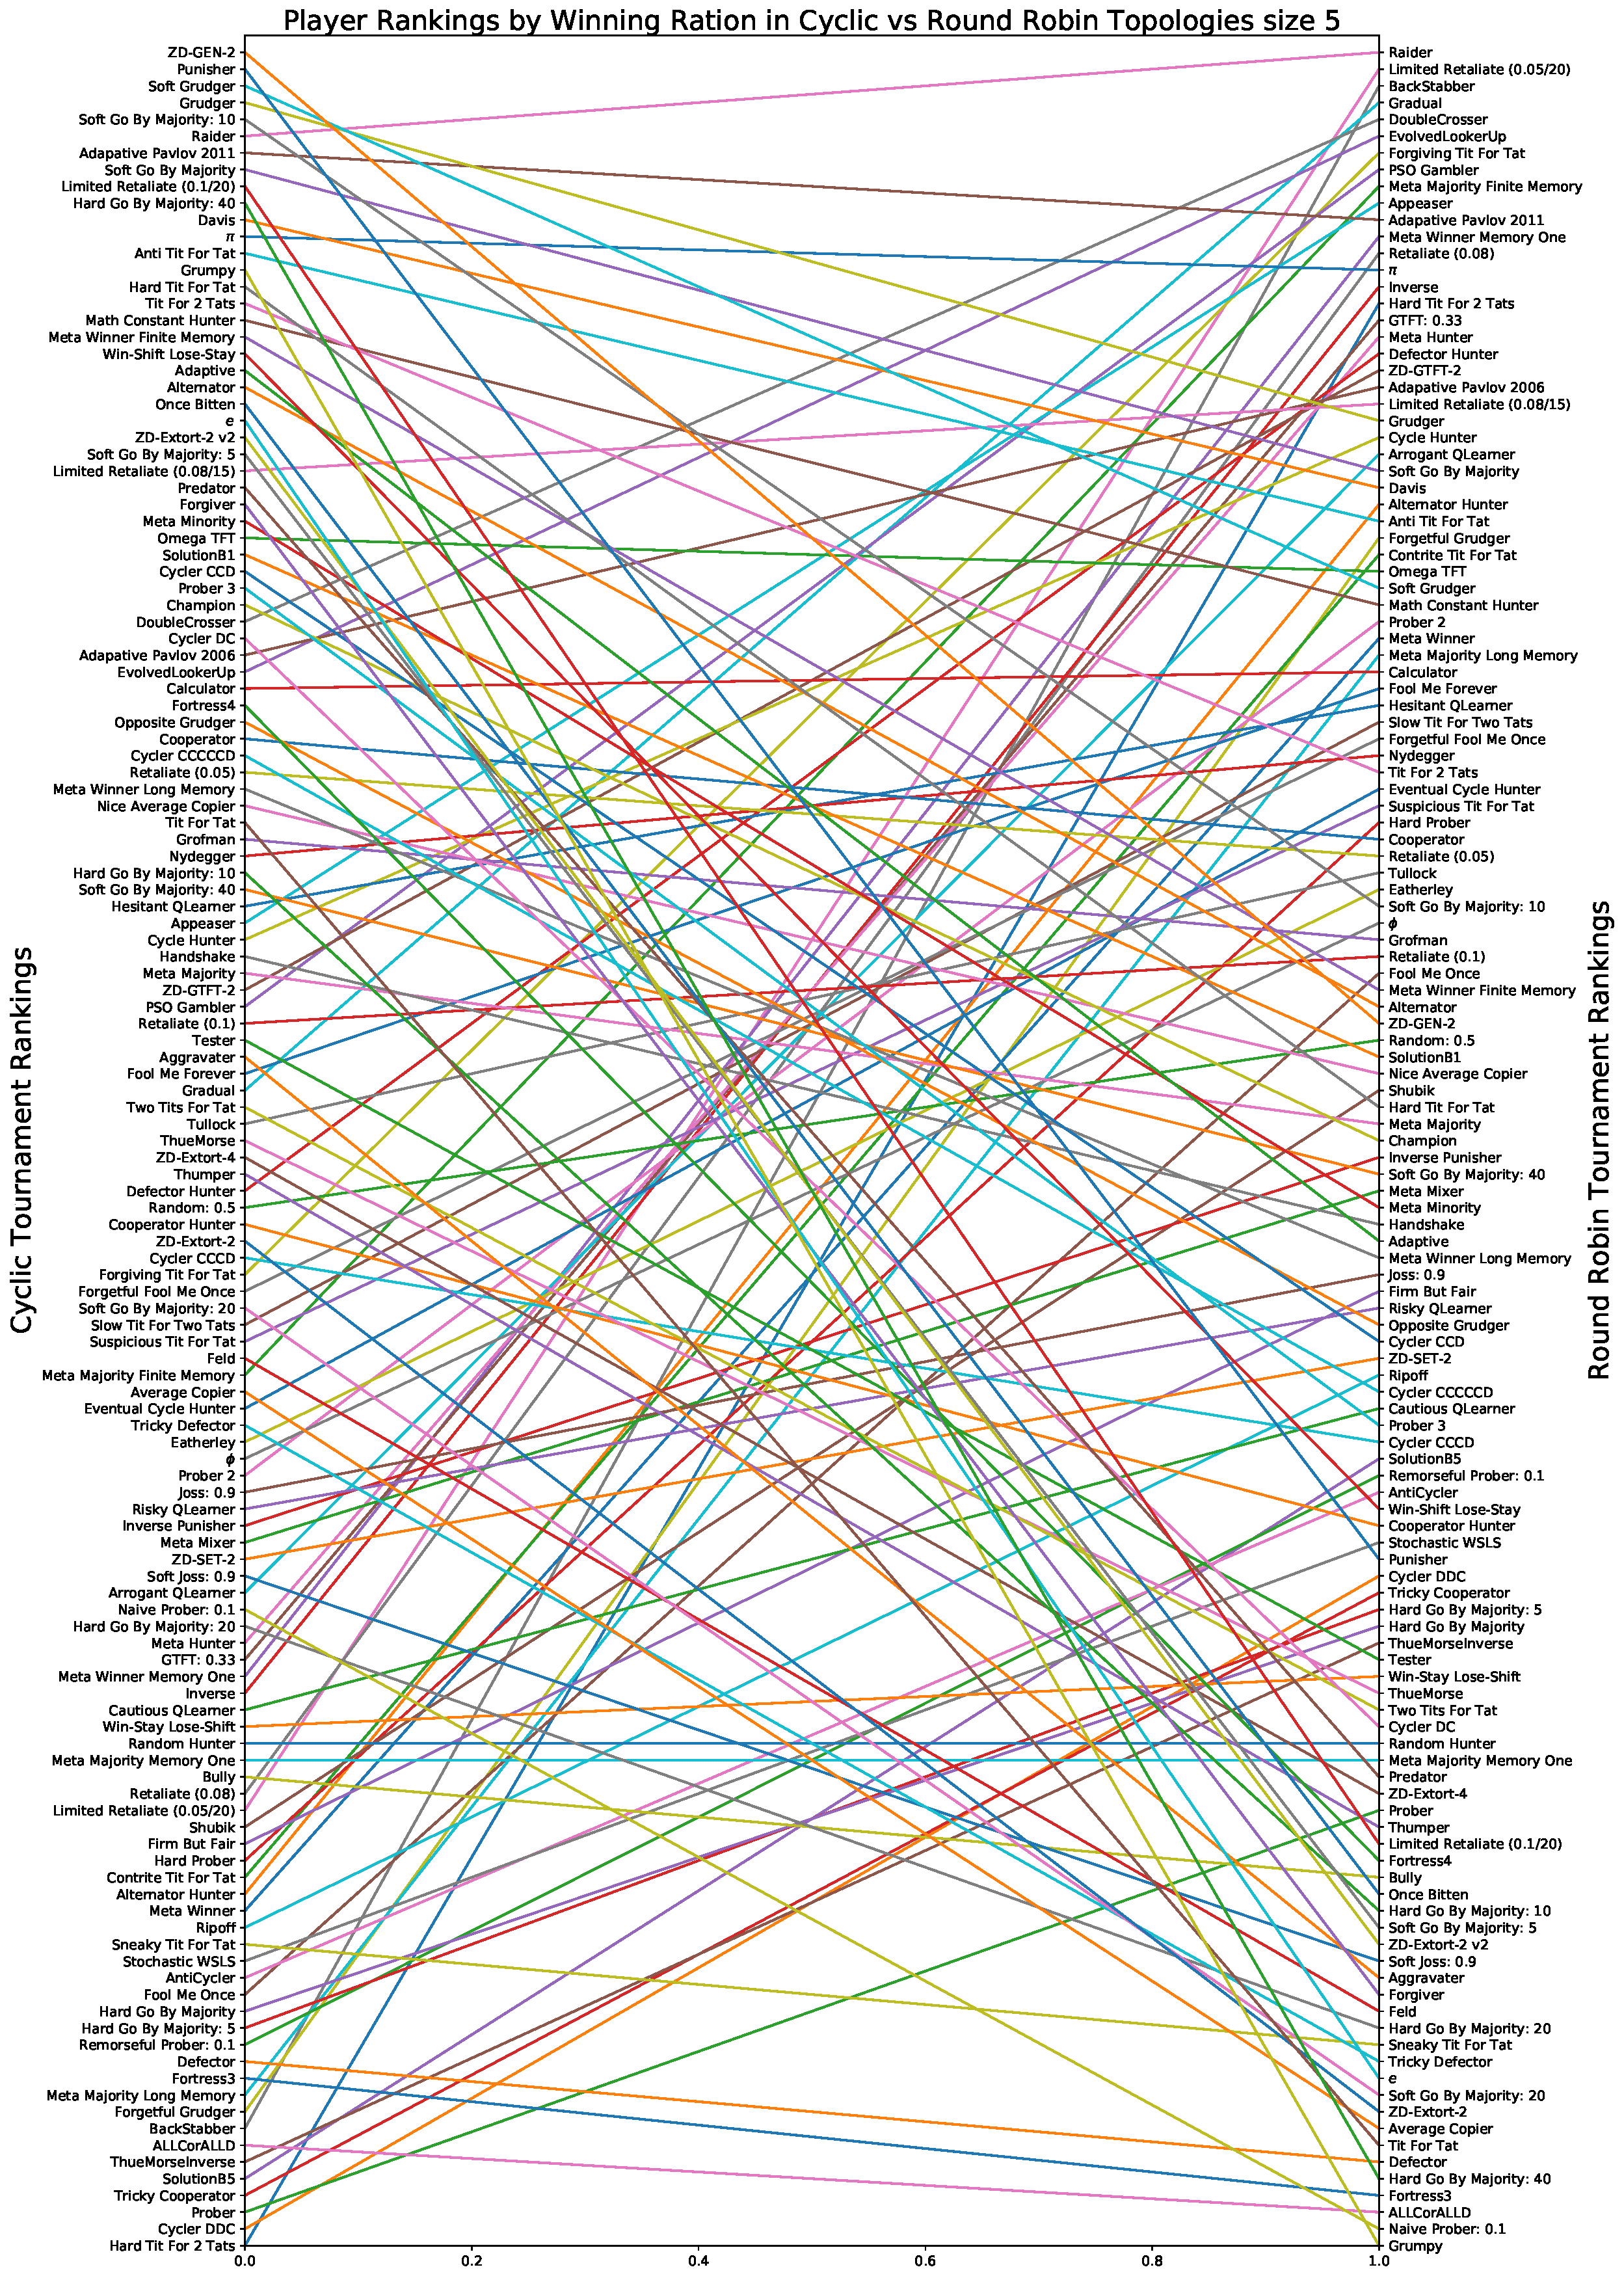
\includegraphics[width=\linewidth]{chapter-three/lines-cyclic-round-robin-5.pdf}\
	\caption{Cyclic vs Round Robin topologies size 5}
	\label{fig:winning-rankings-five-c-r}
\end{figure}

\begin{figure}[H]
	\centering
	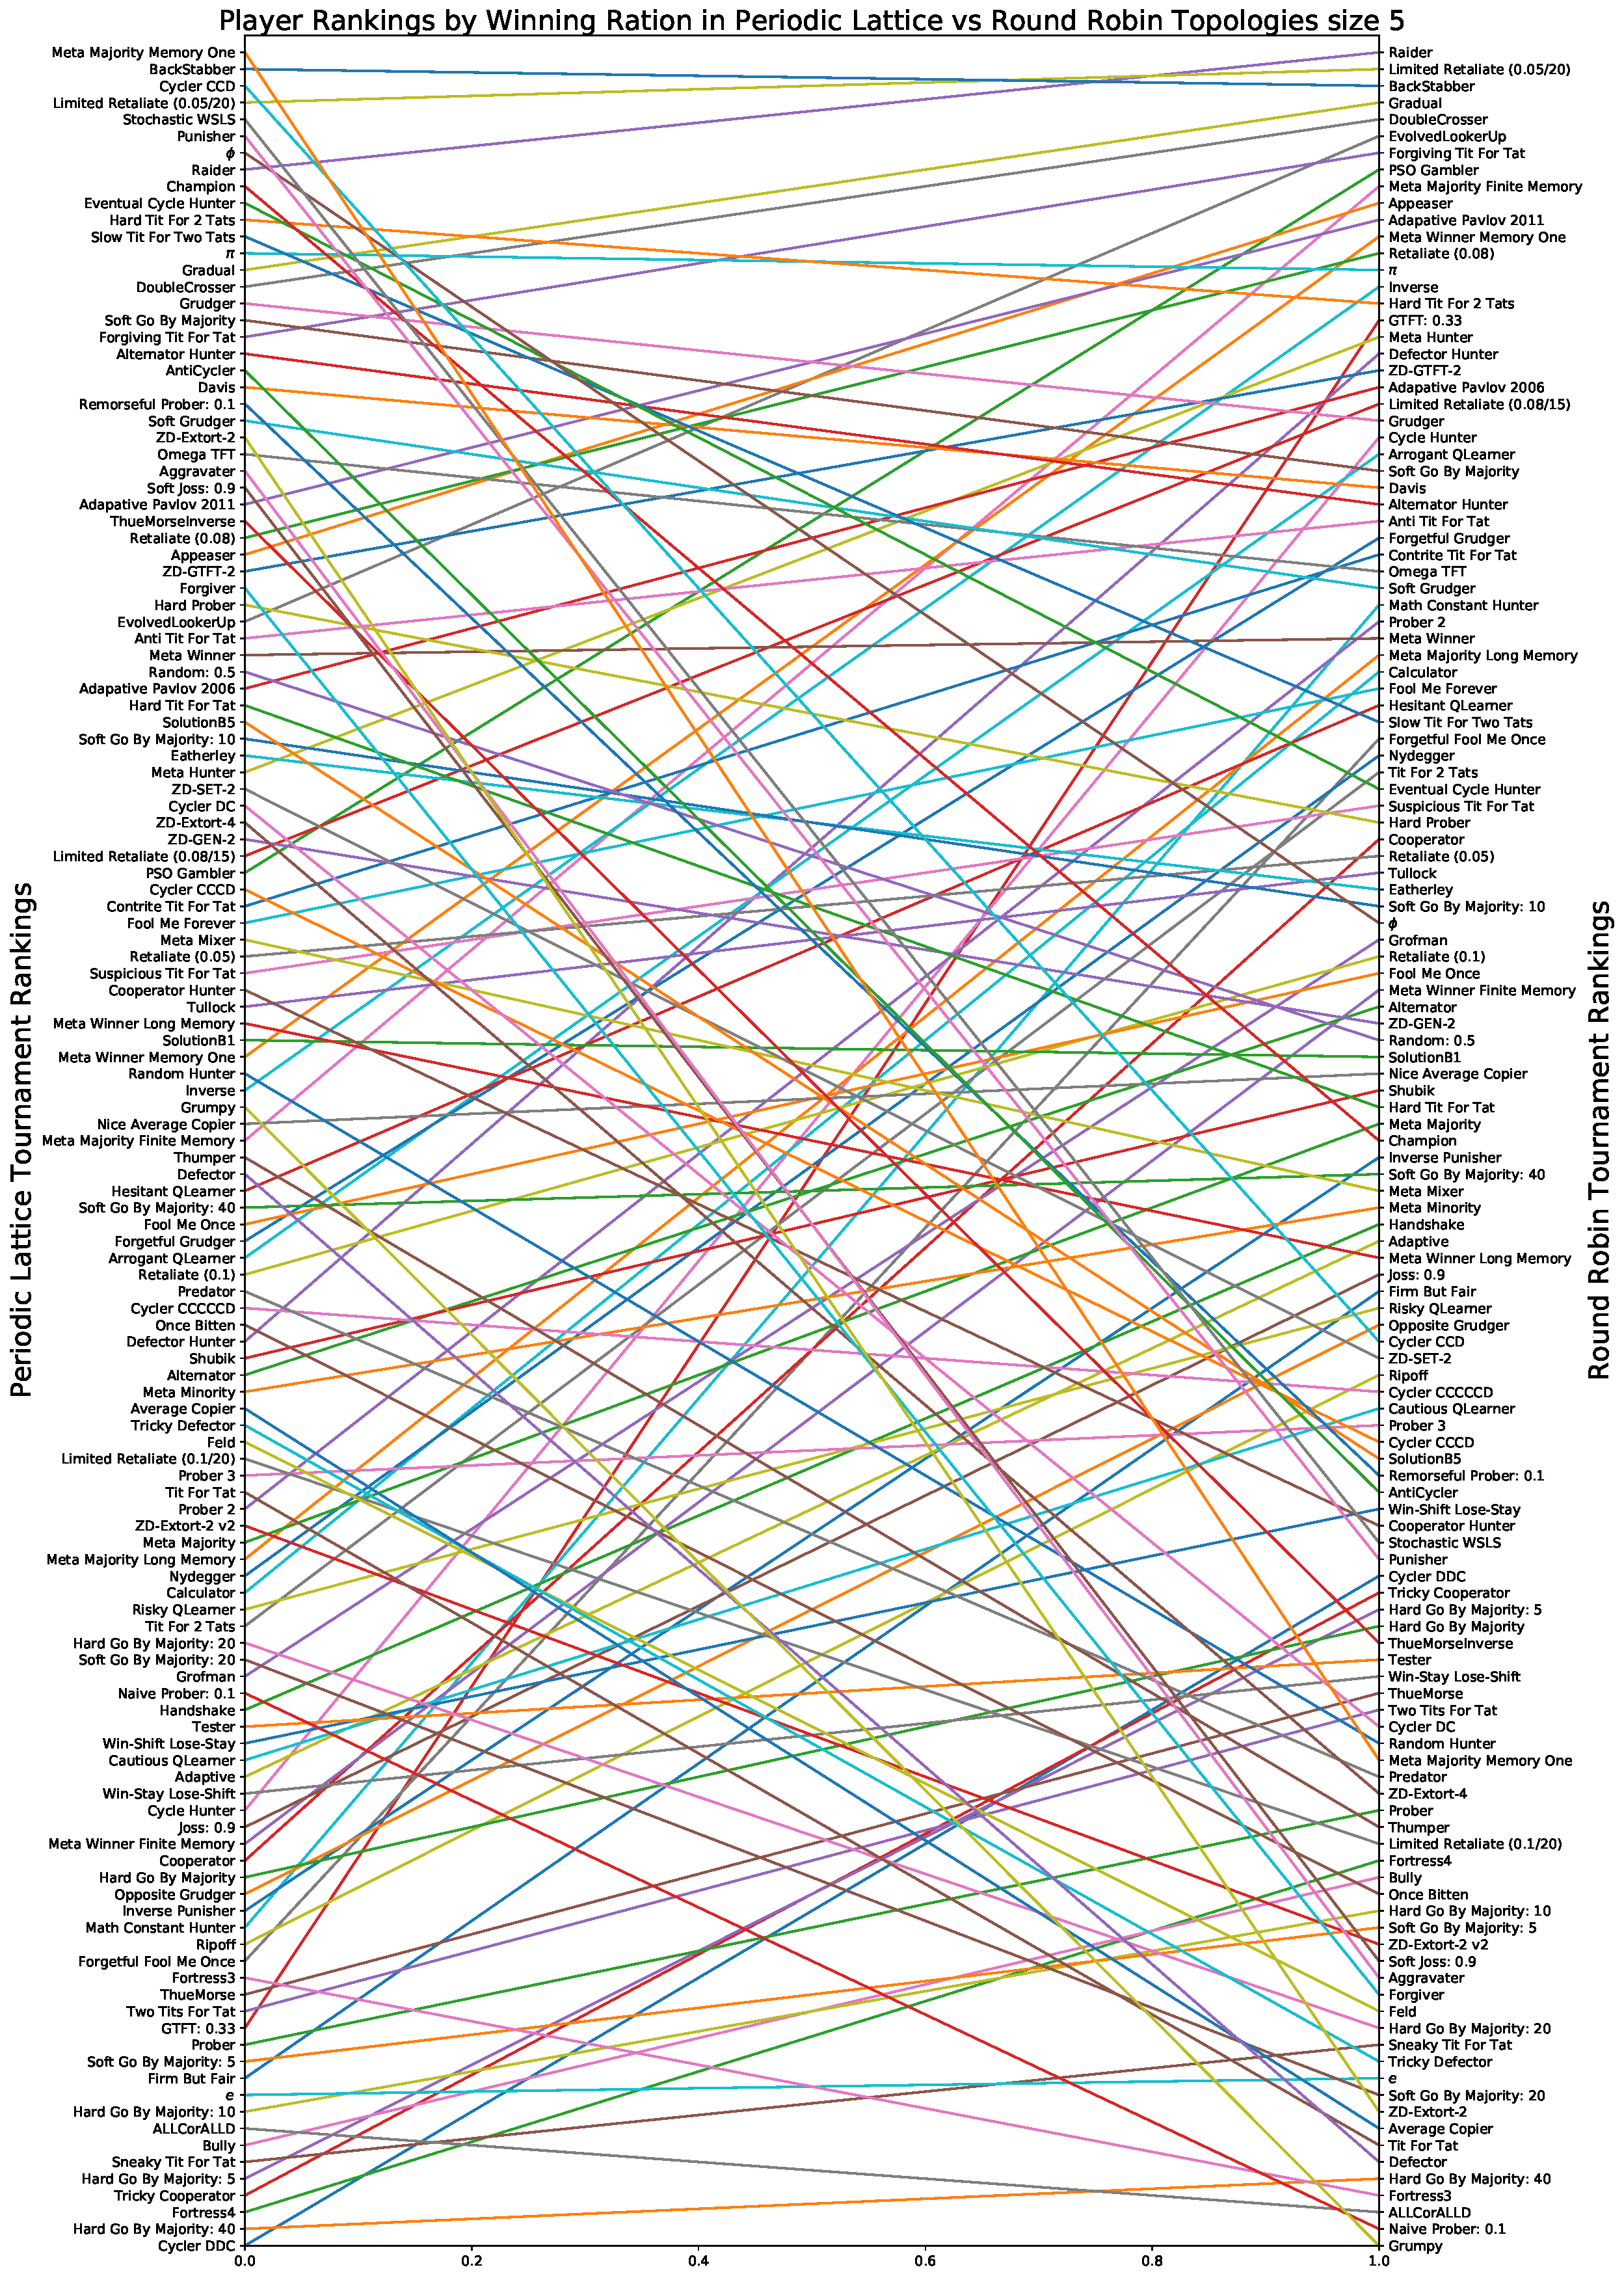
\includegraphics[width=\linewidth]{chapter-three/lines-lattice-round-robin-5.pdf}\
	\caption{Periodic Lattice vs Round
	Robin topologies size 5}
	\label{fig:winning-rankings-five-l-r}
\end{figure}

\begin{figure}[H]
	\centering
	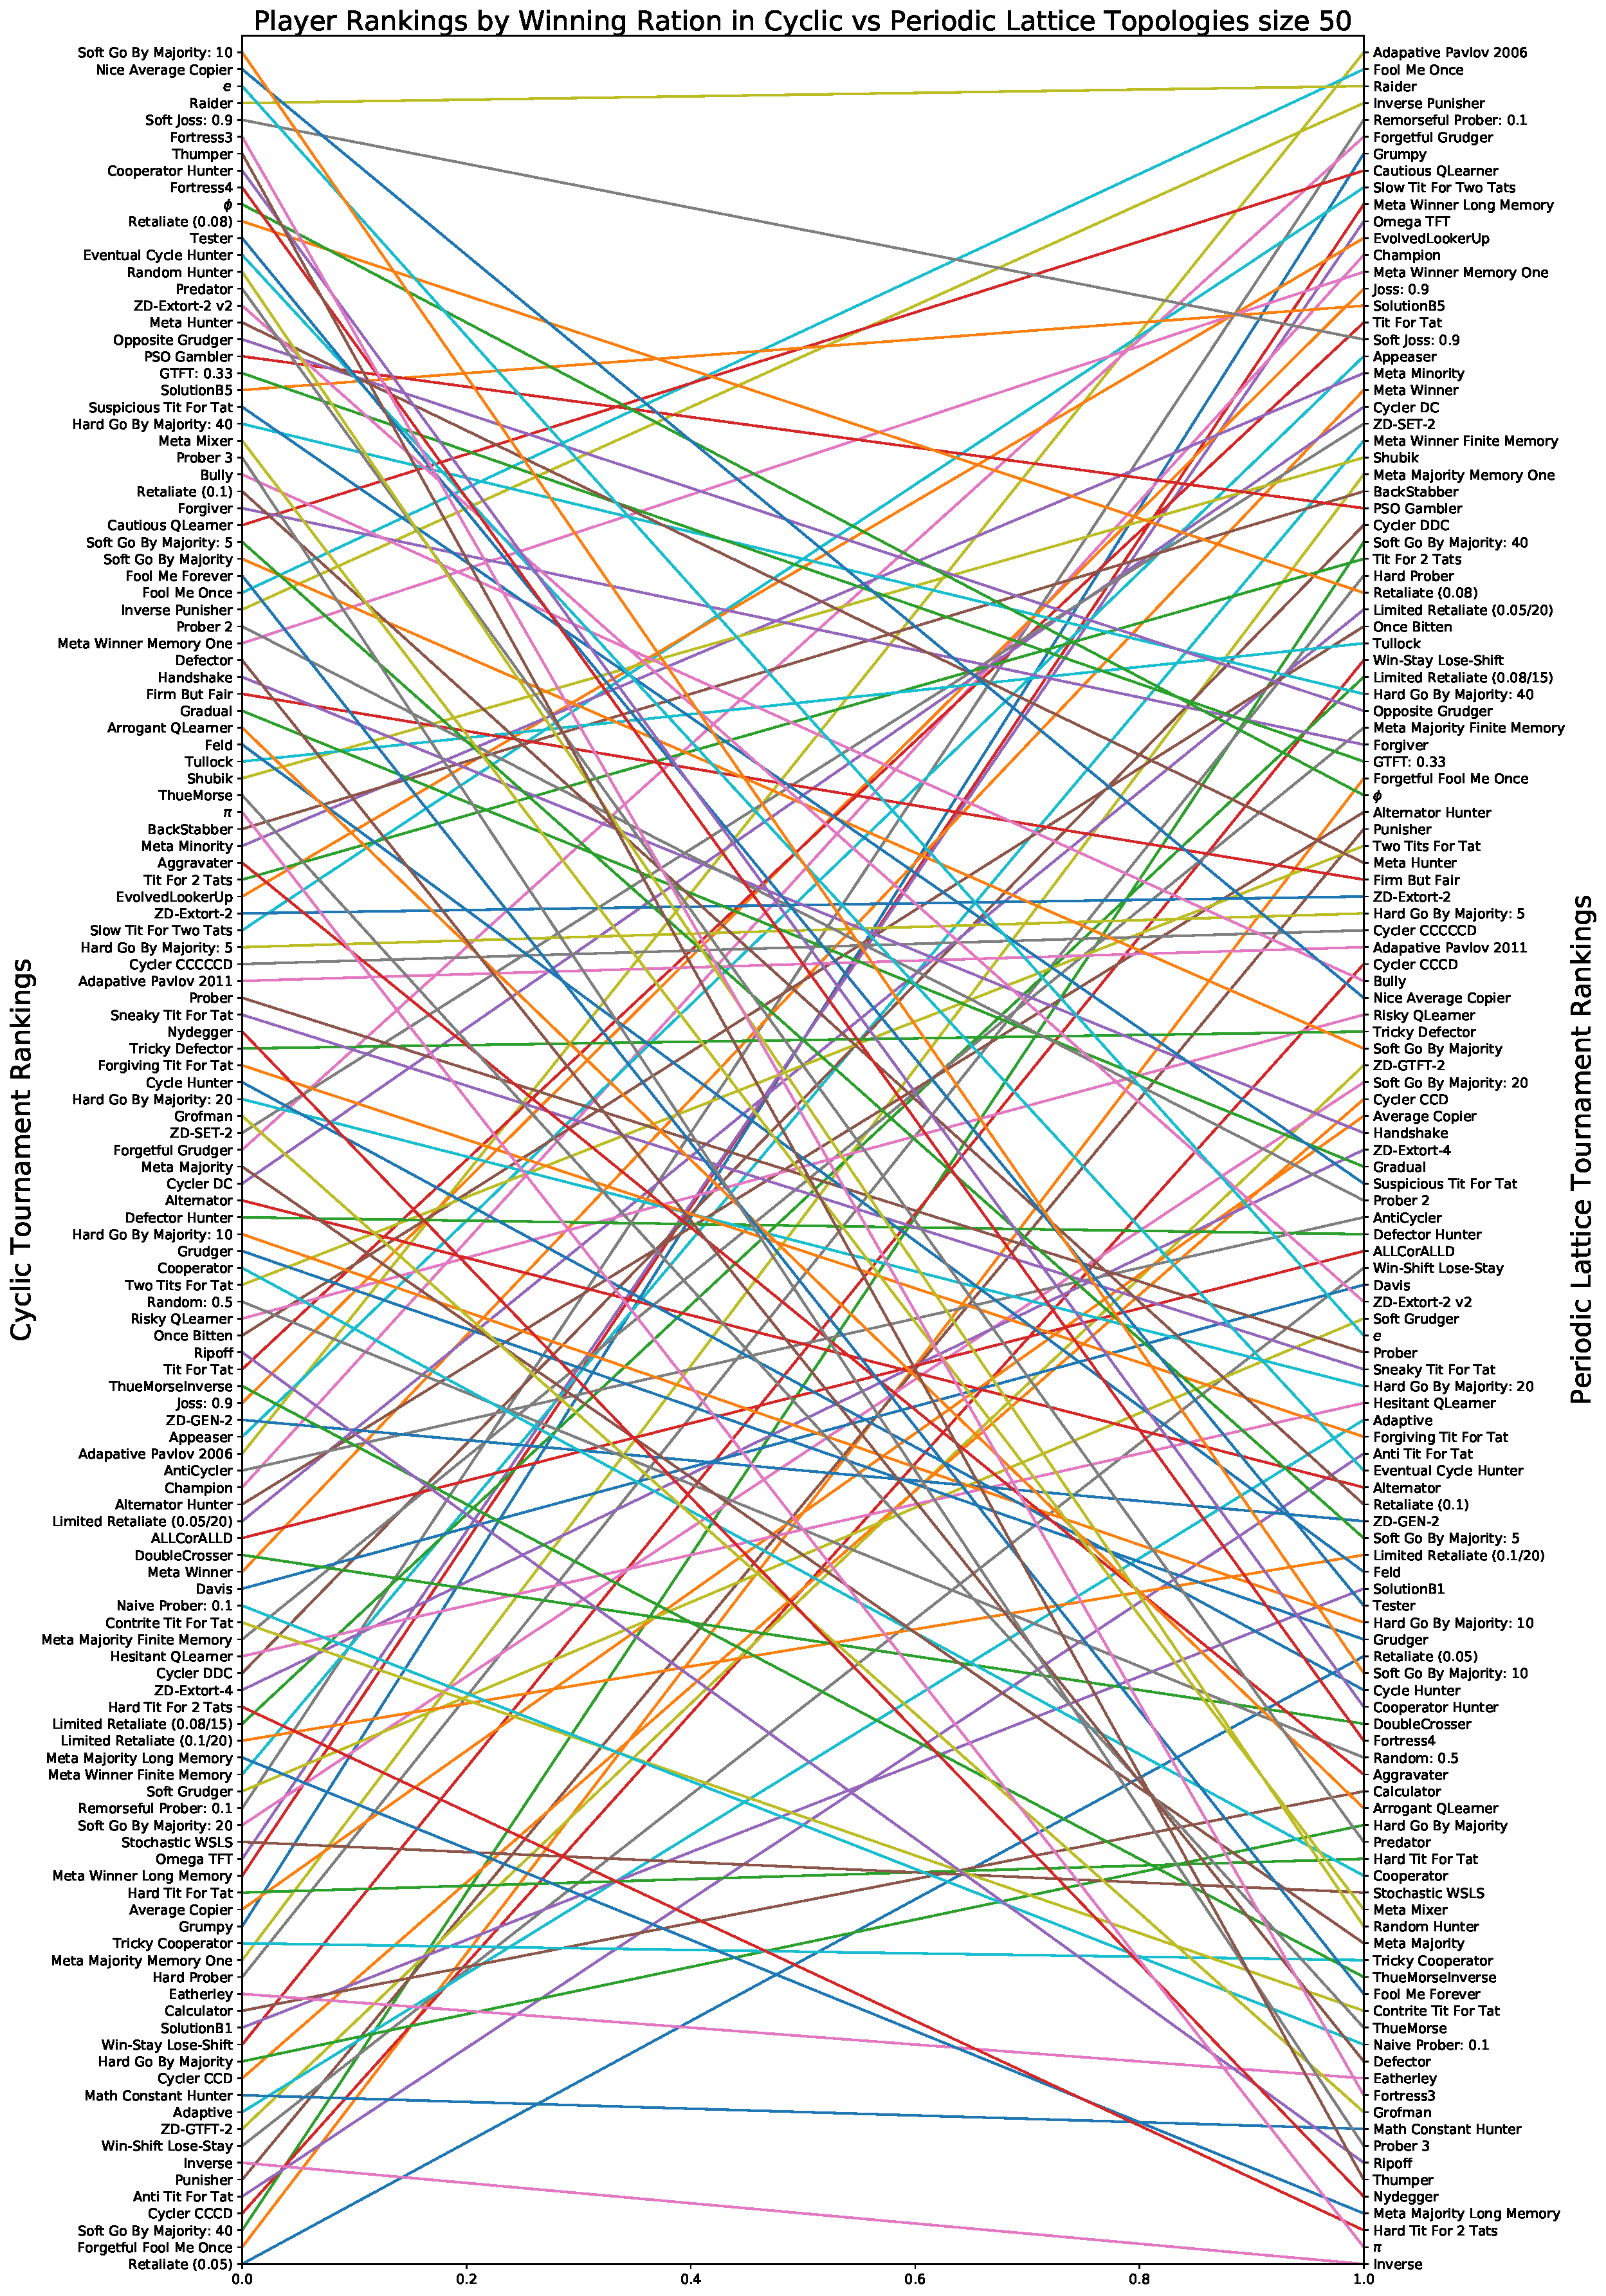
\includegraphics[width=\linewidth]{chapter-three/lines-cyclic-lattice-50.pdf}
	\caption{Cyclic vs Periodic Lattice topologies size 50}
	\label{fig:winning-rankings-fifty-c-l}
\end{figure}

\begin{figure}[H]
	\centering
	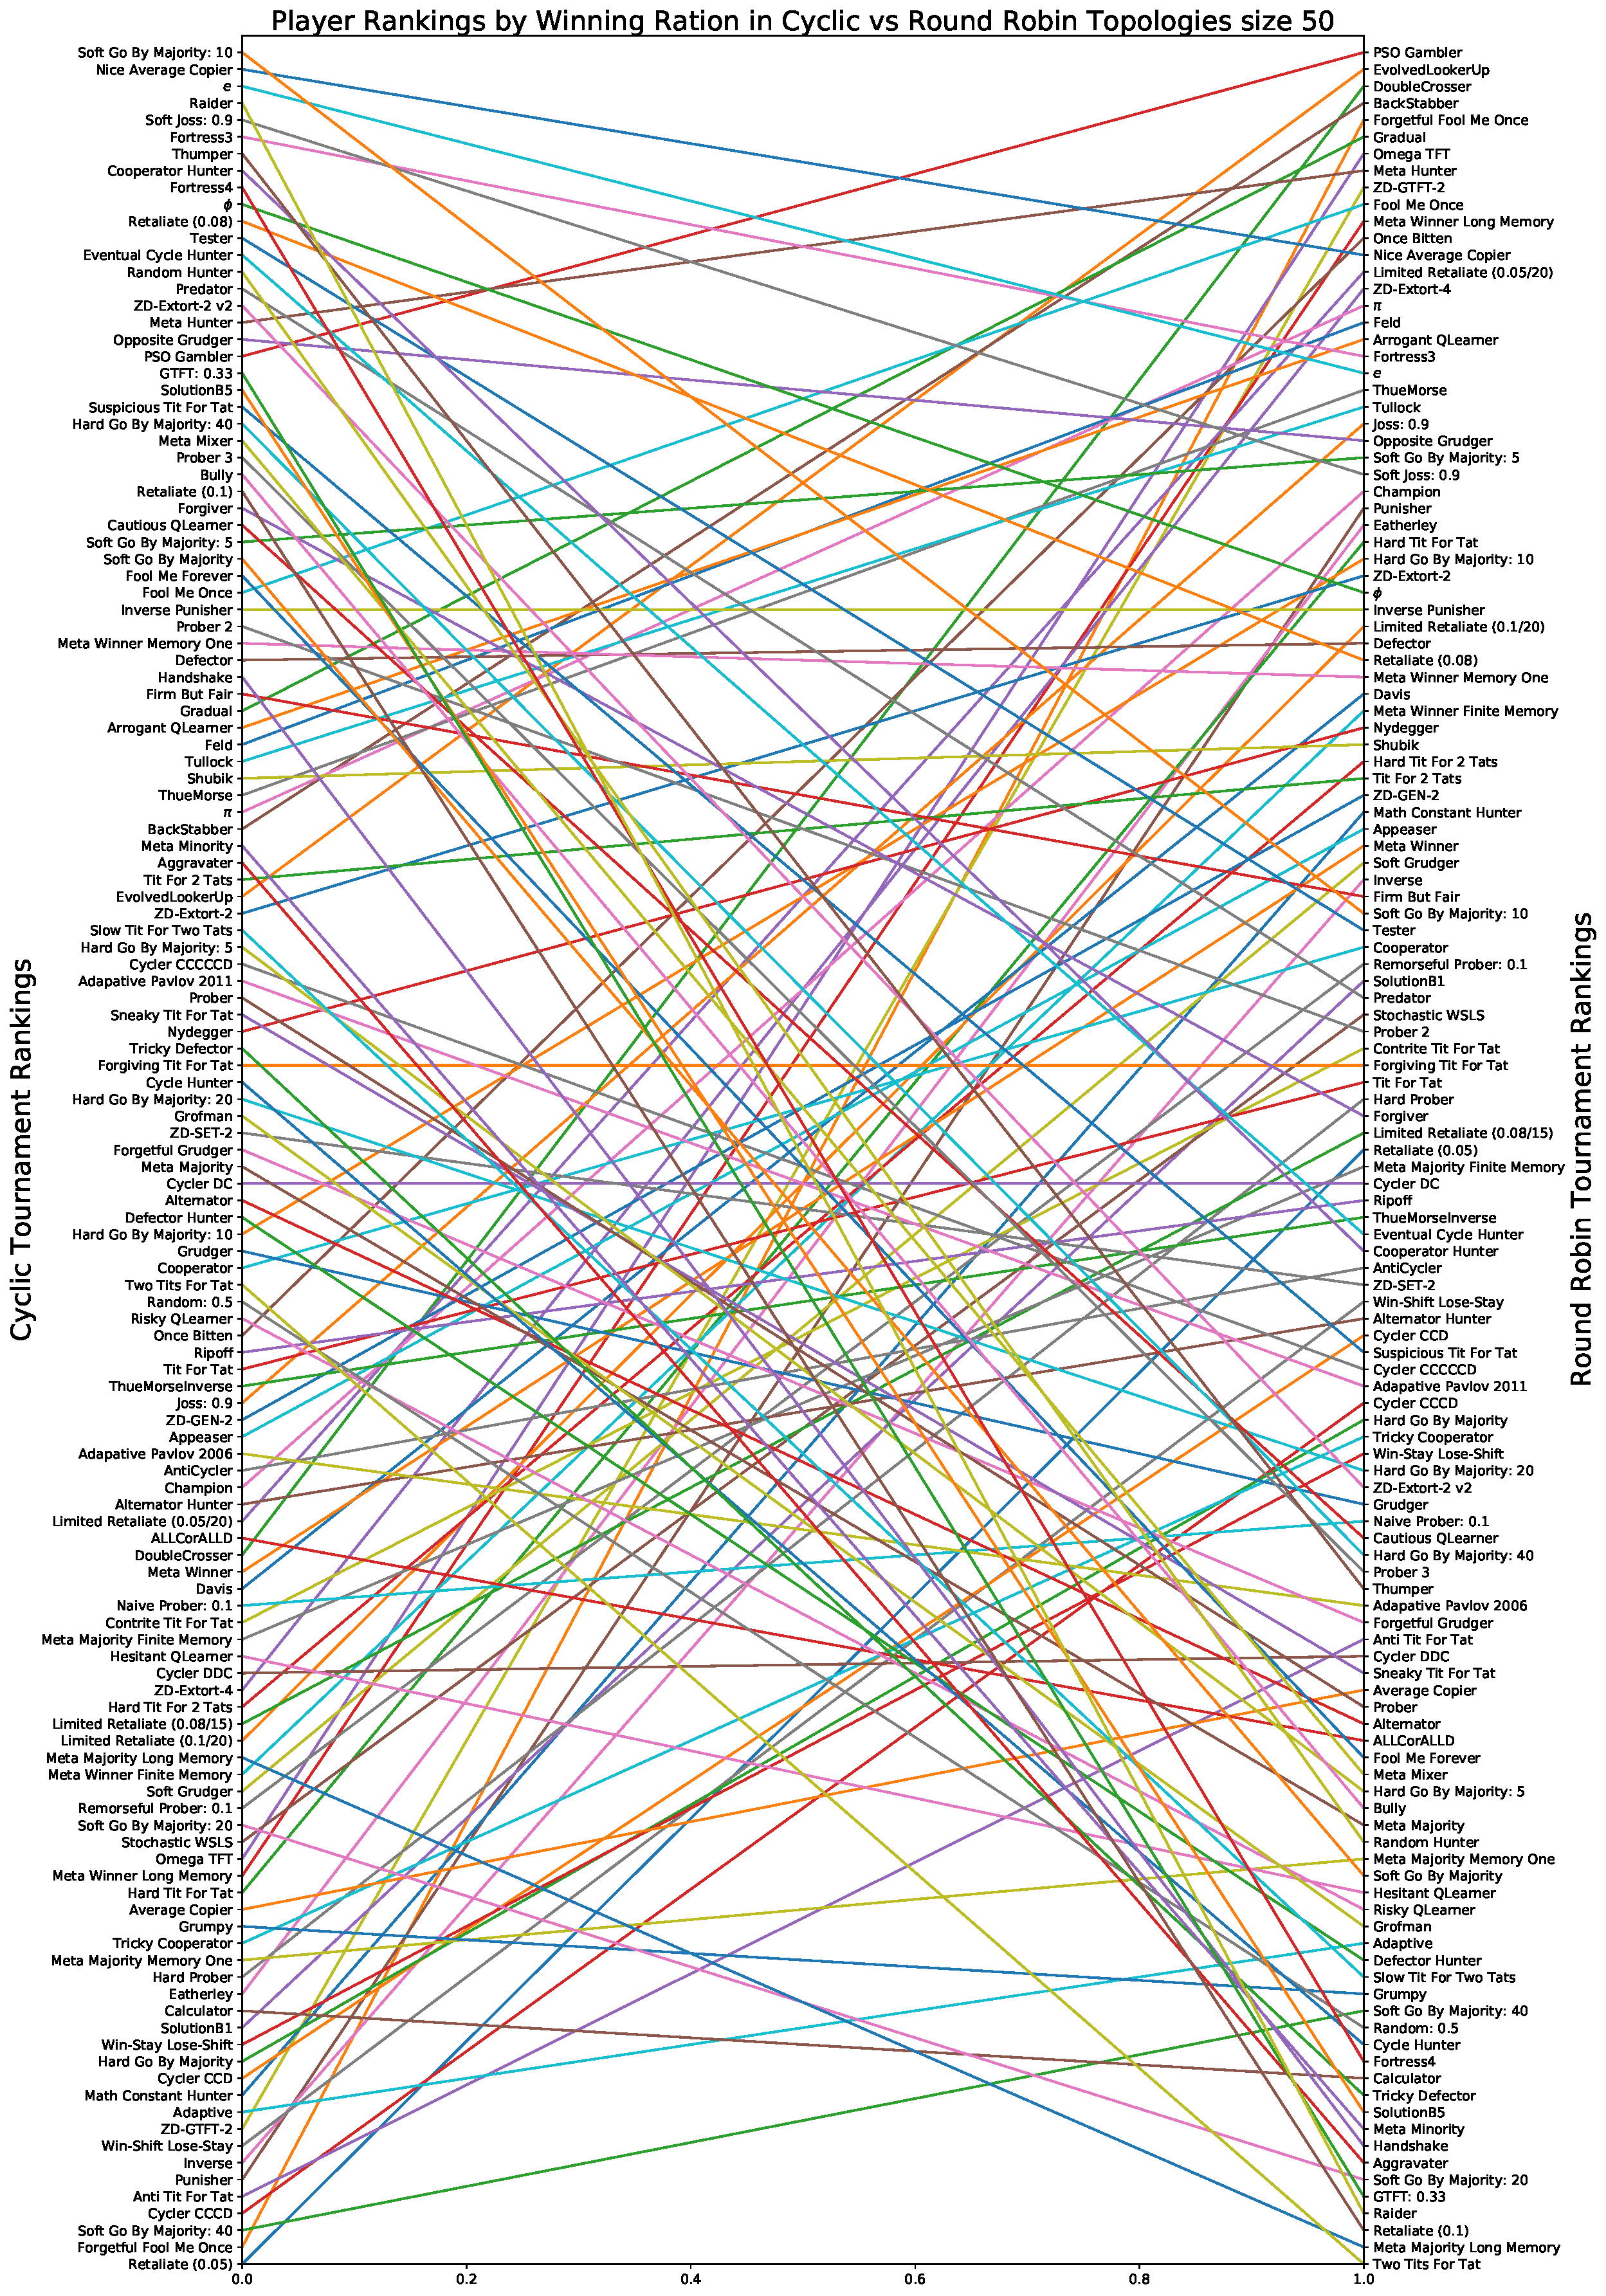
\includegraphics[width=\linewidth]{chapter-three/lines-cyclic-round-robin-50.pdf}
	\caption{Cyclic vs Round Robin topologies size 50}
	\label{fig:winning-rankings-fifty-c-r}
\end{figure}

\begin{figure}[H]
	\centering
	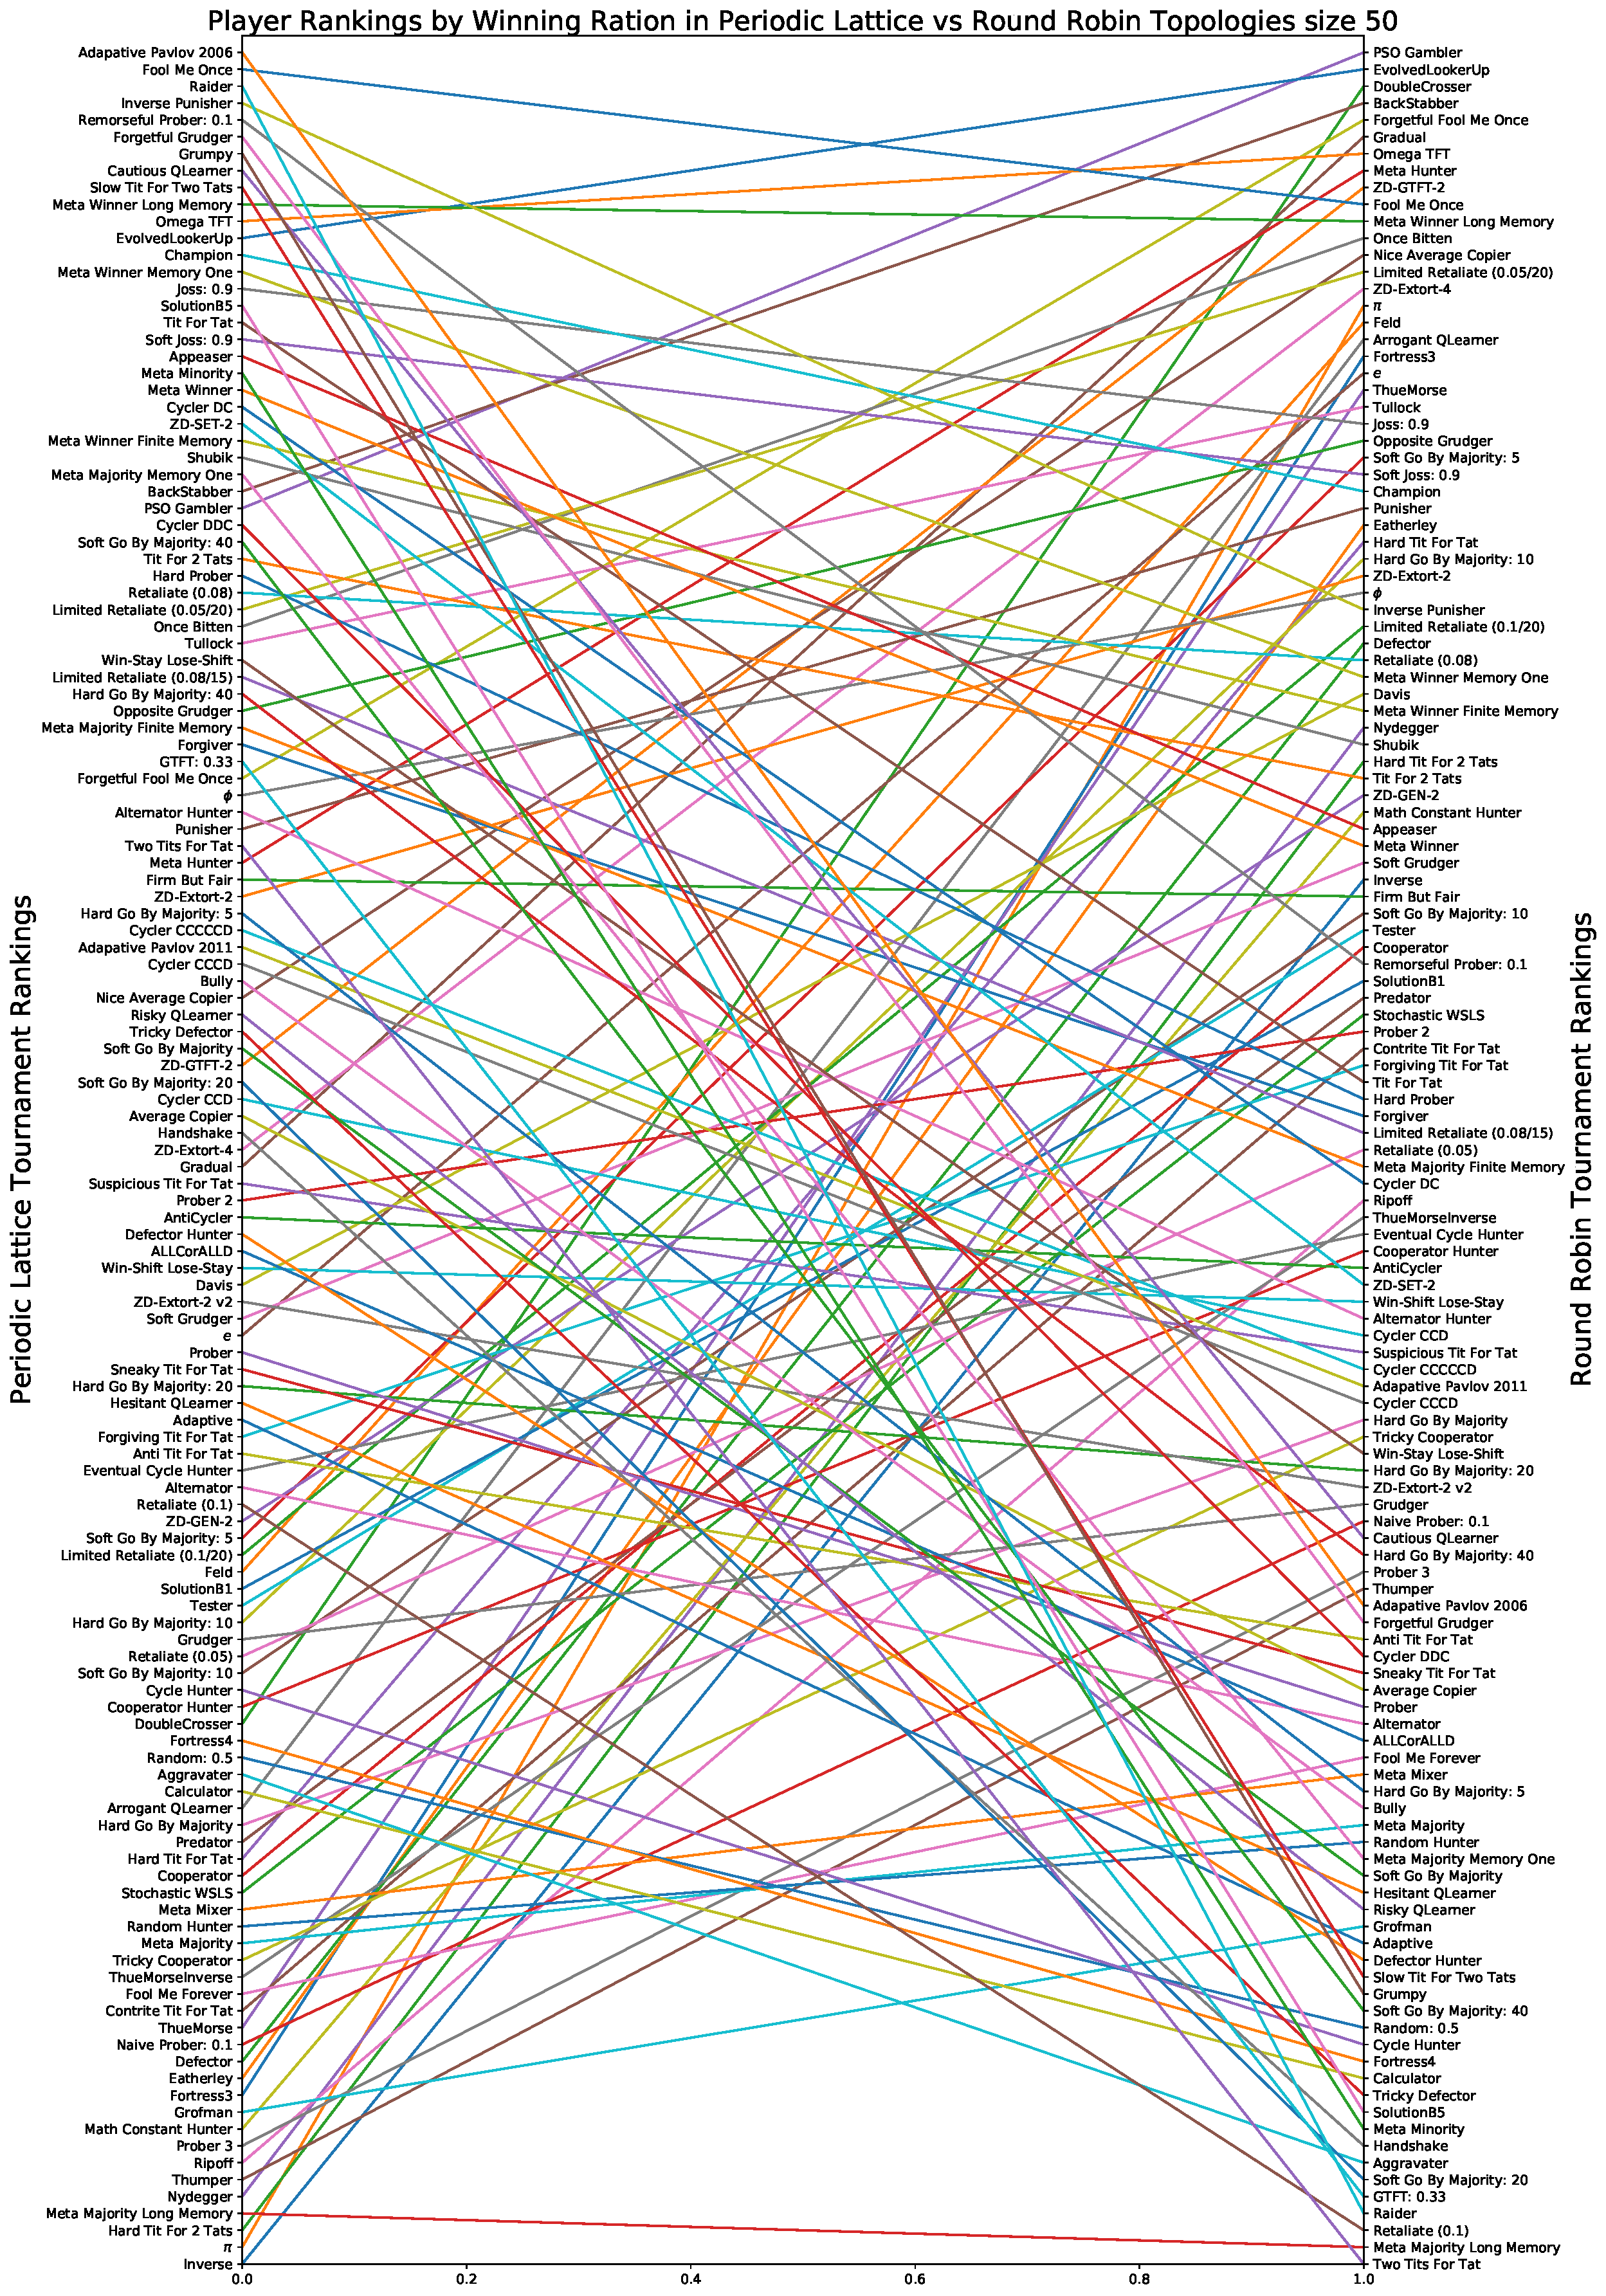
\includegraphics[width=\linewidth]{chapter-three/lines-lattice-round-robin-50.pdf}
	\caption{Periodic Lattice vs Round Robin topologies size 50}
	\label{fig:winning-rankings-fifty-l-r}
\end{figure}

The strategies can be classified based on the number of tournament
participations. For tournament size 5, 9 classes have been created for
the cyclic and the periodic lattice topologies, [10, 20, 30, 40, 50, 60, 70, 80, 90].
For tournament
size 50, [270, 280, 290, 310, 320, 330, 340, 350, 360, 370, 380, 390, 400, 410,
420, 430, 440, 450, 460, 470, 570]. Round robin topology
experiments were classified as [1, 2, 3, 4, 5, 6, 7, 8, 9] and
[27, 28, 29, 31, 32, 33, 34, 35, 36, 37, 38, 39, 40, 41, 42, 43, 44, 45, 46, 47, 57],
respectively. The winning ratios were plotted against participation number
in Figure~\ref{fig:winning-ratio-participations-five} and Figure~\ref{fig:winning-ratio-participations-fifty}.
An ANOVA analysis was used to analyze the importance of the
differences in the winning ratios among the participating groups.

Primarily, the normality of the ration has been tested. For all 6 experiments,
the winning ratio, is not normally distributed. As all \(p\) values are
less that 0.05. Thus, a non parametric test has been used instead. The equivelent
non parametric ANOVA test is the Kruskal Wallis test. The Python library
\texttt{scipy}, provided the functions necessary for the tests.

The results, for a tournament of size equal to 5, the difference
of ratios between the participations groups is significant (\(p\) values
are lower that 0.05). Shown in Figure~\ref{fig:winning-ratio-participations-five},
are violin plots of the winning ratio against number of participations.
A positive trend can be spotted for the lattice and a negative for the cyclic
and round robin topologies.

Equivalently, in Figure~\ref{fig:winning-ratio-participations-fifty}, violin plots for
tournament size 50 are displayed. For all three topologies, there is there  a s
statistically significant difference. The specific groups that different are not
clear. Post-hoc analysis could be performed but will not be considered here.
Lattice topology, once again, has an positive effect, where cyclic a negative.

\begin{figure}[H]
	\centering

	\begin{subfigure}[t]{0.75\textwidth}
		\centering
		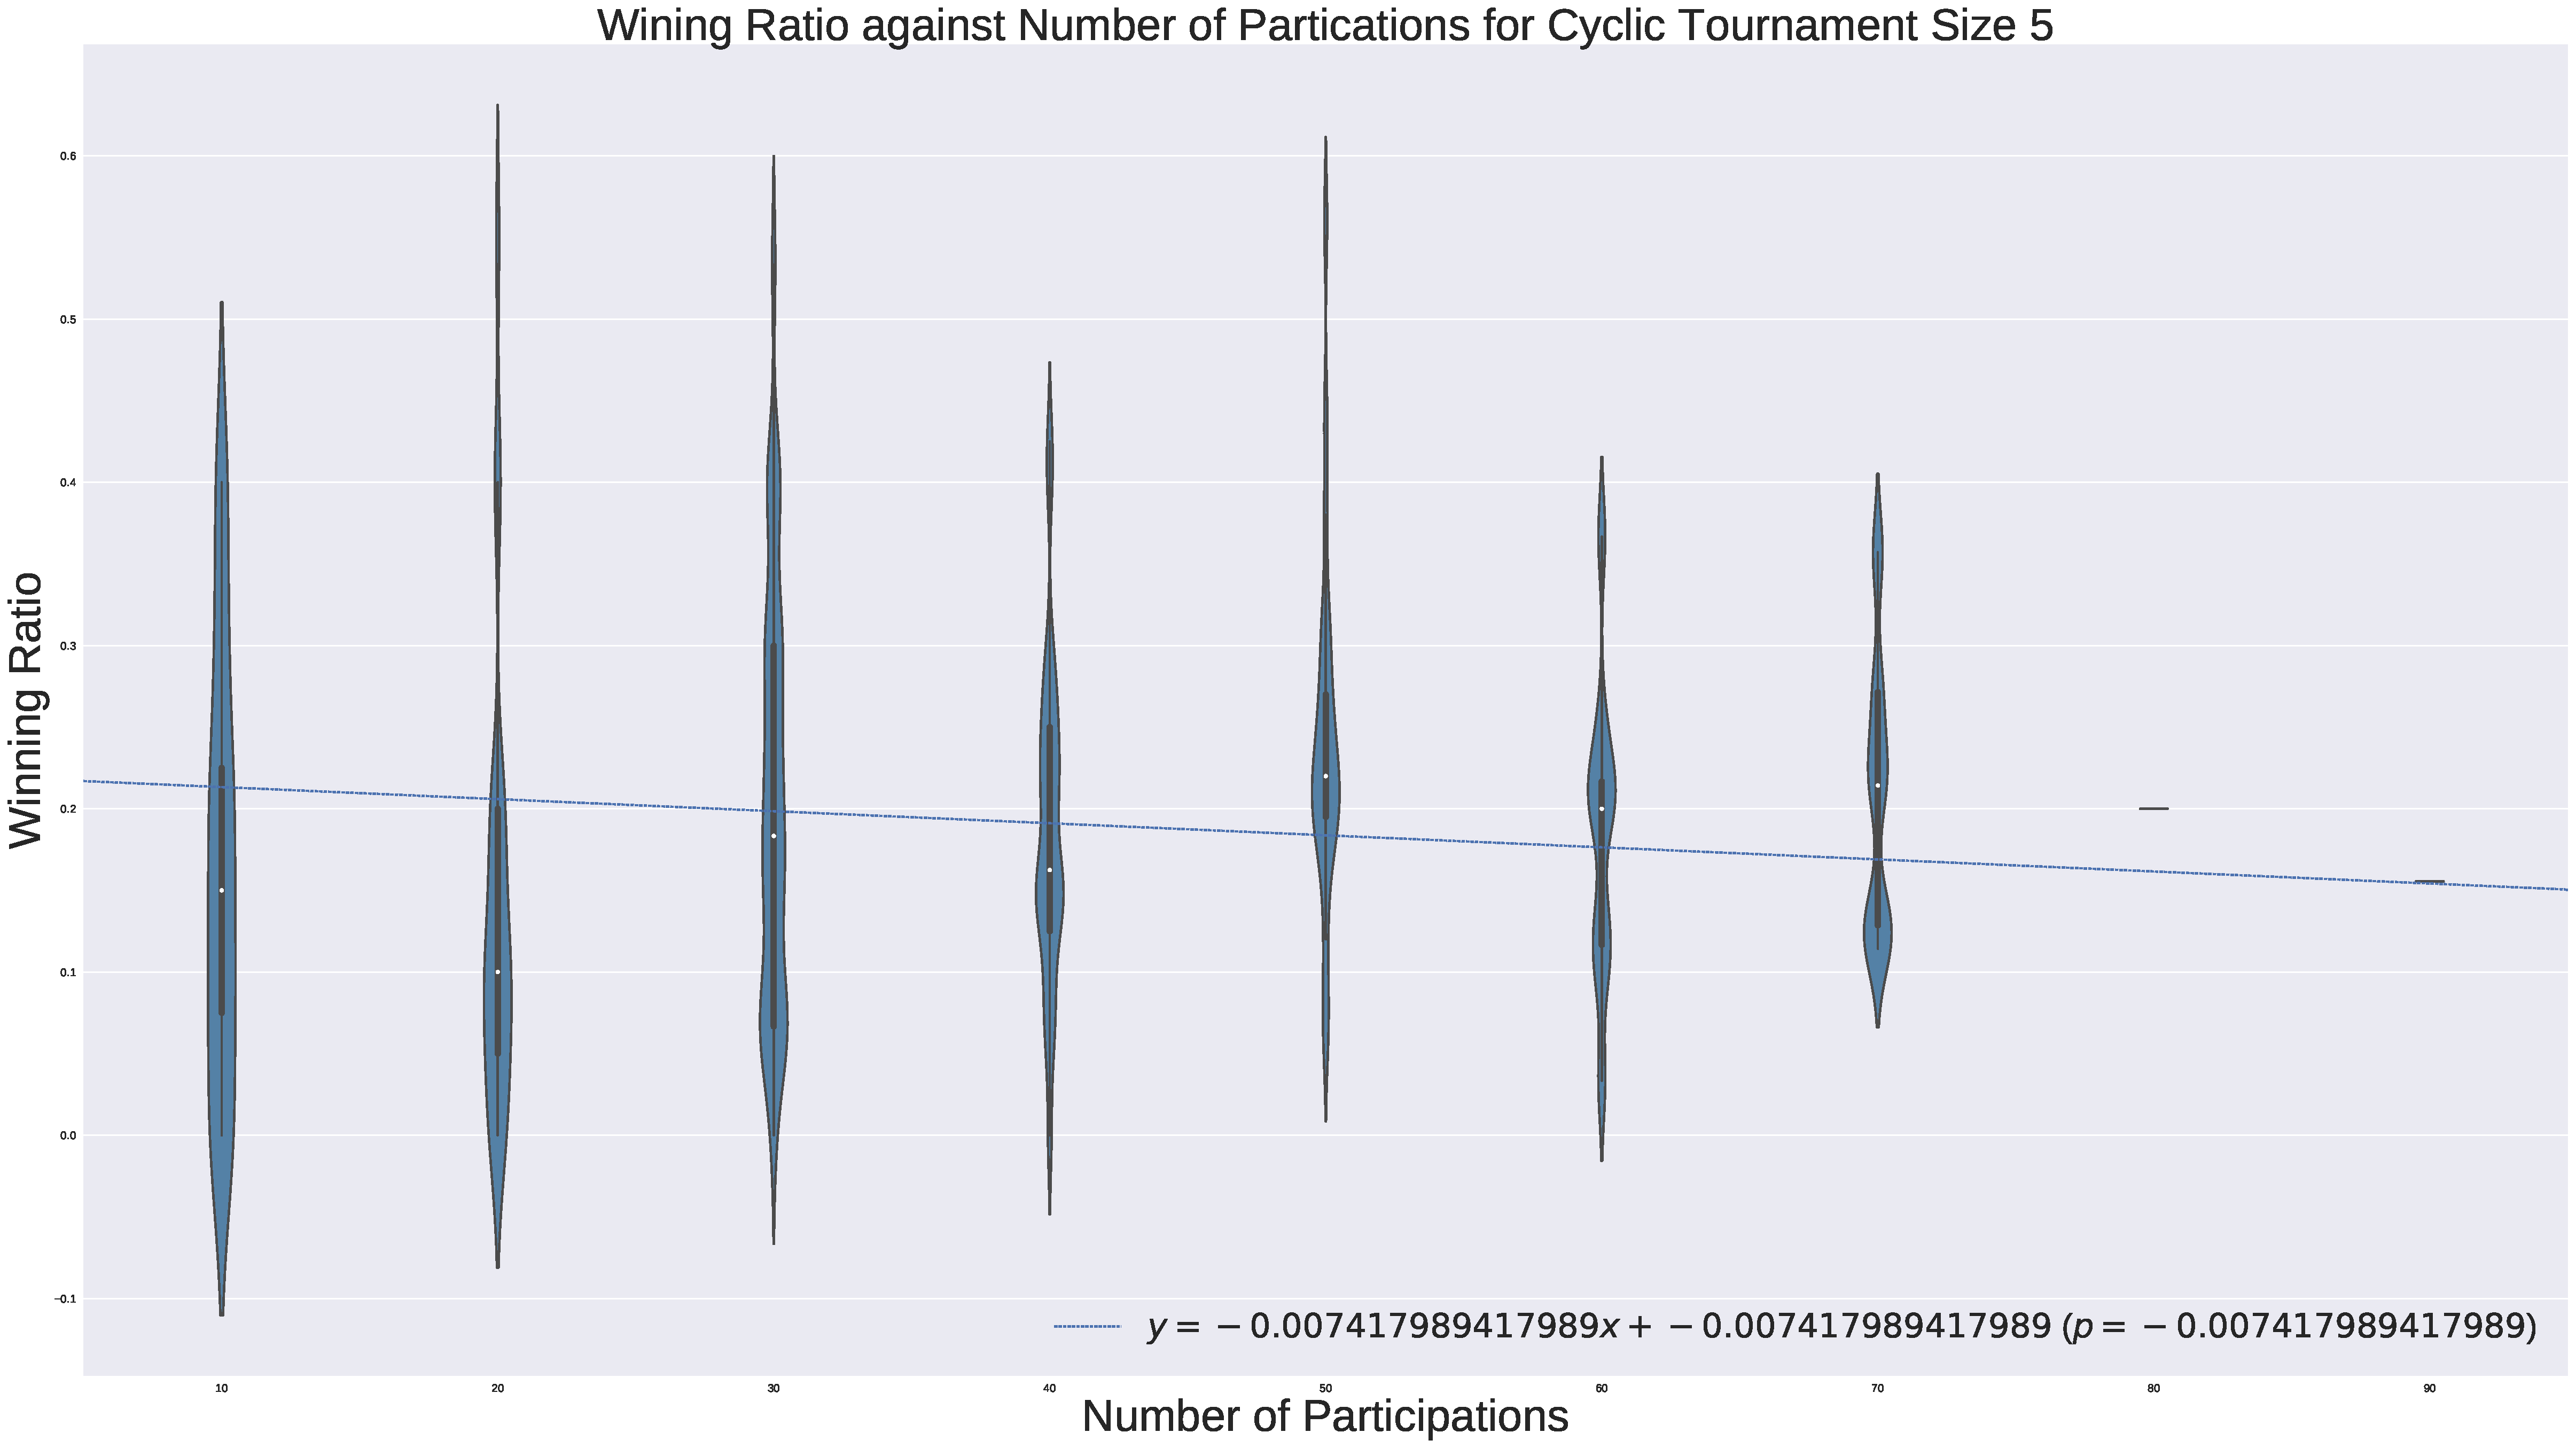
\includegraphics[width=\linewidth]{chapter-three/anova-Cyclic-5.pdf}
		\caption{Winning ratio vs number of participations cyclic tournament size 5}
	\end{subfigure}
	\hfill
	\begin{subfigure}[t]{0.75\textwidth}\centering
		\centering
		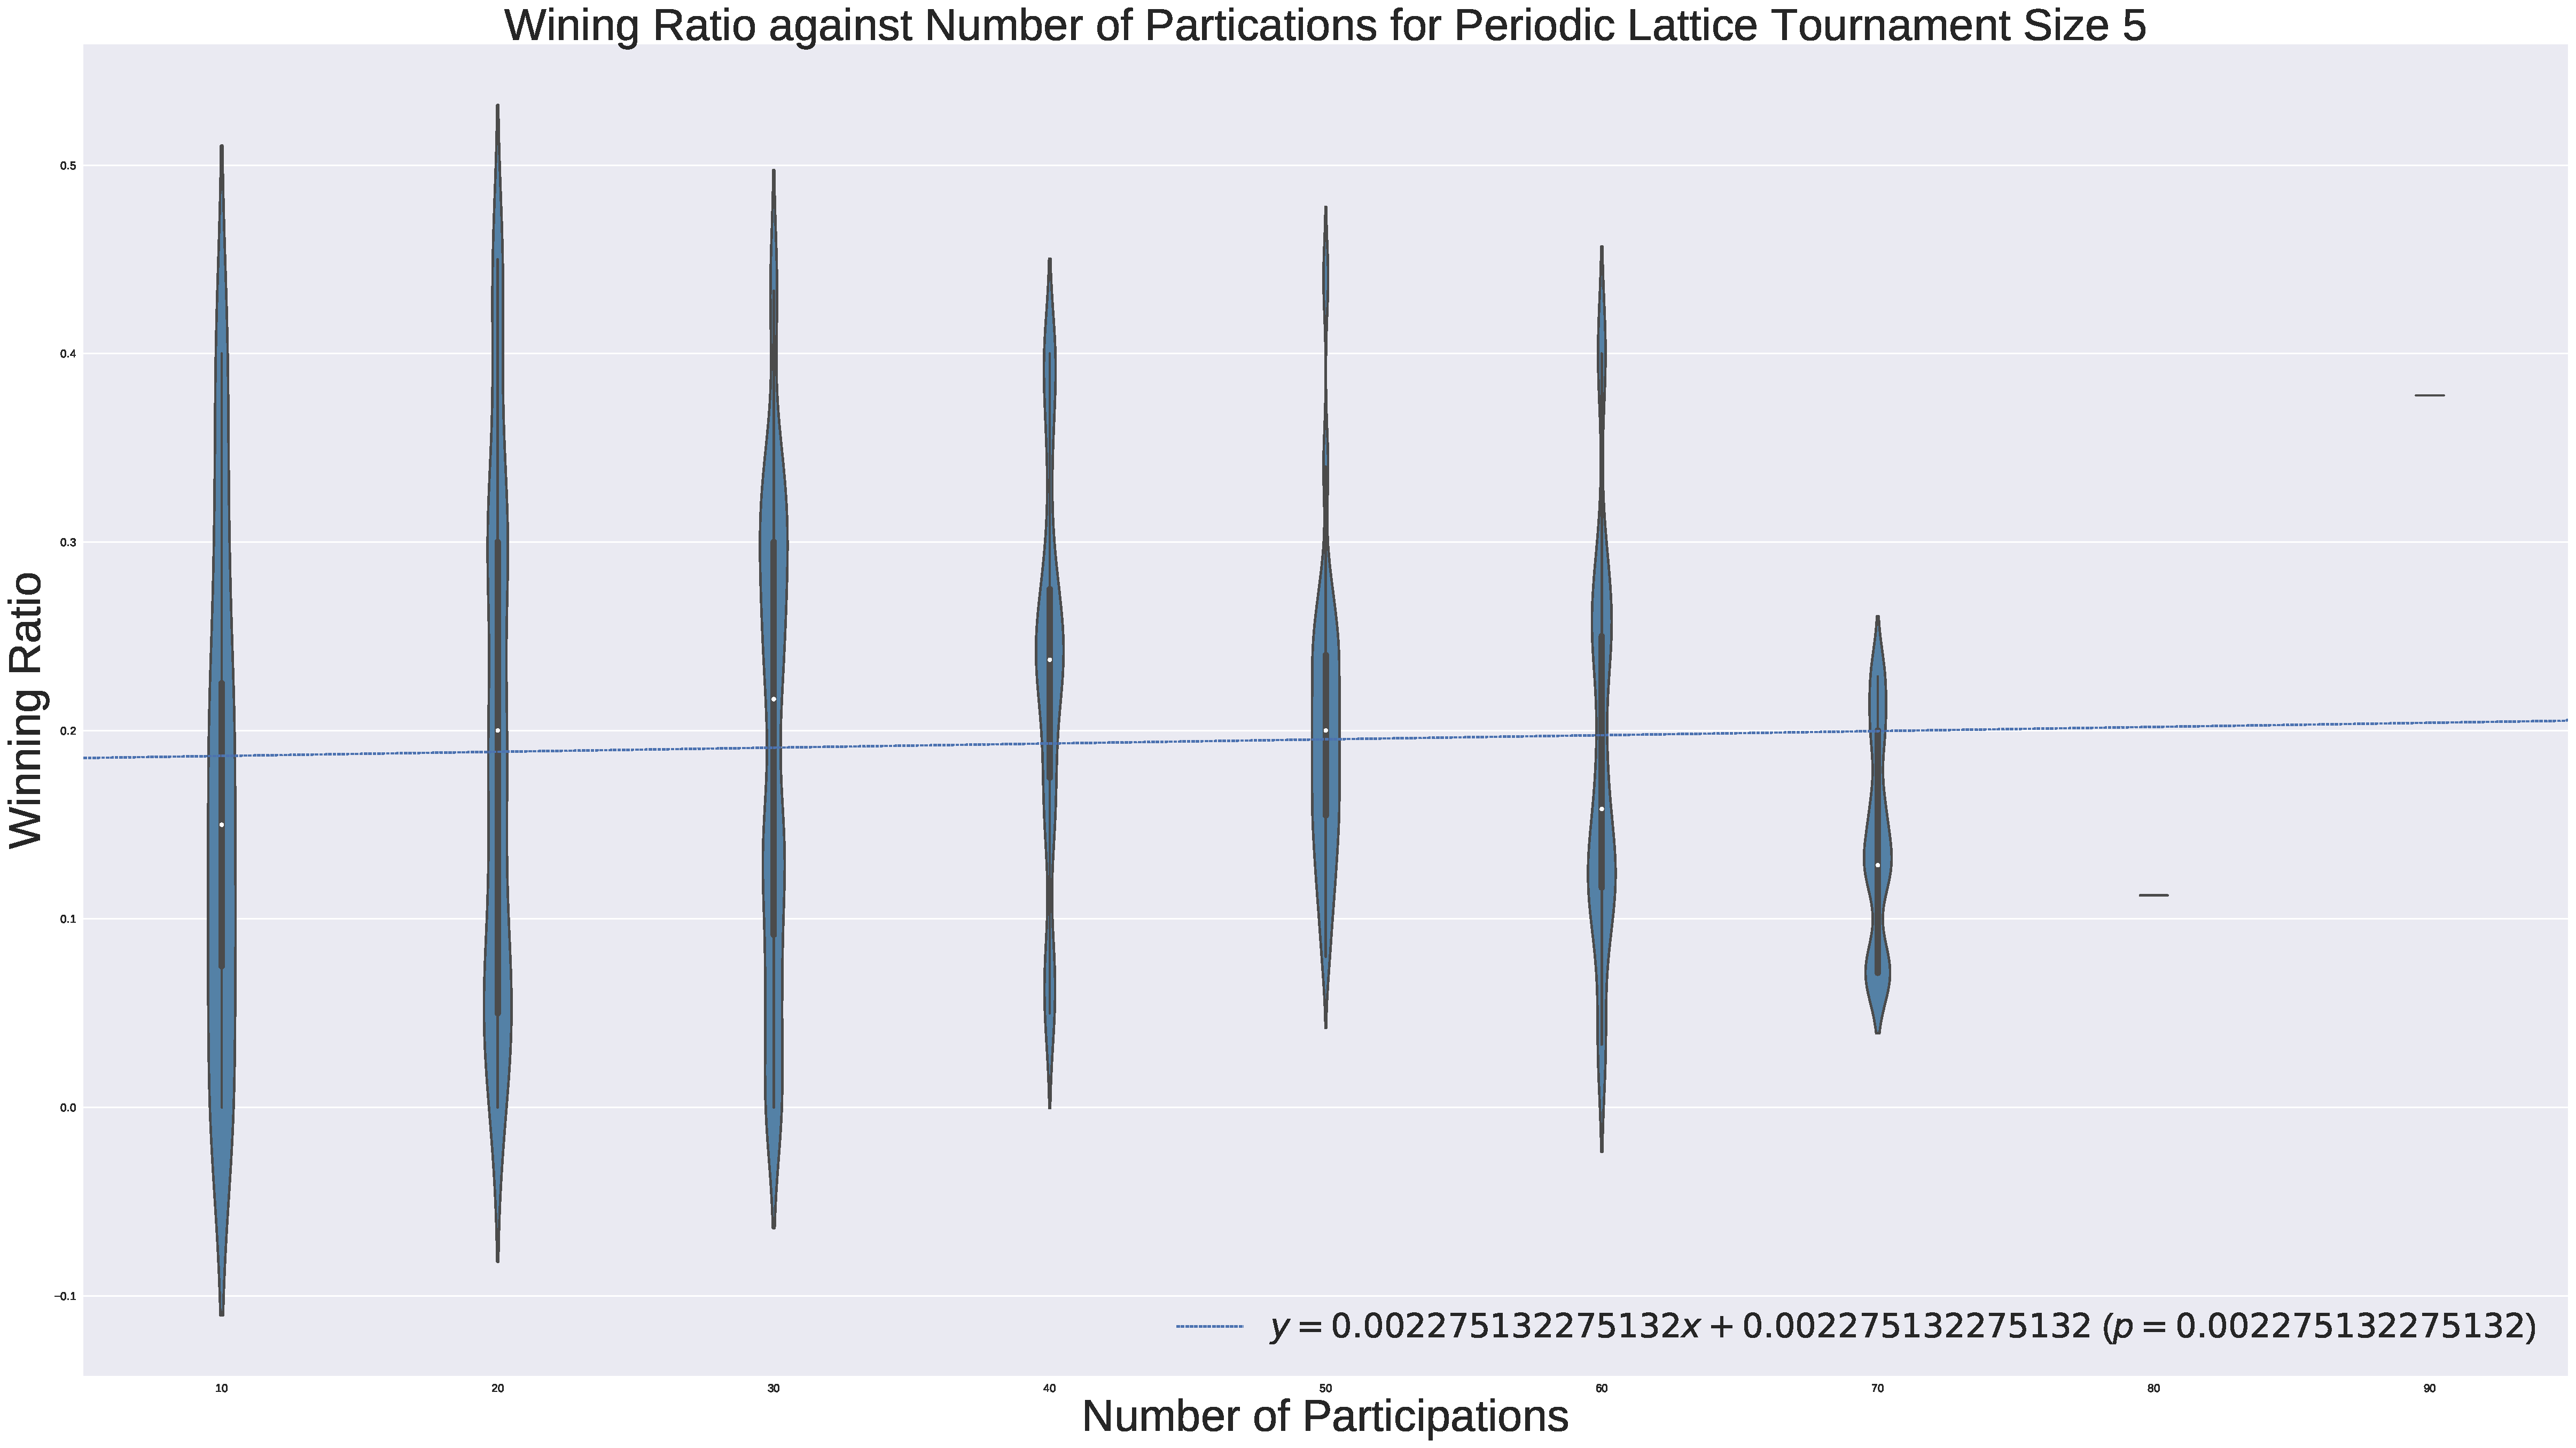
\includegraphics[width=\linewidth]{chapter-three/anova-Periodic-Lattice-5.pdf}
		\caption{Winning ratio vs number of participations periodic lattice tournament size 5}
	\end{subfigure}
	\hfill
	\begin{subfigure}[t]{0.75\textwidth}\centering
		\centering
		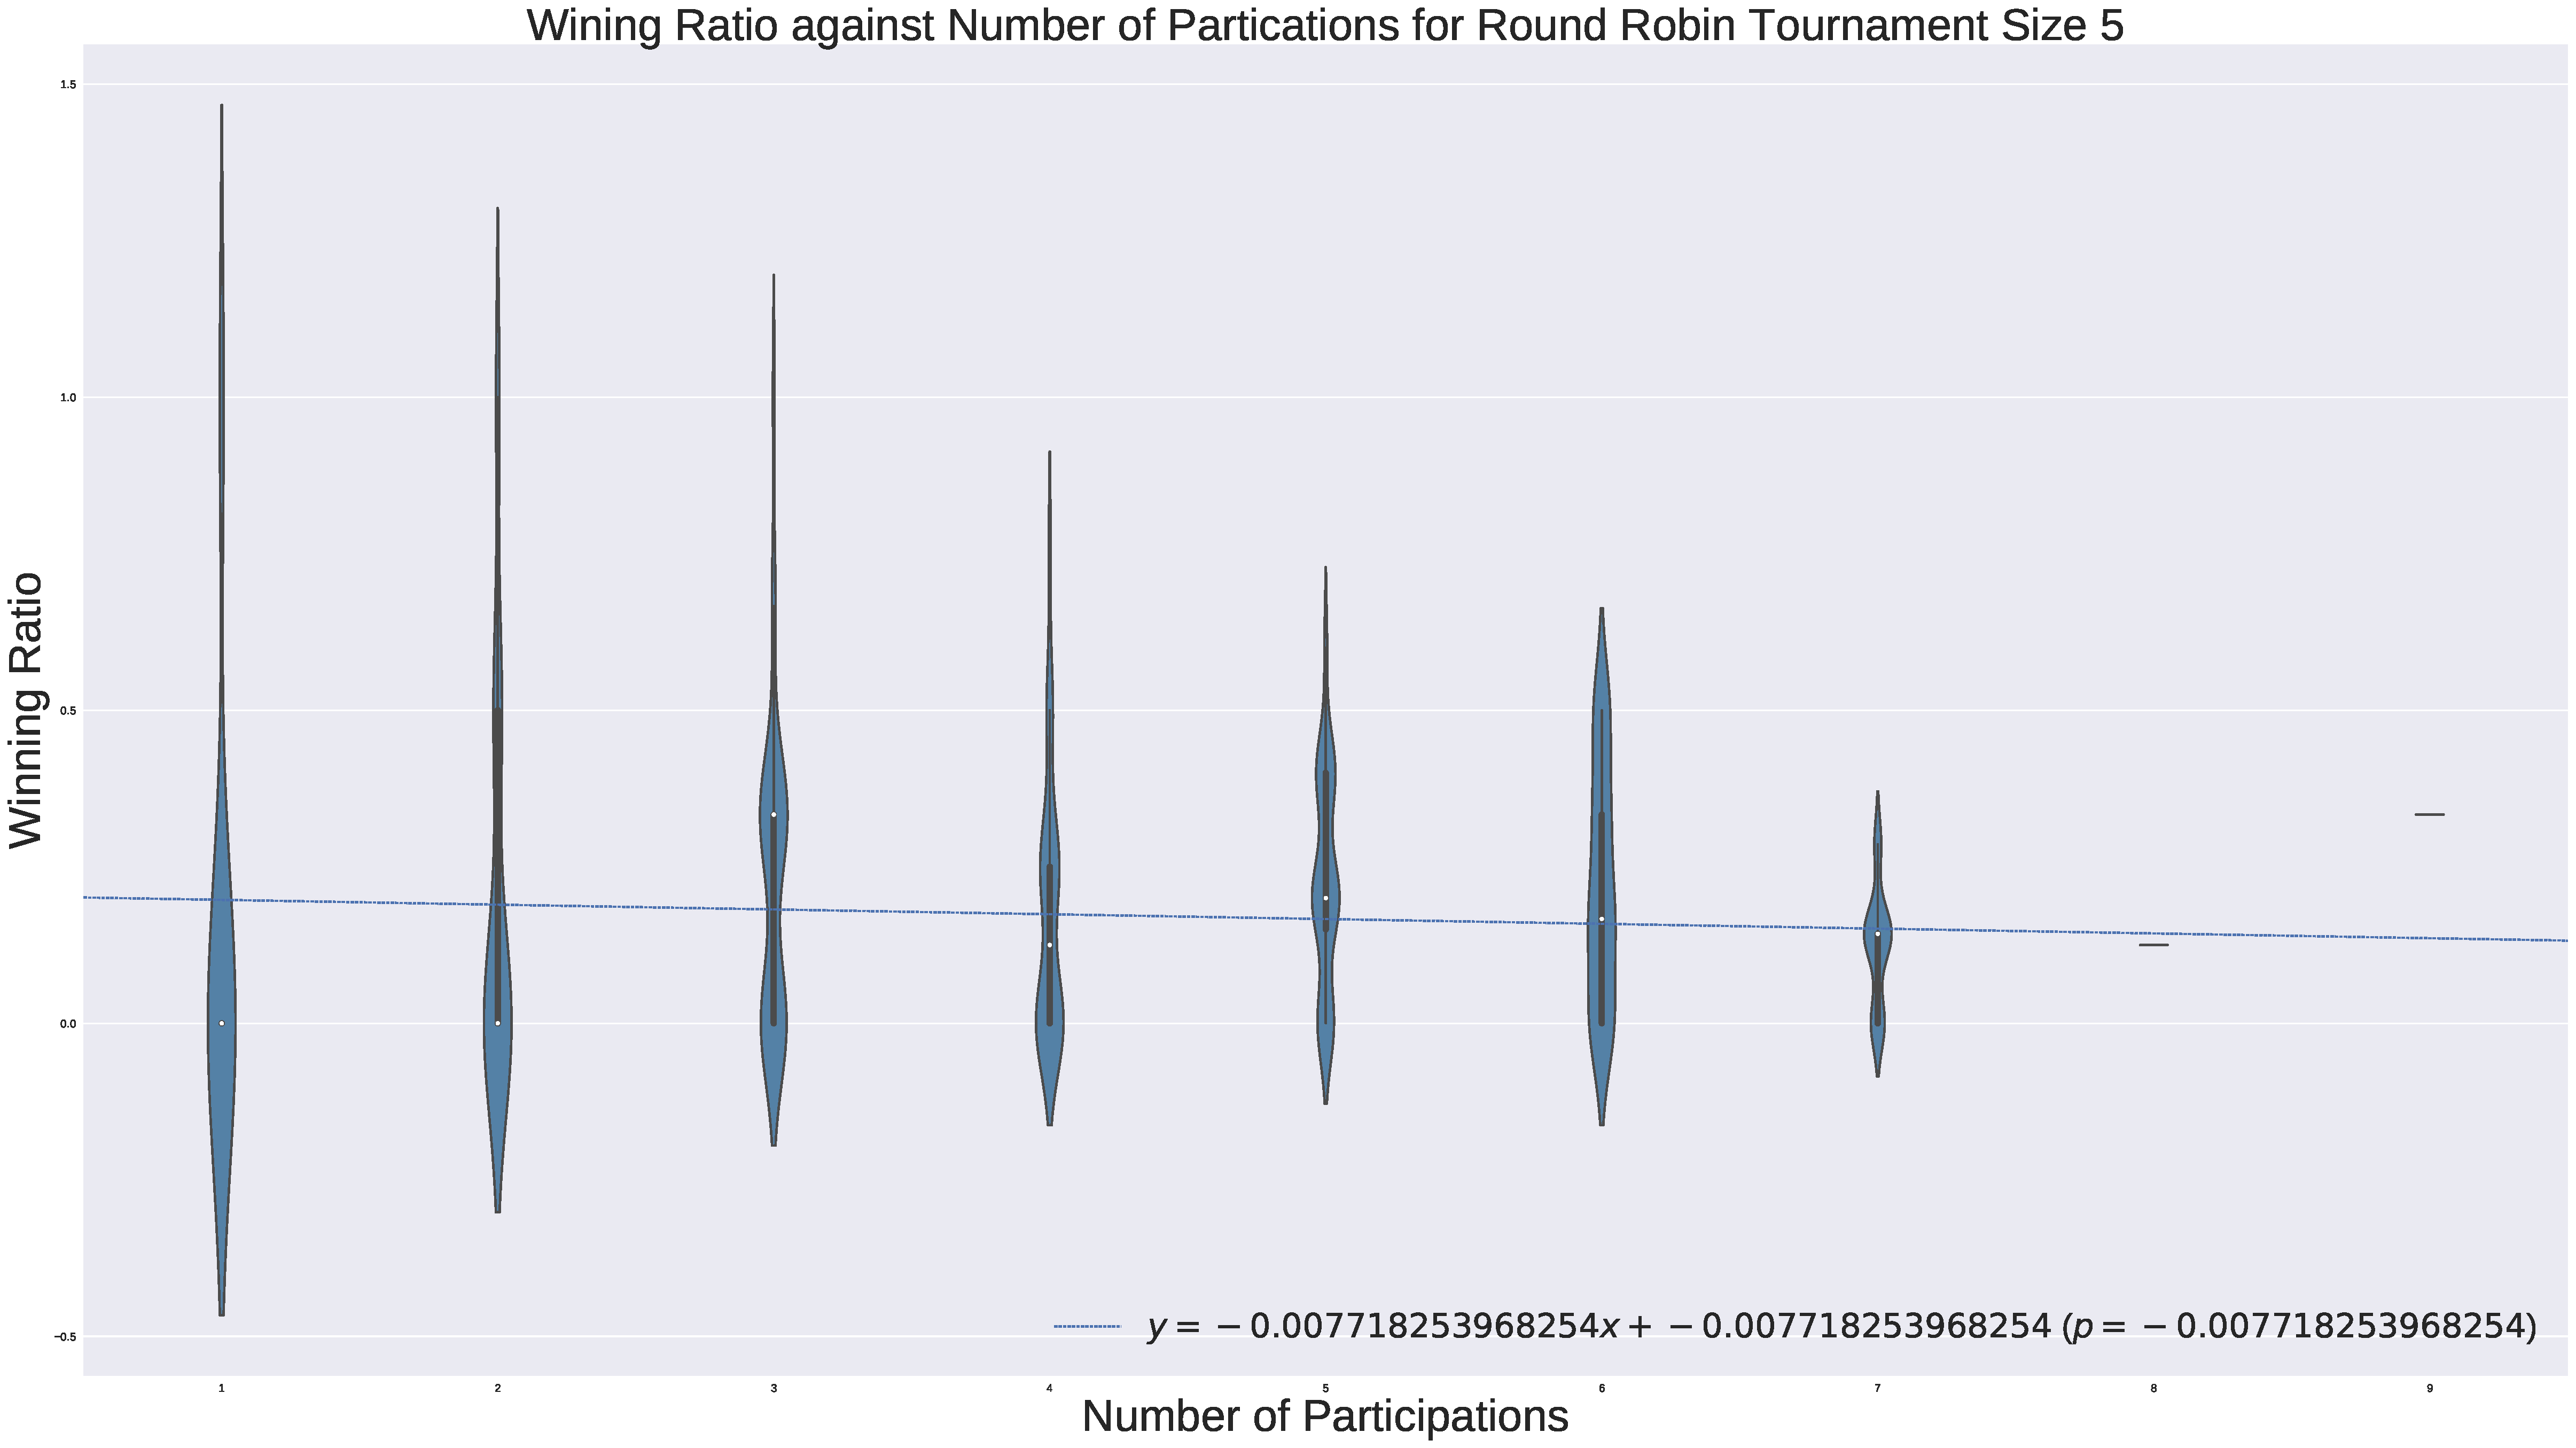
\includegraphics[width=\linewidth]{chapter-three/anova-Round-Robin-5.pdf}
		\caption{Winning ratio vs number of participations round robin tournament size 5}
	\end{subfigure}
	\caption{Winning ratio vs number of participations tournaments size 5}
	\label{fig:winning-ratio-participations-five}
\end{figure}

\begin{figure}[H]
	\centering

	\begin{subfigure}[t]{0.75\textwidth}
		\centering
		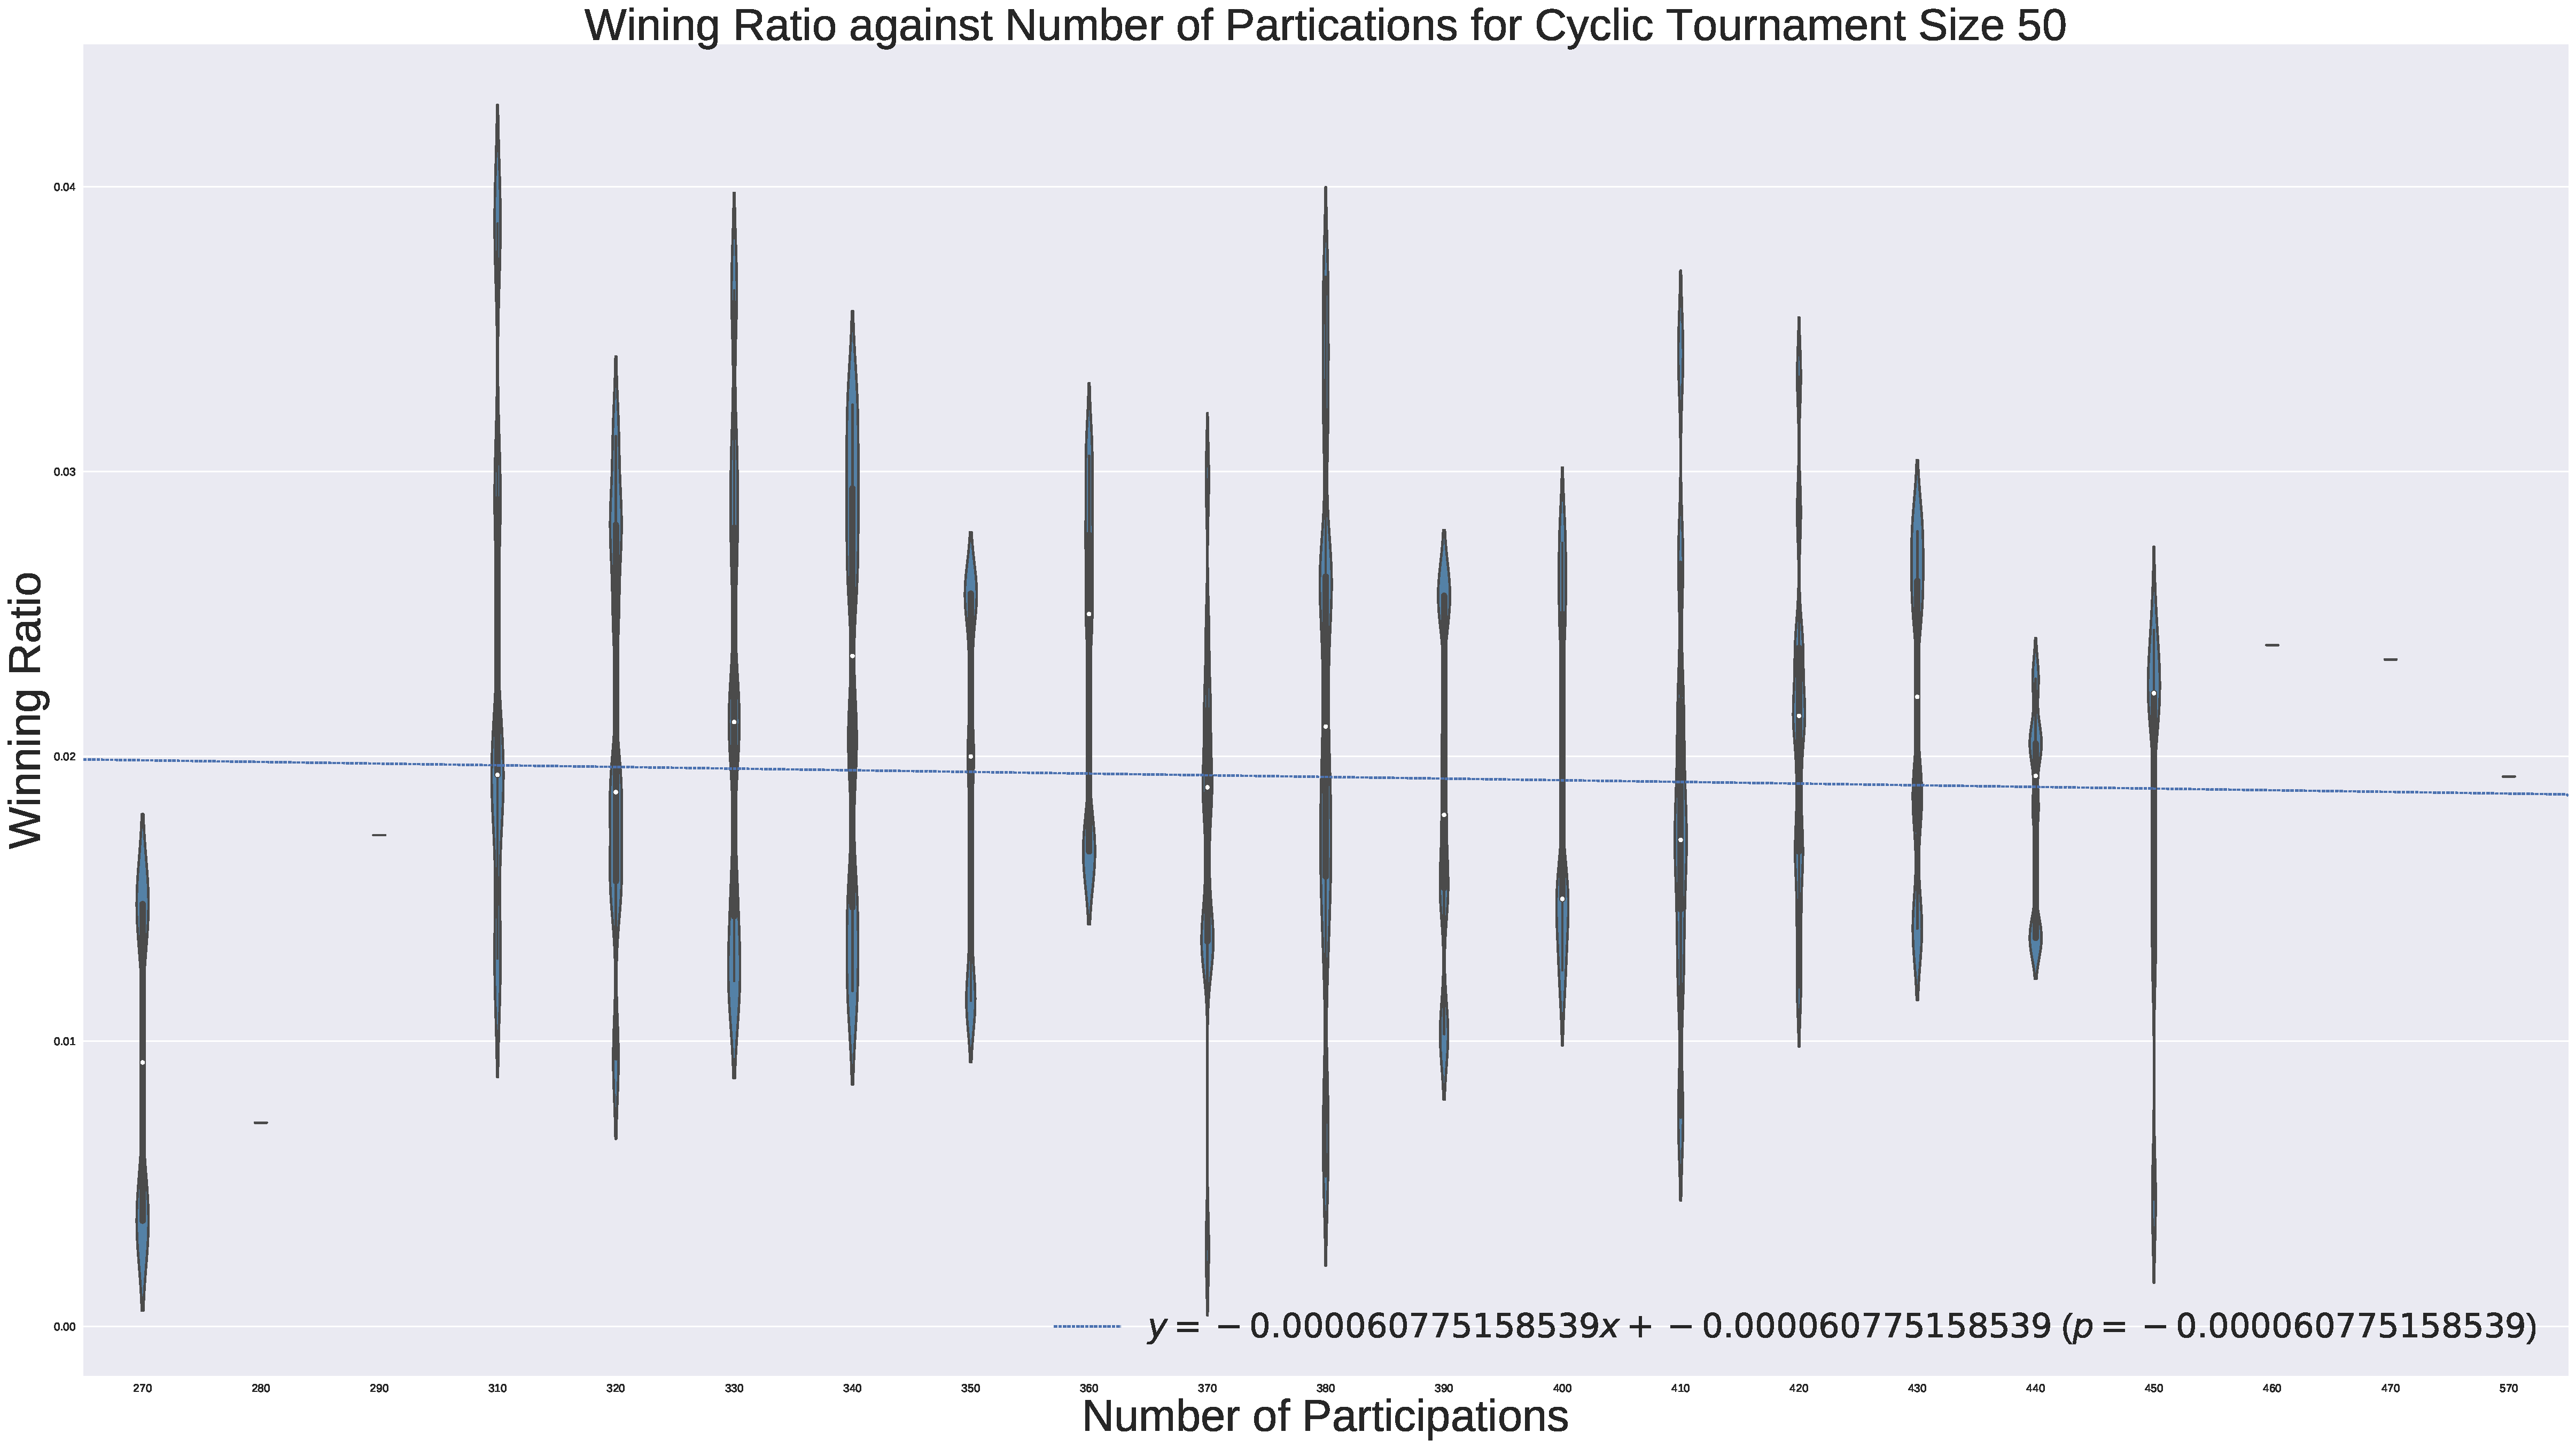
\includegraphics[width=\linewidth]{chapter-three/anova-Cyclic-50.pdf}
		\caption{Winning ratio vs number of participations cyclic tournament size 50}
	\end{subfigure}
	\hfill
	\begin{subfigure}[t]{0.75\textwidth}\centering
		\centering
		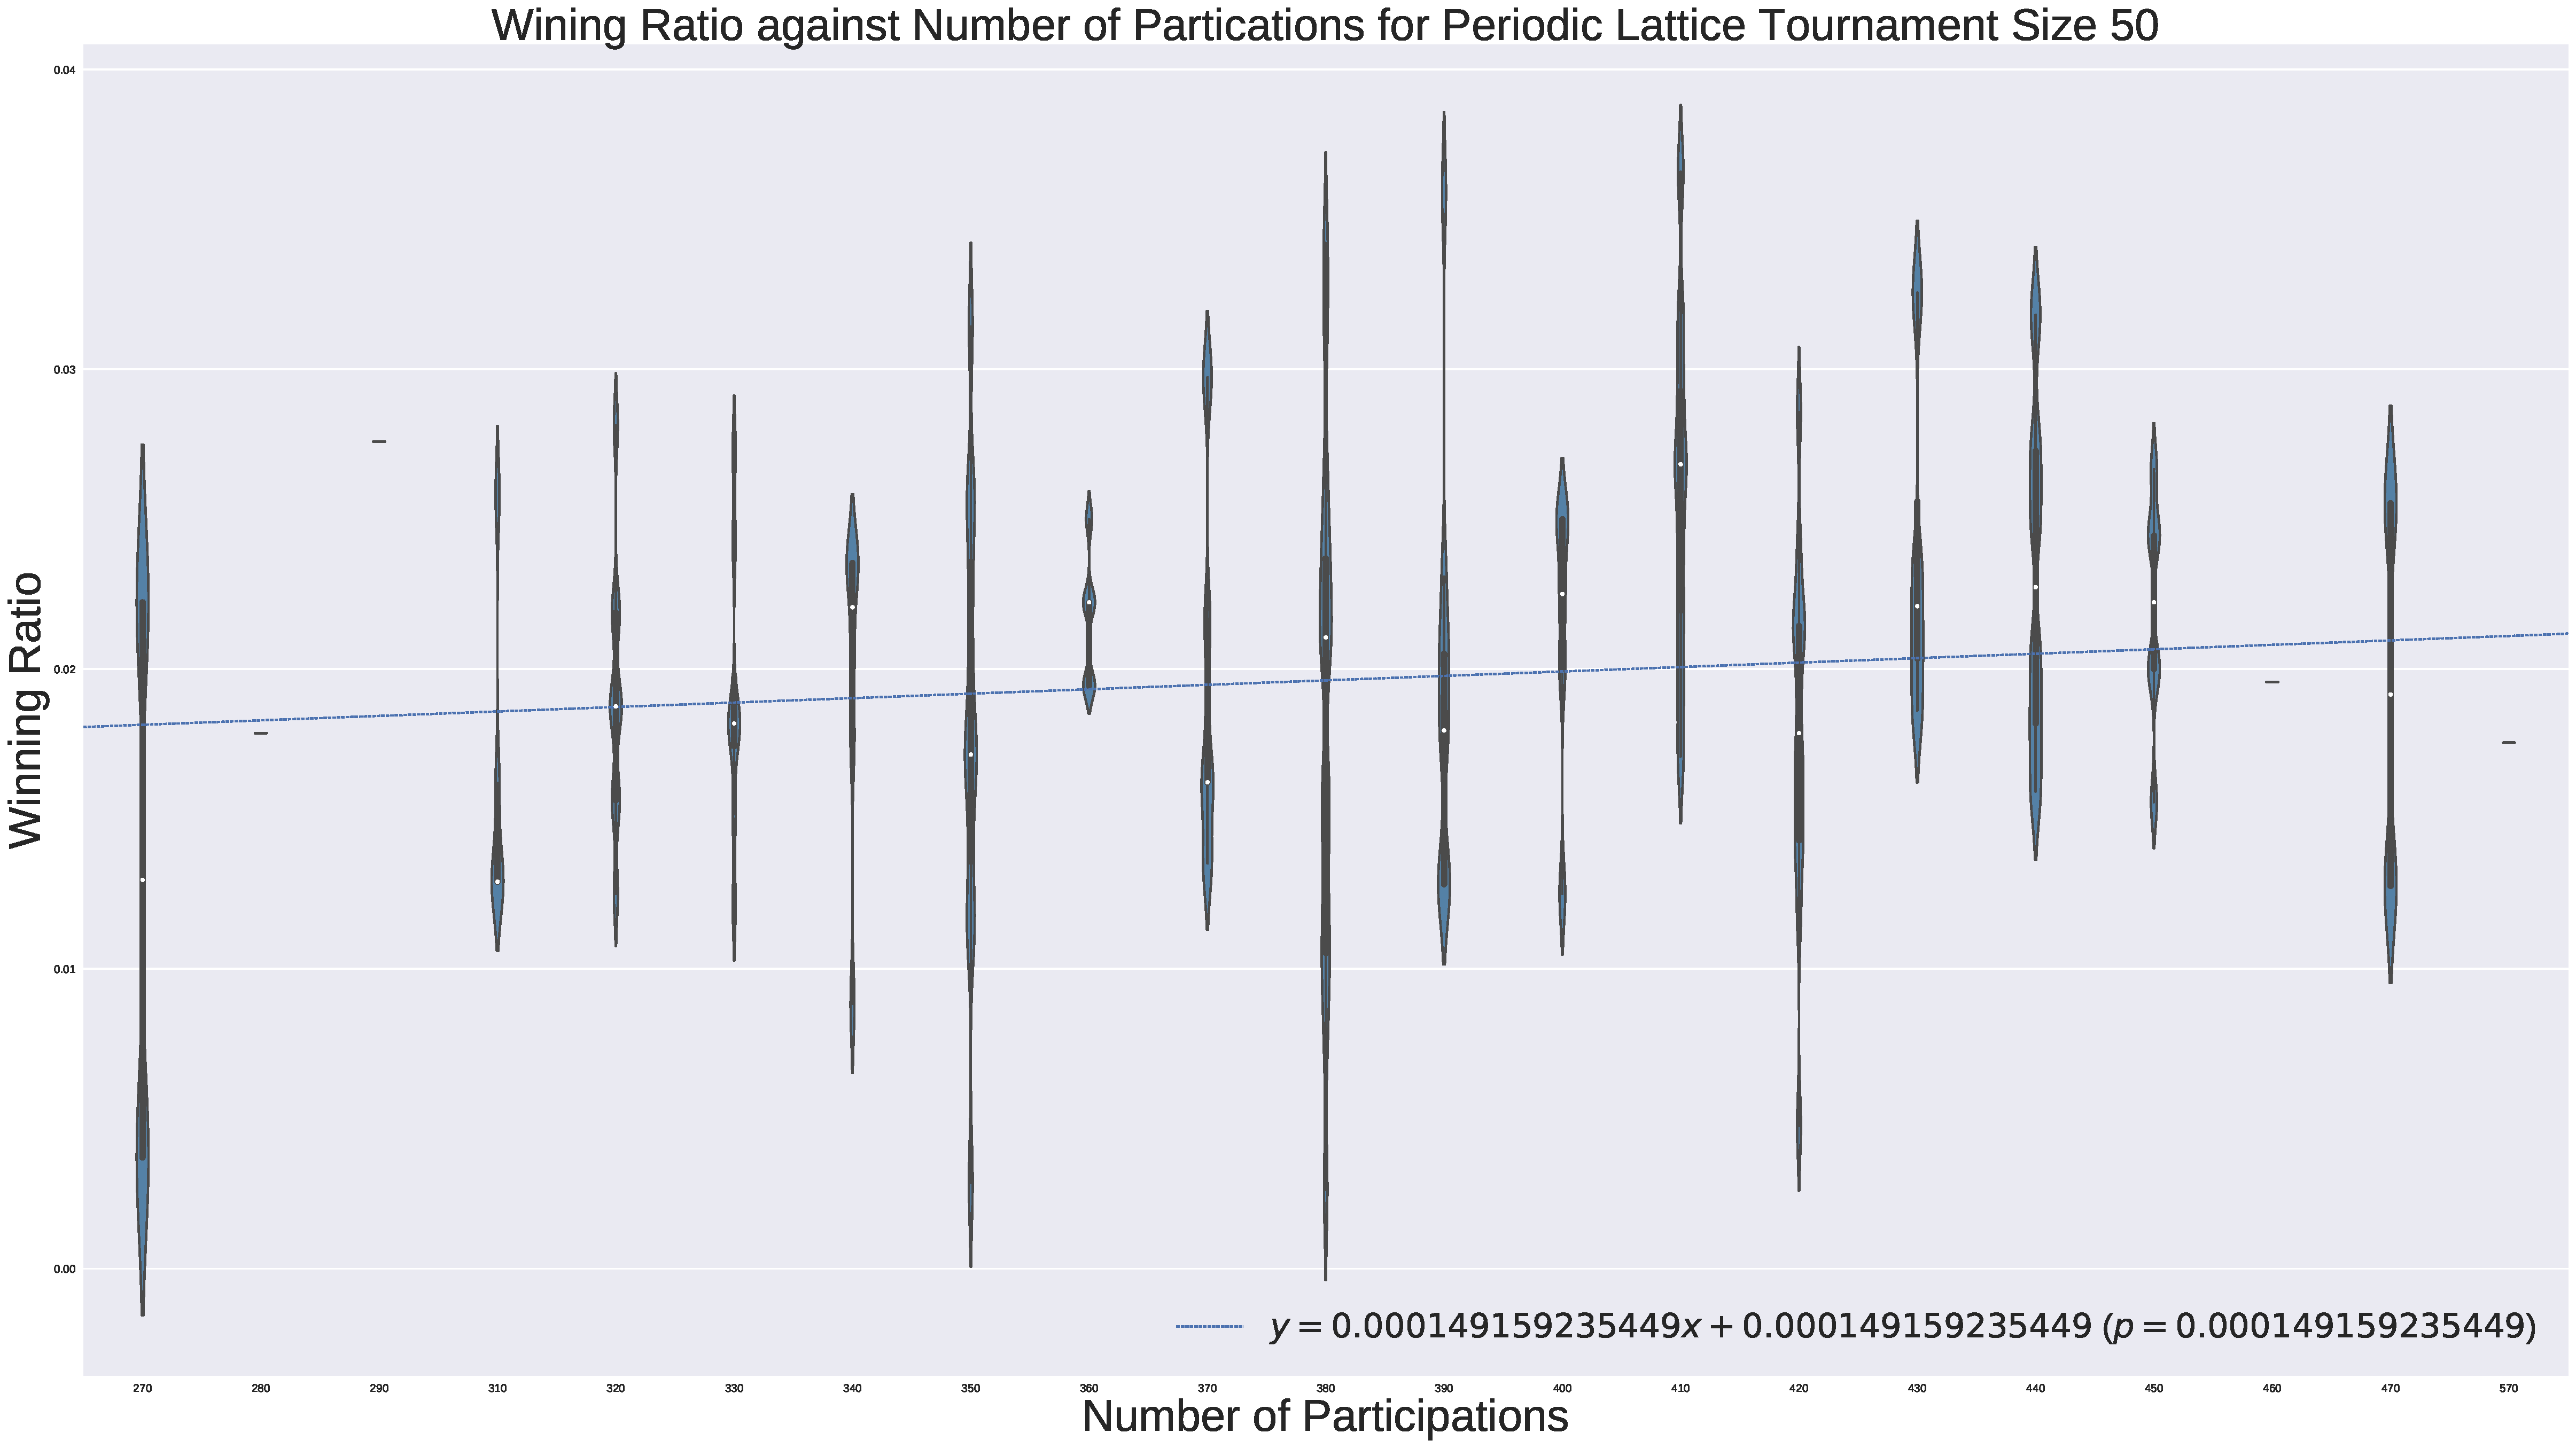
\includegraphics[width=\linewidth]{chapter-three/anova-Periodic-Lattice-50.pdf}
		\caption{Winning ratio vs number of participations periodic lattice tournament size 50}
	\end{subfigure}
	\hfill
	\begin{subfigure}[t]{0.75\textwidth}\centering
		\centering
		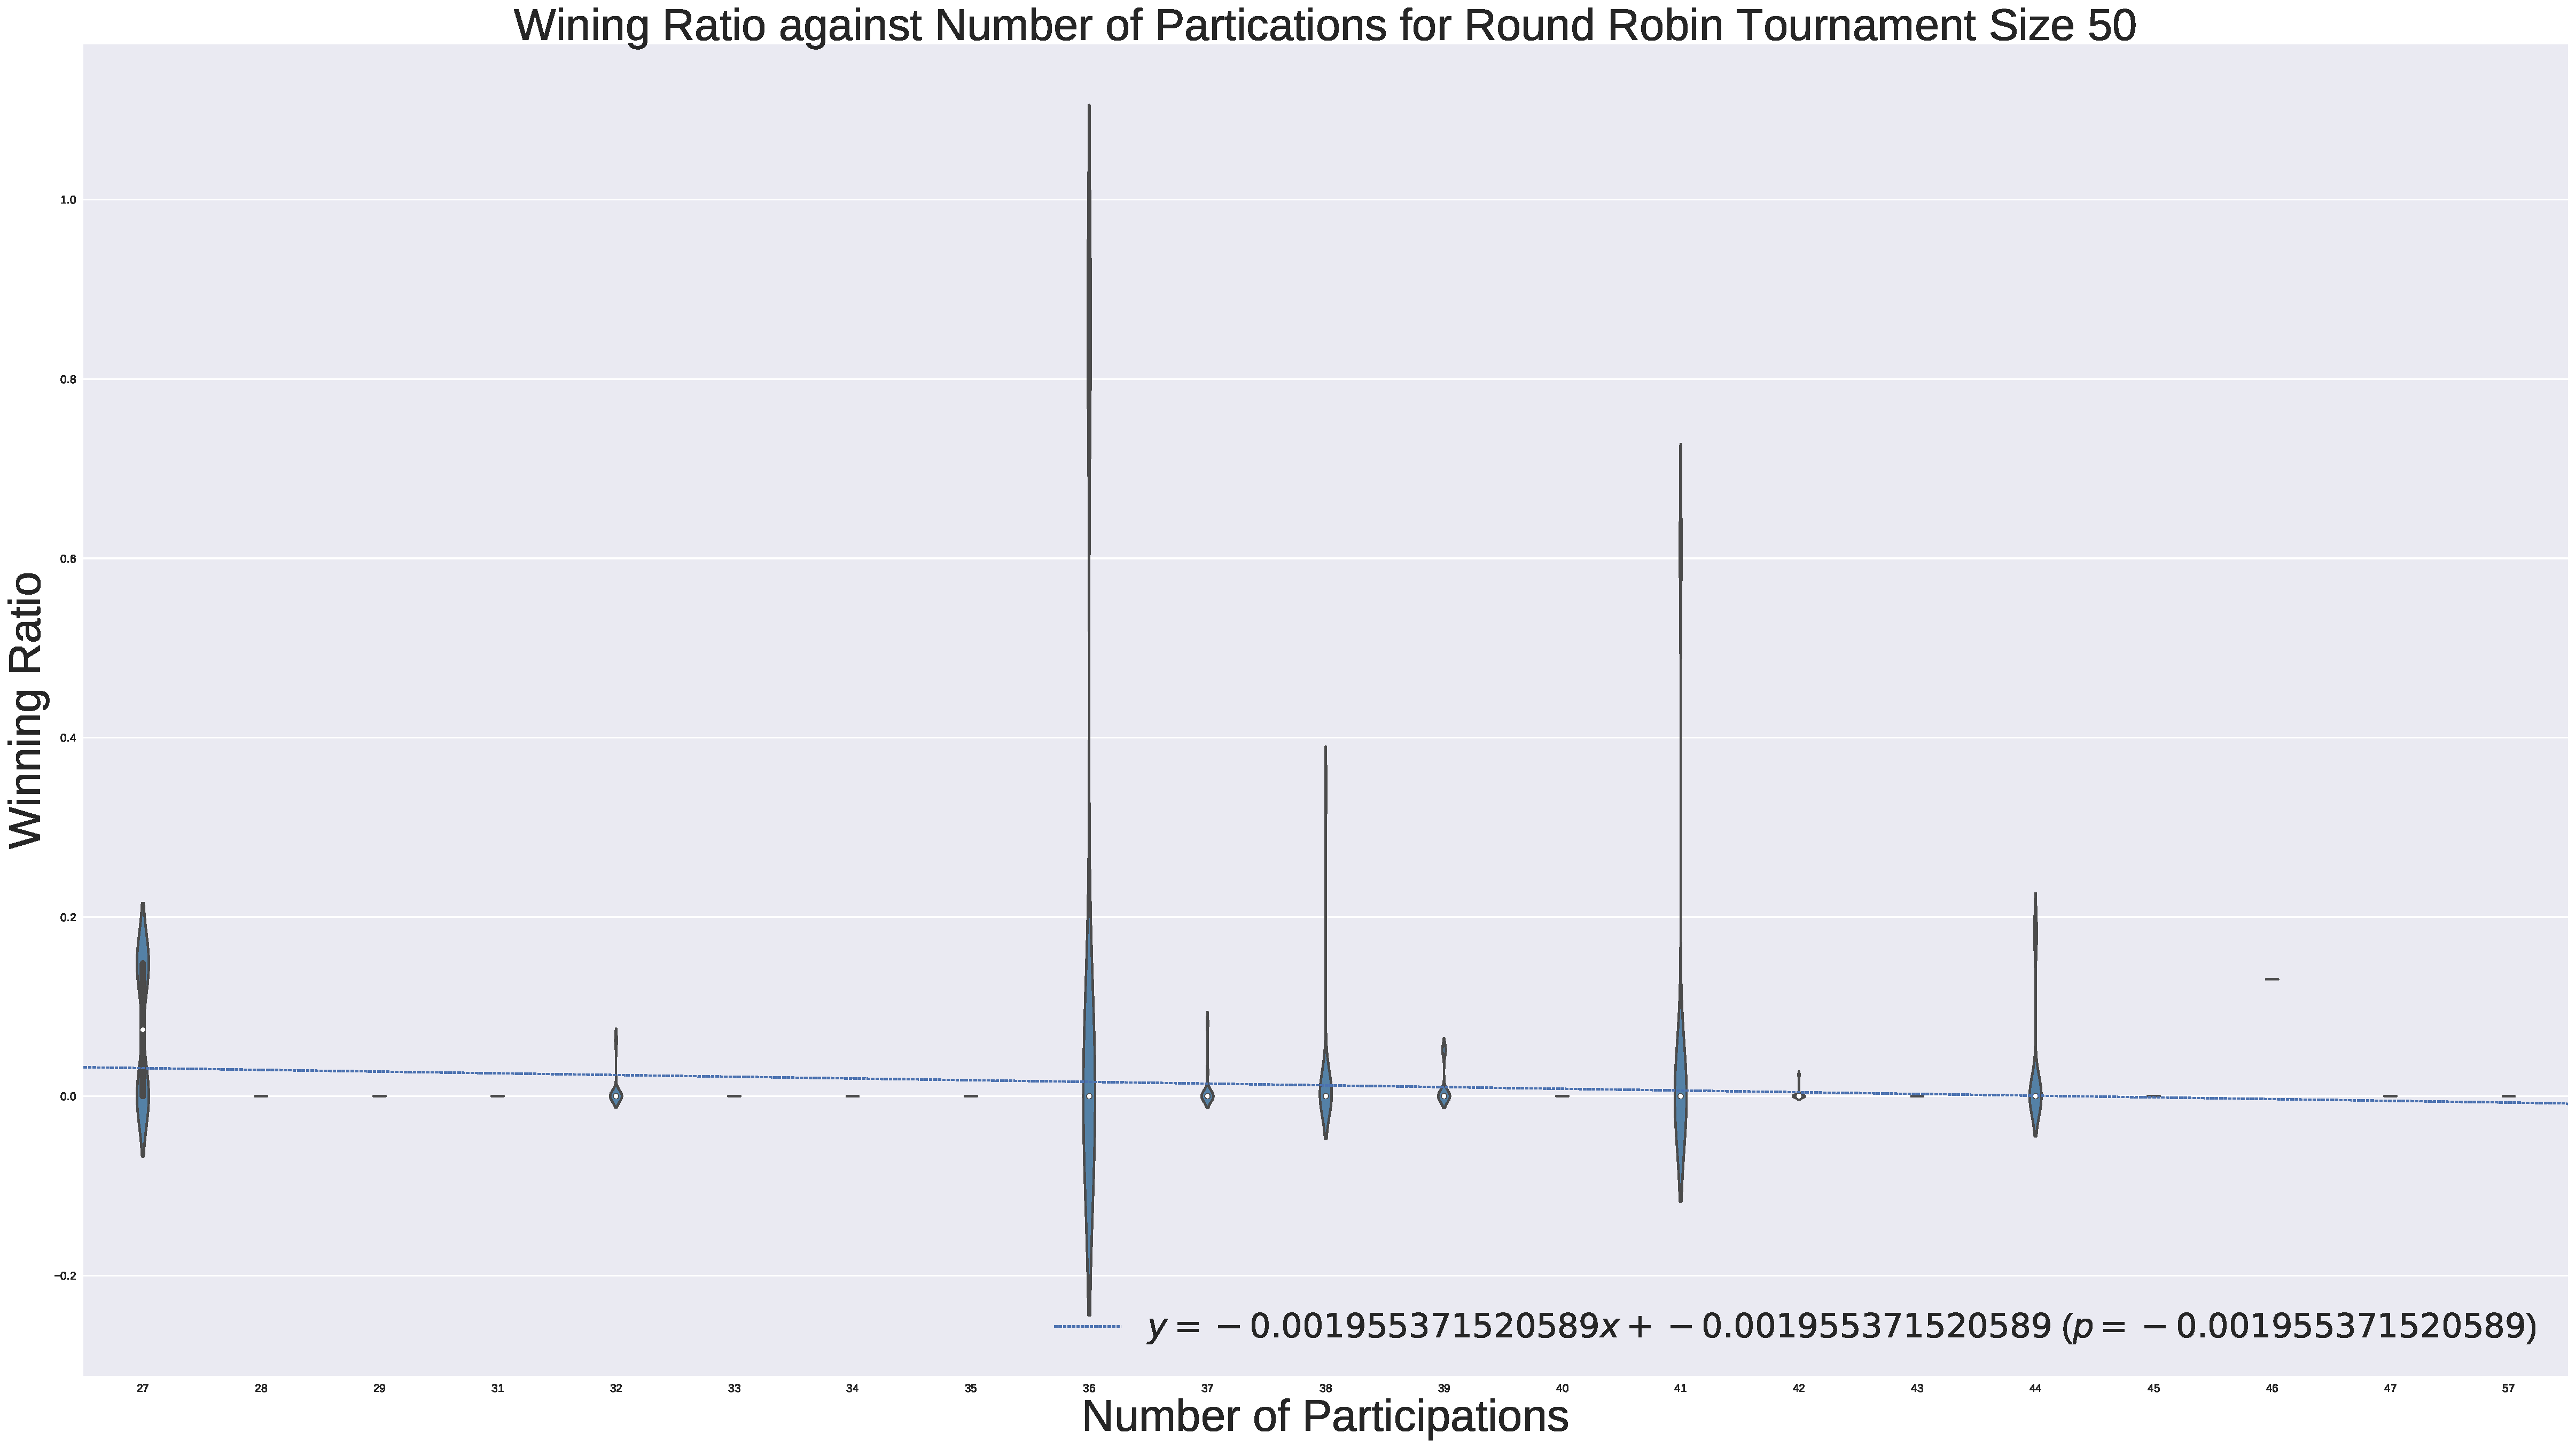
\includegraphics[width=\linewidth]{chapter-three/anova-Round-Robin-50.pdf}
		\caption{Winning ratio vs number of participations round robin tournament size 50}
	\end{subfigure}
	\caption{Winning ratio vs number of participations tournaments size 50.}
	\label{fig:winning-ratio-participations-fifty}
\end{figure}

In this subsection the winning ratio has been covered. The strategies were ranked
based on their winning ratio in each of the six experiments. Line plots that
illustrate the devolution in the strategies rankings, were conducted. Indicating
that Raider could be an overall well performing strategy. Even though, it was
not necessarily ranked first every time, it does rank highly in most experiments.

Additionally, the effect of participation frequency in the winning ratio, for
all strategies, have been investigated. The results showed a non significant
correlation of winning ratio and participation. In the next subsection, the
normalized average score achieved by the strategies will be investigated.

\subsection{Normalized Average Scores}
\label{sub:normalized_av_score}
The normalized average score is calculated by dividing the average score per
turn per opponent of each strategy with their participation counts. The variation
of the normalized average score, for each topology, has been studied and plotted.
The plots can be found in the Appendix~\ref{append:variation-plots}. A normality
test has been held, and the score is not normally distributed. Thus, a Kruskal
Wallis test has been used for the analysis.

For all six experiments the normalized average score significantly differs between
participation groups. There is a lot variation, indicating each strategy performed
differently at given points of the same experiment. These could be because of the
opponent or the whole neighborhood, a strategy was against.

The strategies, have been ranked, similarly to ~\autoref{sub:winning_ratio}, but
this time based on mean normalized average ranking. Figures \ref{fig:score-rankings-five-c-l}~\ref{fig:score-rankings-five-c-r}
~\ref{fig:score-rankings-five-l-r} and Figures~\ref{fig:score-rankings-fifty-c-l}
~\ref{fig:score-rankings-fifty-c-r}~\ref{fig:score-rankings-fifty-l-r}, illustrate
the line plots. In conclusion, for tournaments sizes 5, the top spots were dominated
by Tricky Cooperator and Raider. For tournaments sizes 50, Forgetful Fool Me Once,
and Hard Tit For 2 Tats attract attention. All this strategies, have been ranked
low in the previous subsection. Specifically, Tricky Cooperator and Hard Tit For 2 Tats,
had a winning ratio of zero for specific topologies. This is an effect, of the
strategies loosing to a well performed opponent which participates in more tournaments.
Thus, the well performed opponent's average score, divided by a bigger number
of participations, is lower.

\begin{figure}[H]
	\centering
	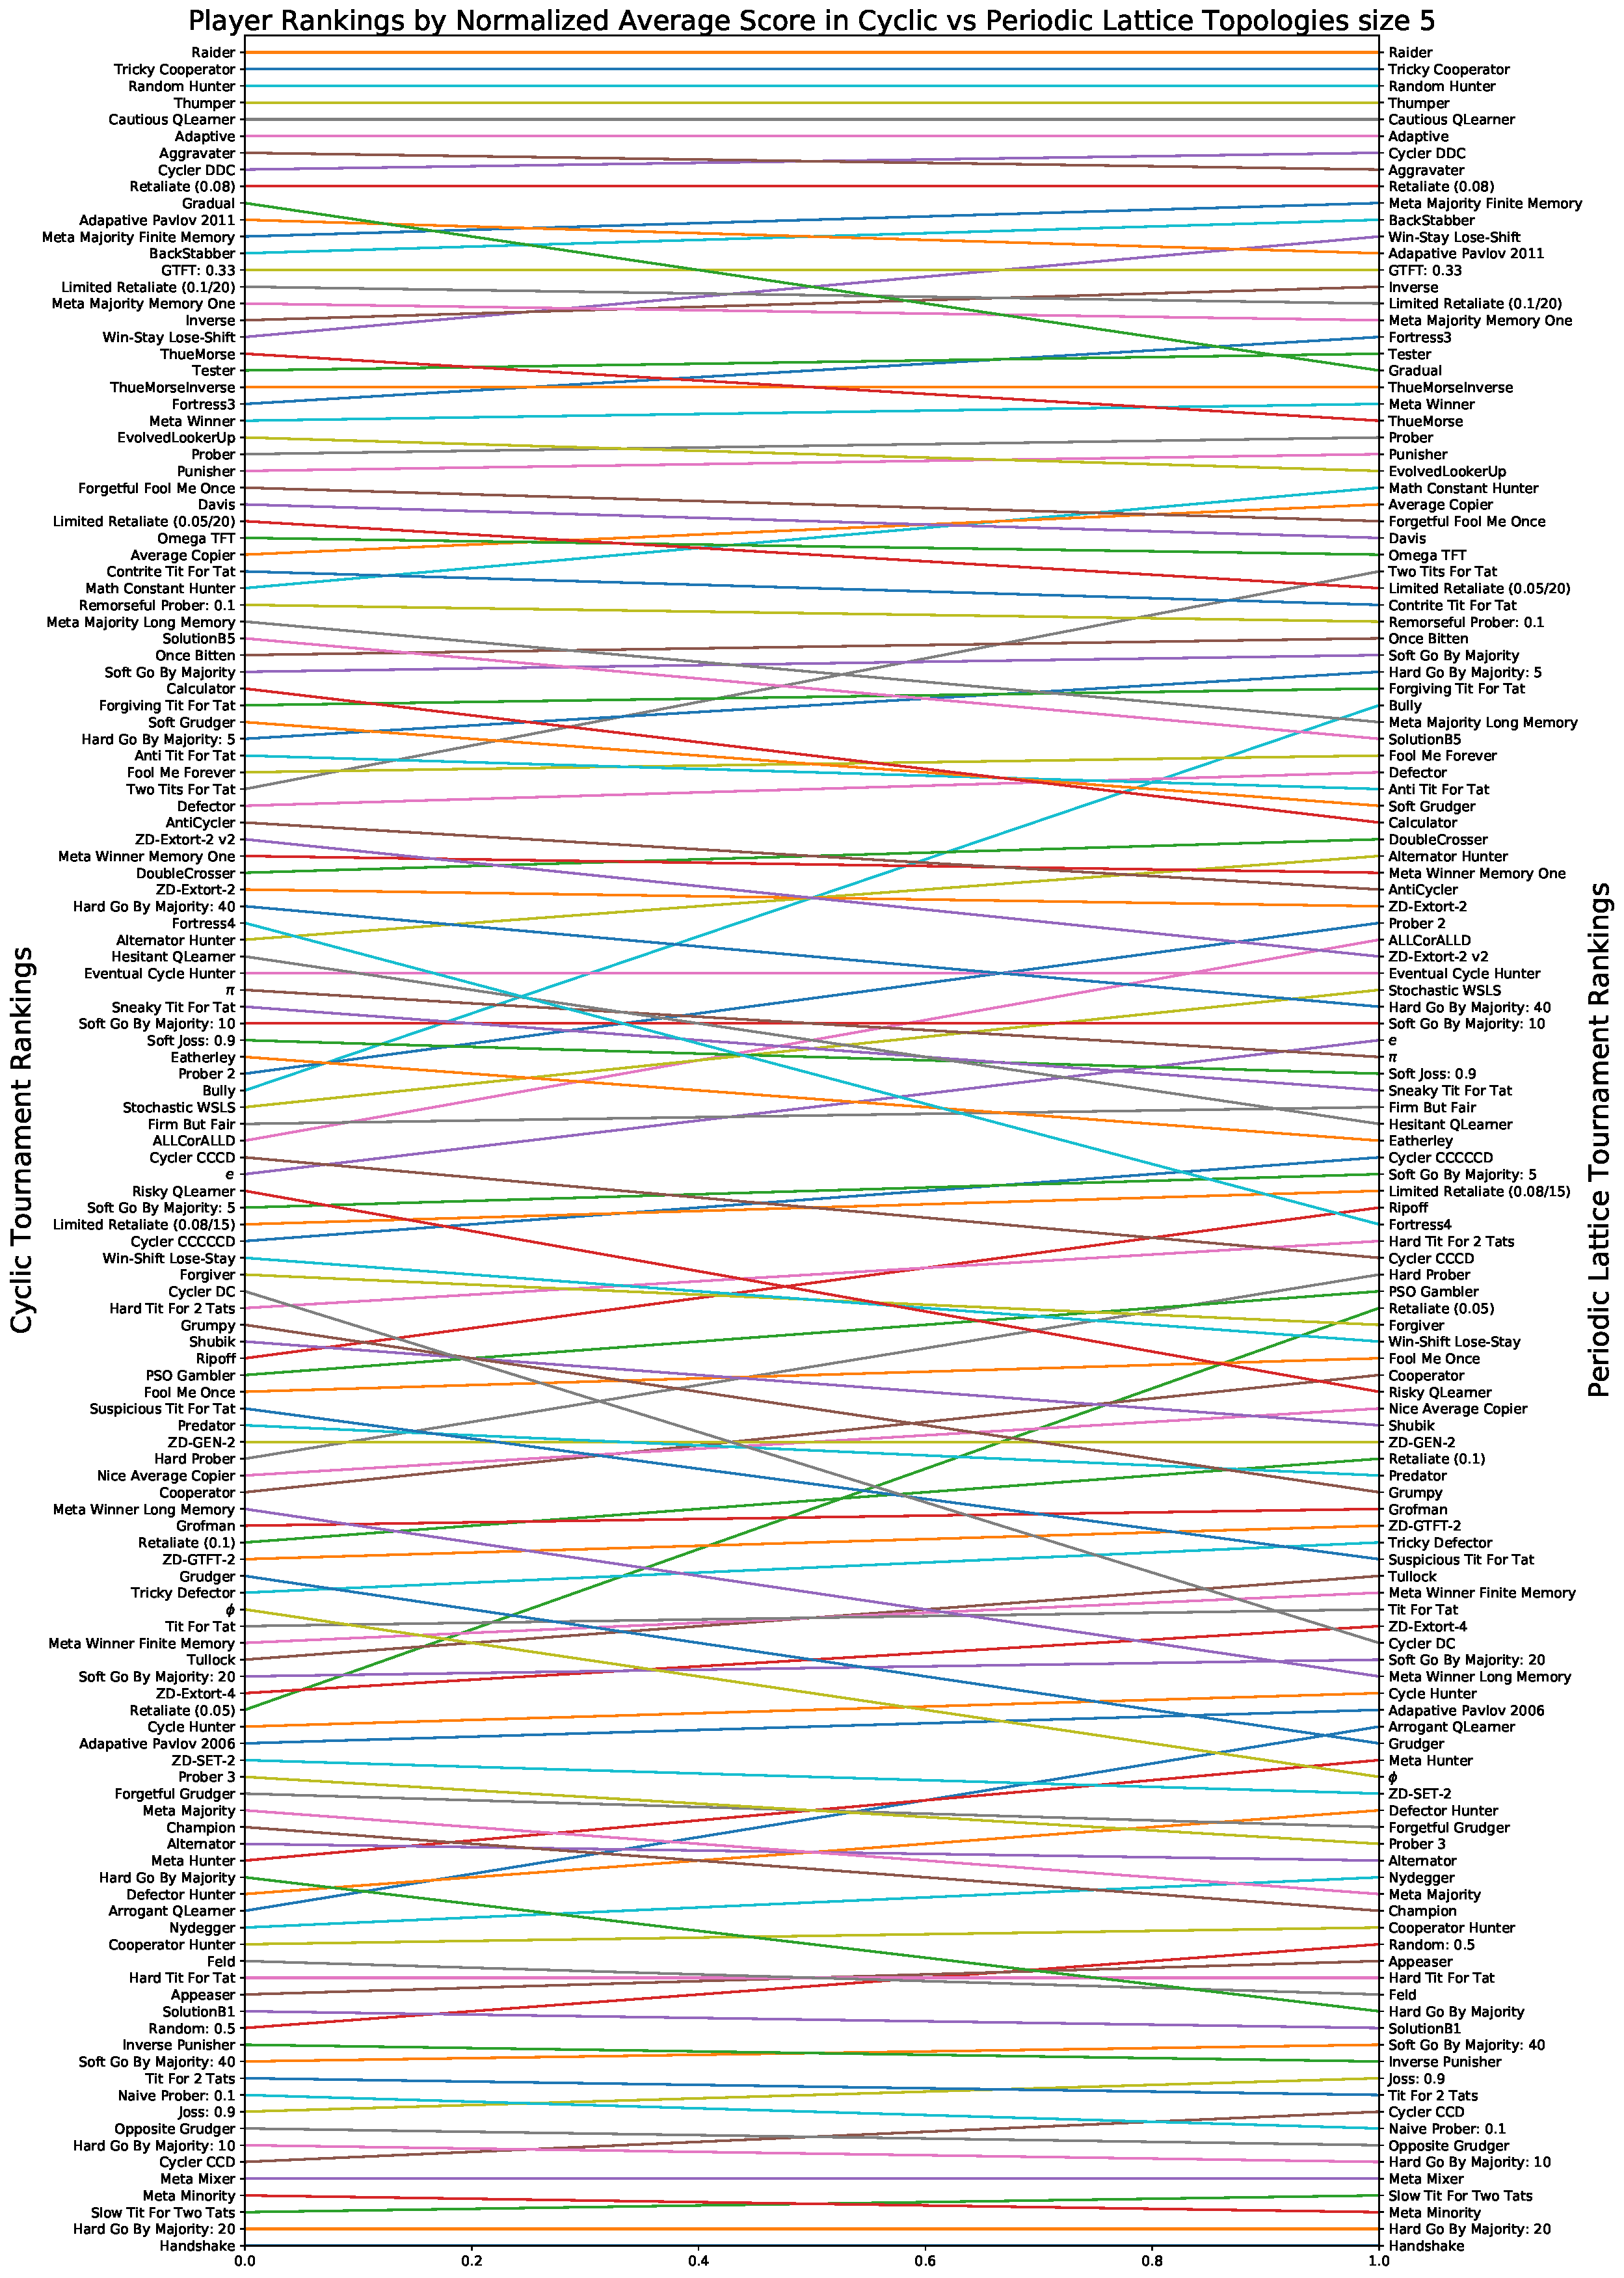
\includegraphics[width=\linewidth]{chapter-three/cyclic-lattice-5.pdf}
	\caption{Cyclic vs Periodic Lattice topologies size 5}
	\label{fig:score-rankings-five-c-l}
\end{figure}

\begin{figure}[H]
	\centering
	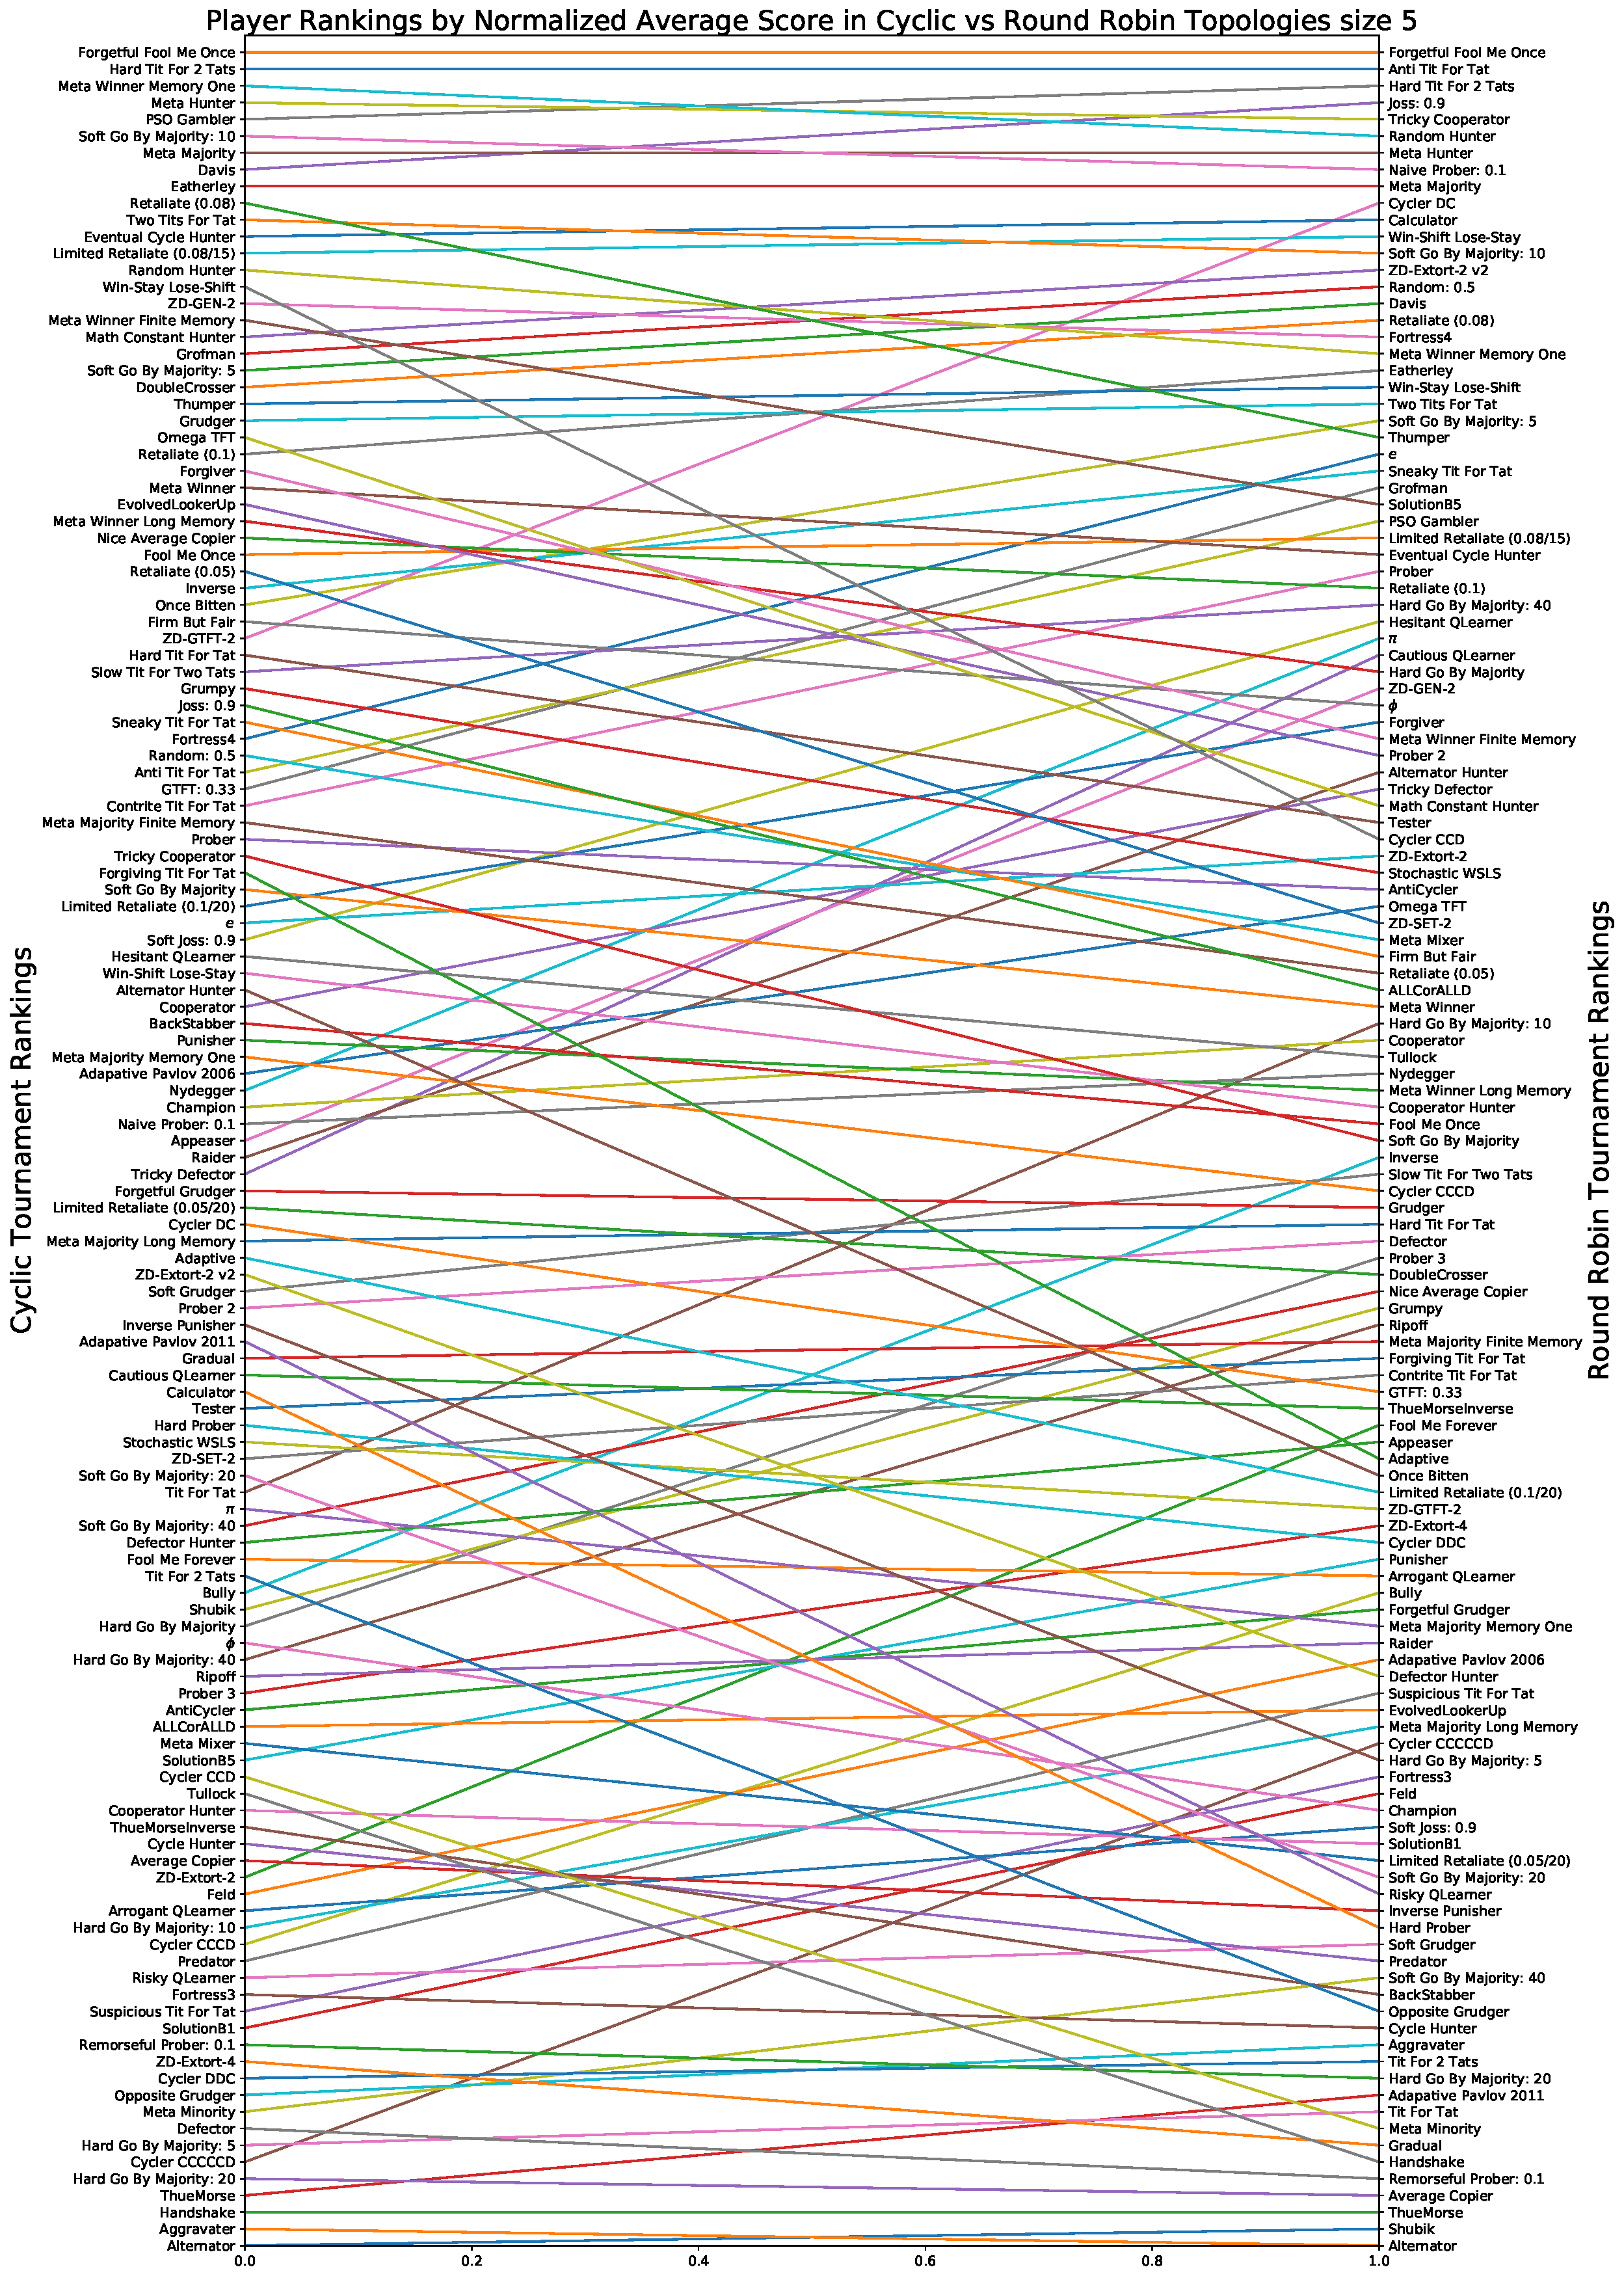
\includegraphics[width=\linewidth]{chapter-three/cyclic-round-robin-5.pdf}\
	\caption{Cyclic vs Round Robin topologies size 5}
	\label{fig:score-rankings-five-c-r}
\end{figure}

\begin{figure}[H]
	\centering
	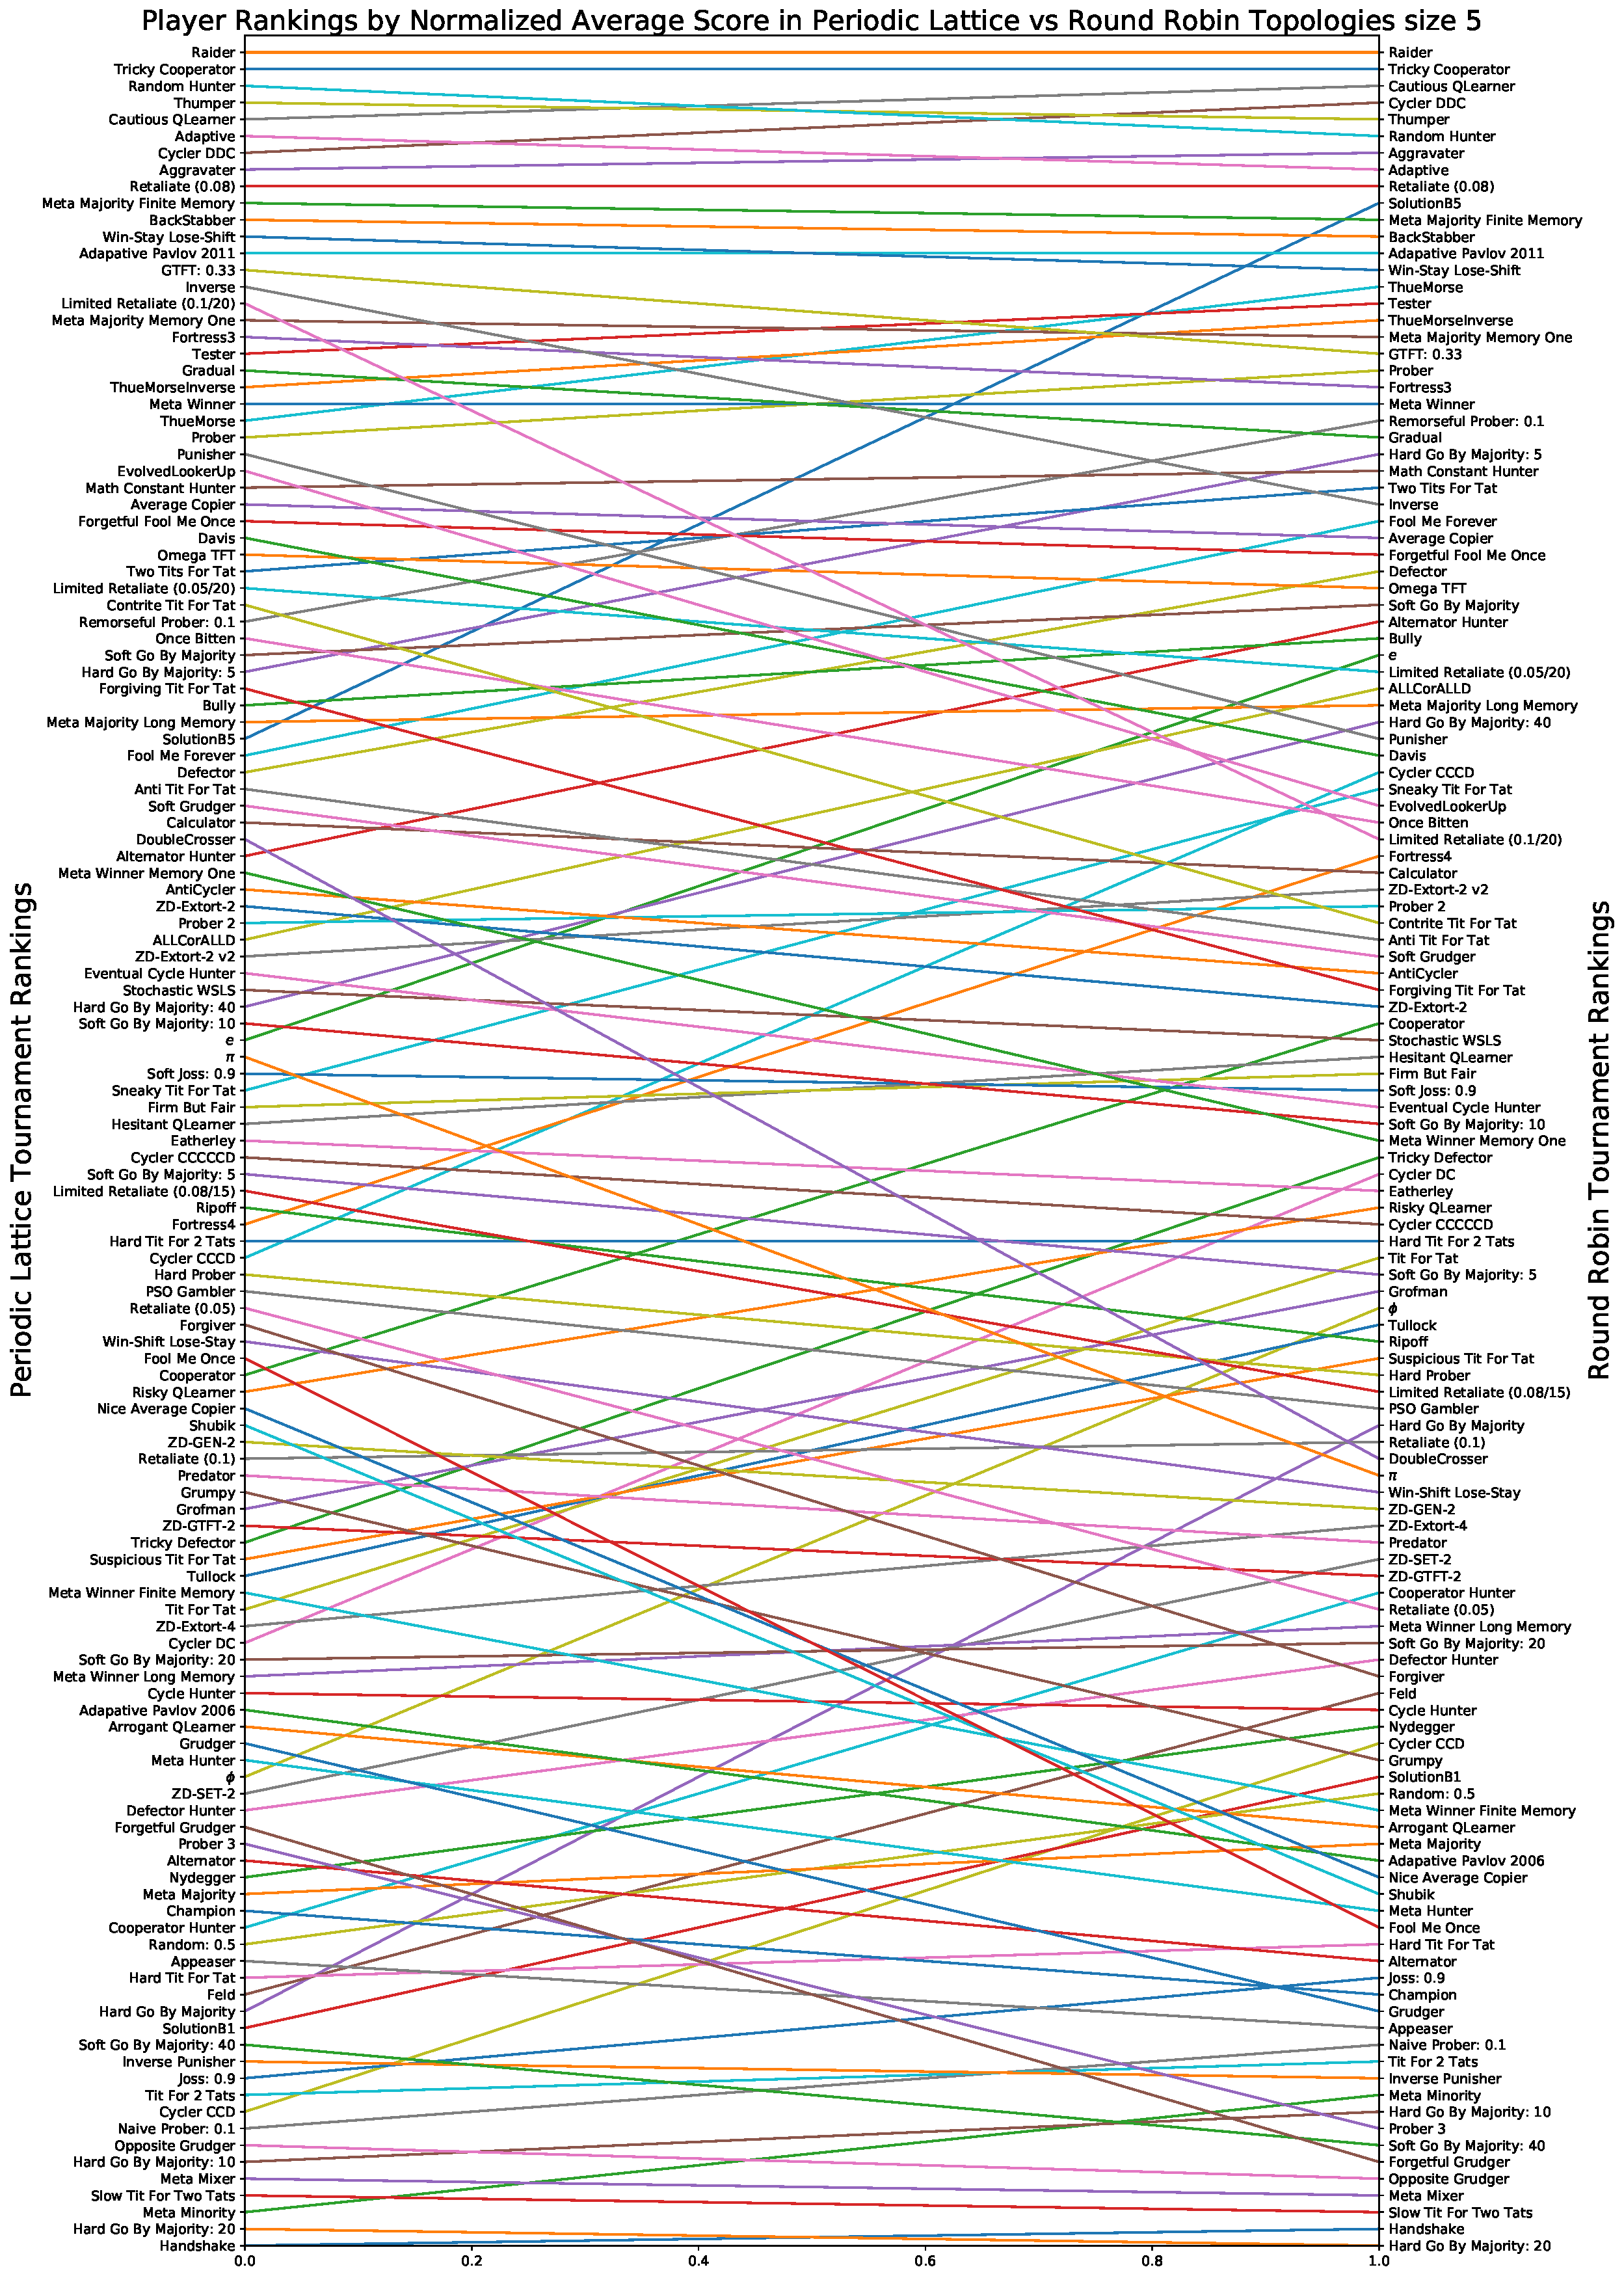
\includegraphics[width=\linewidth]{chapter-three/lattice-round-robin-5.pdf}\
	\caption{Periodic Lattice vs Round
	Robin topologies size 5}
	\label{fig:score-rankings-five-l-r}
\end{figure}

\begin{figure}[H]
	\centering
	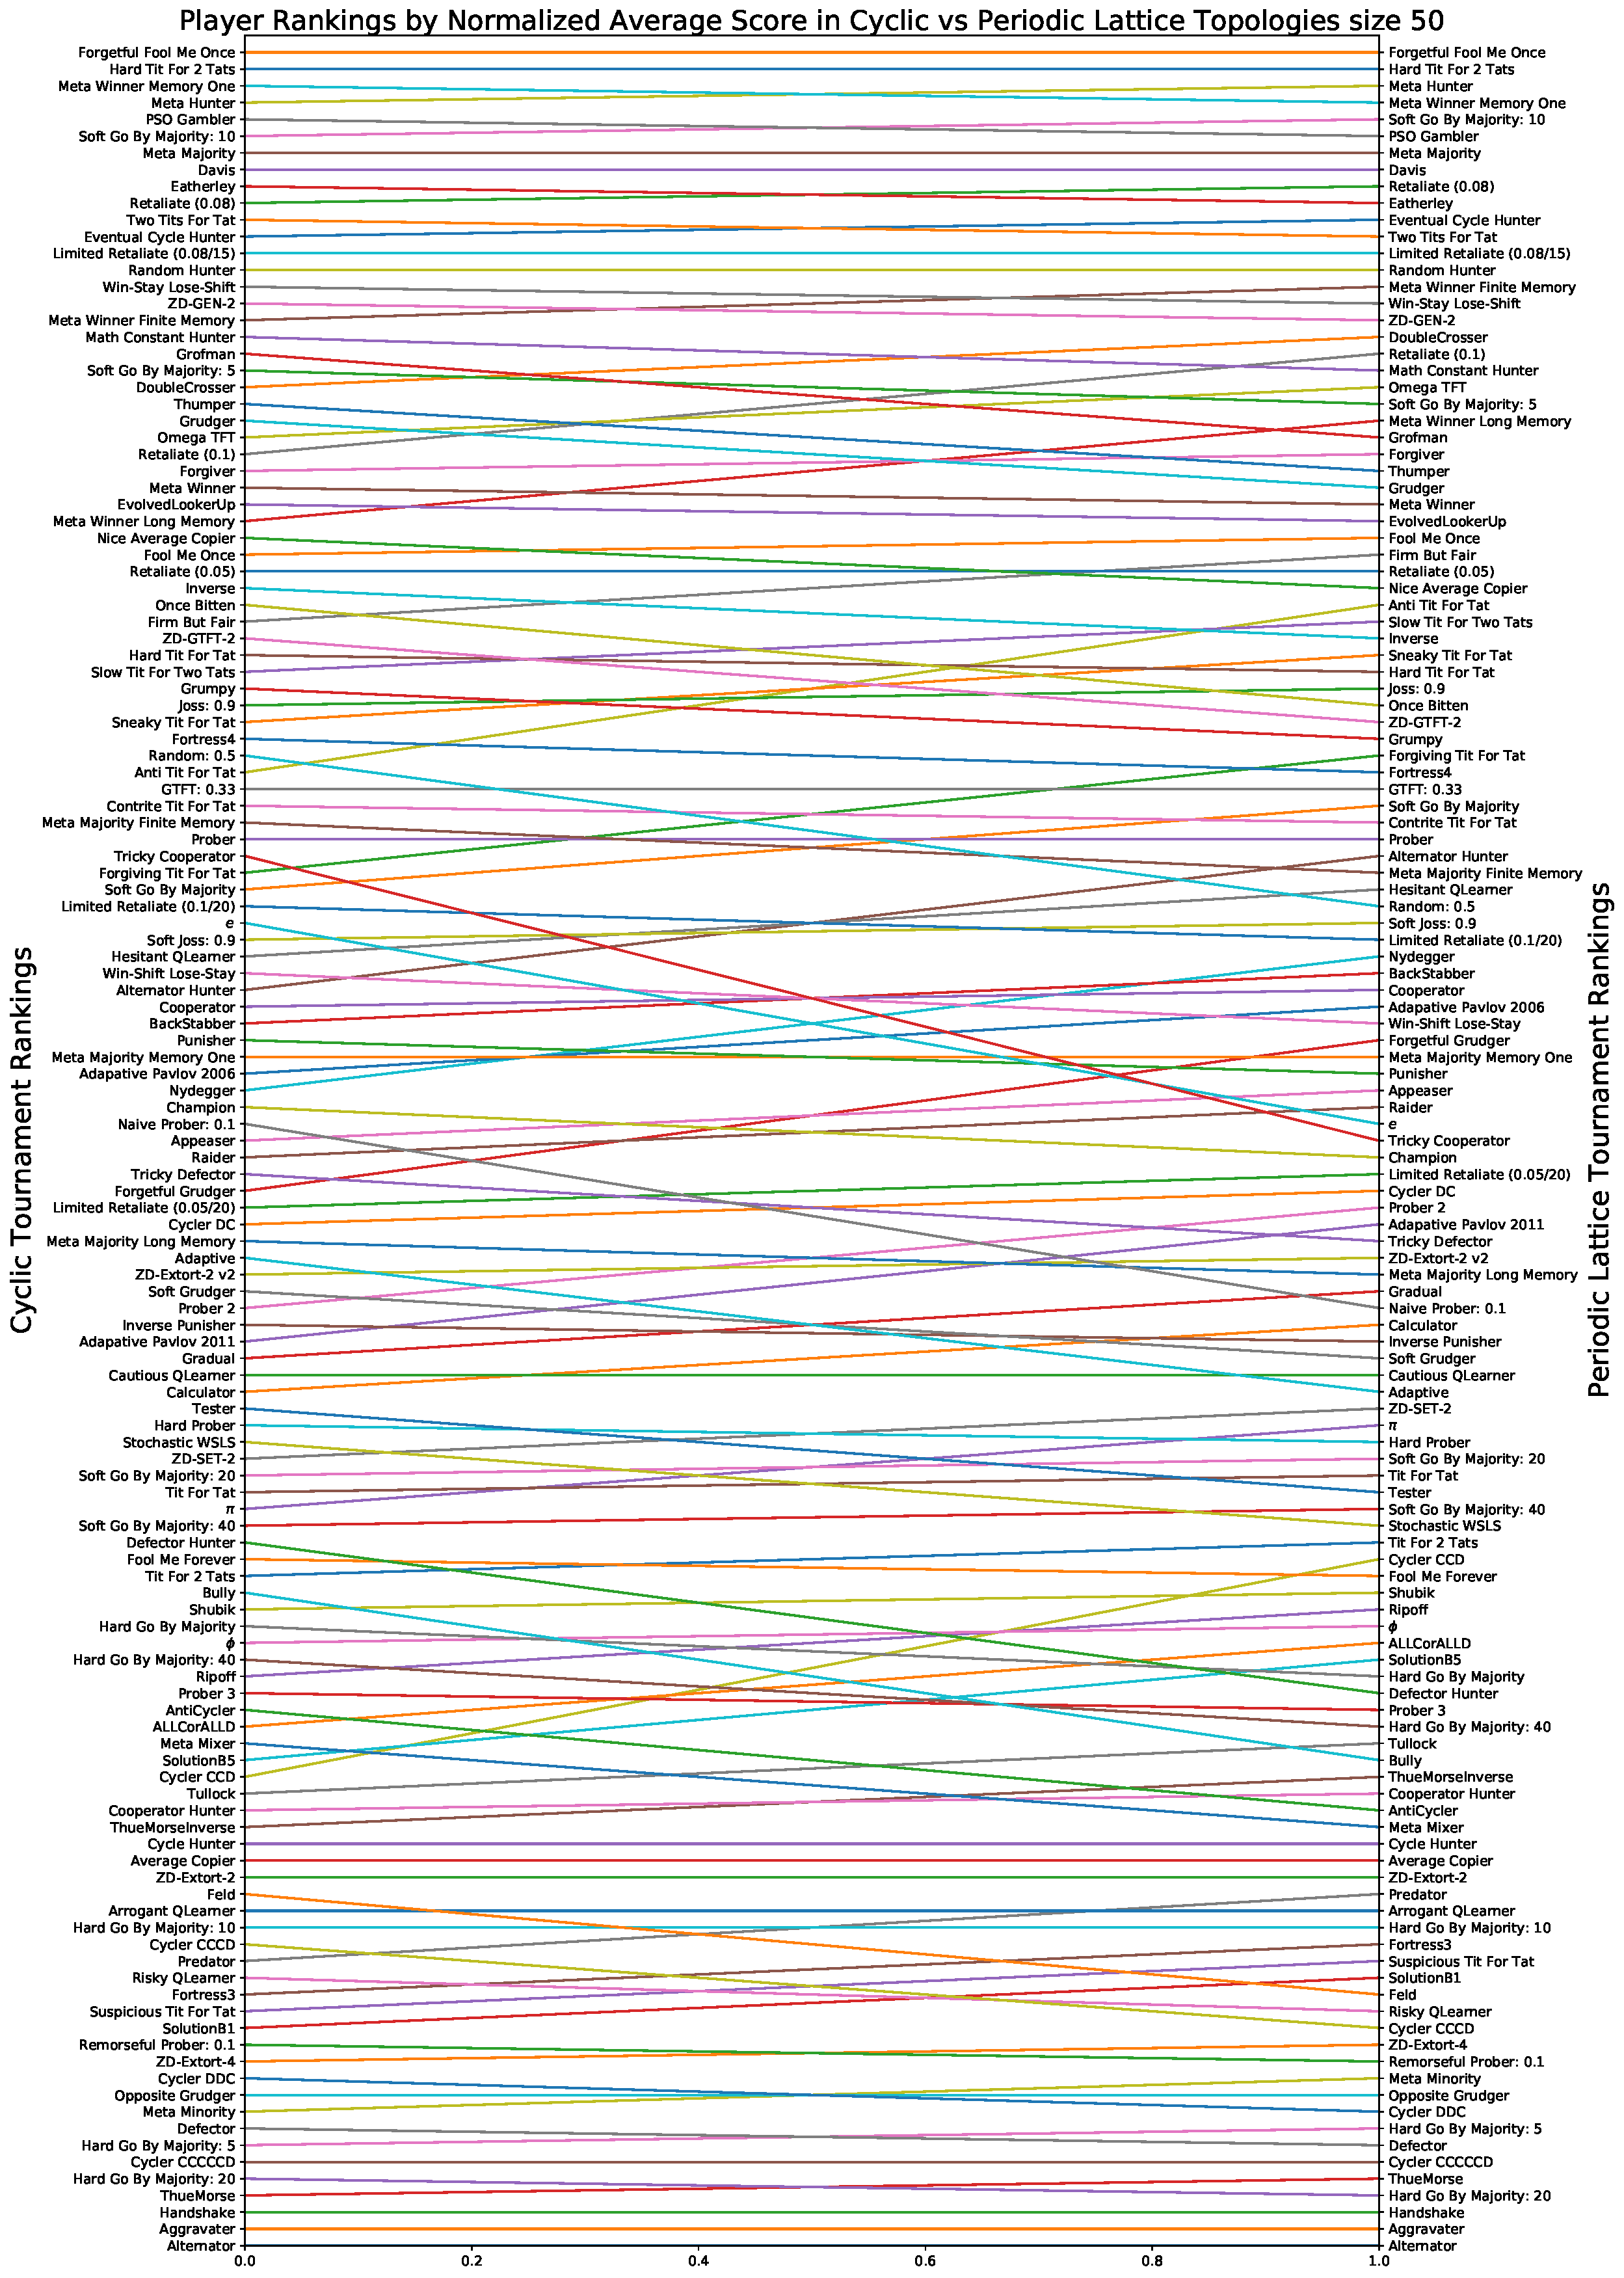
\includegraphics[width=\linewidth]{chapter-three/cyclic-lattice-50.pdf}
	\caption{Cyclic vs Periodic Lattice topologies size 50}
	\label{fig:score-rankings-fifty-c-l}
\end{figure}

\begin{figure}[H]
	\centering
	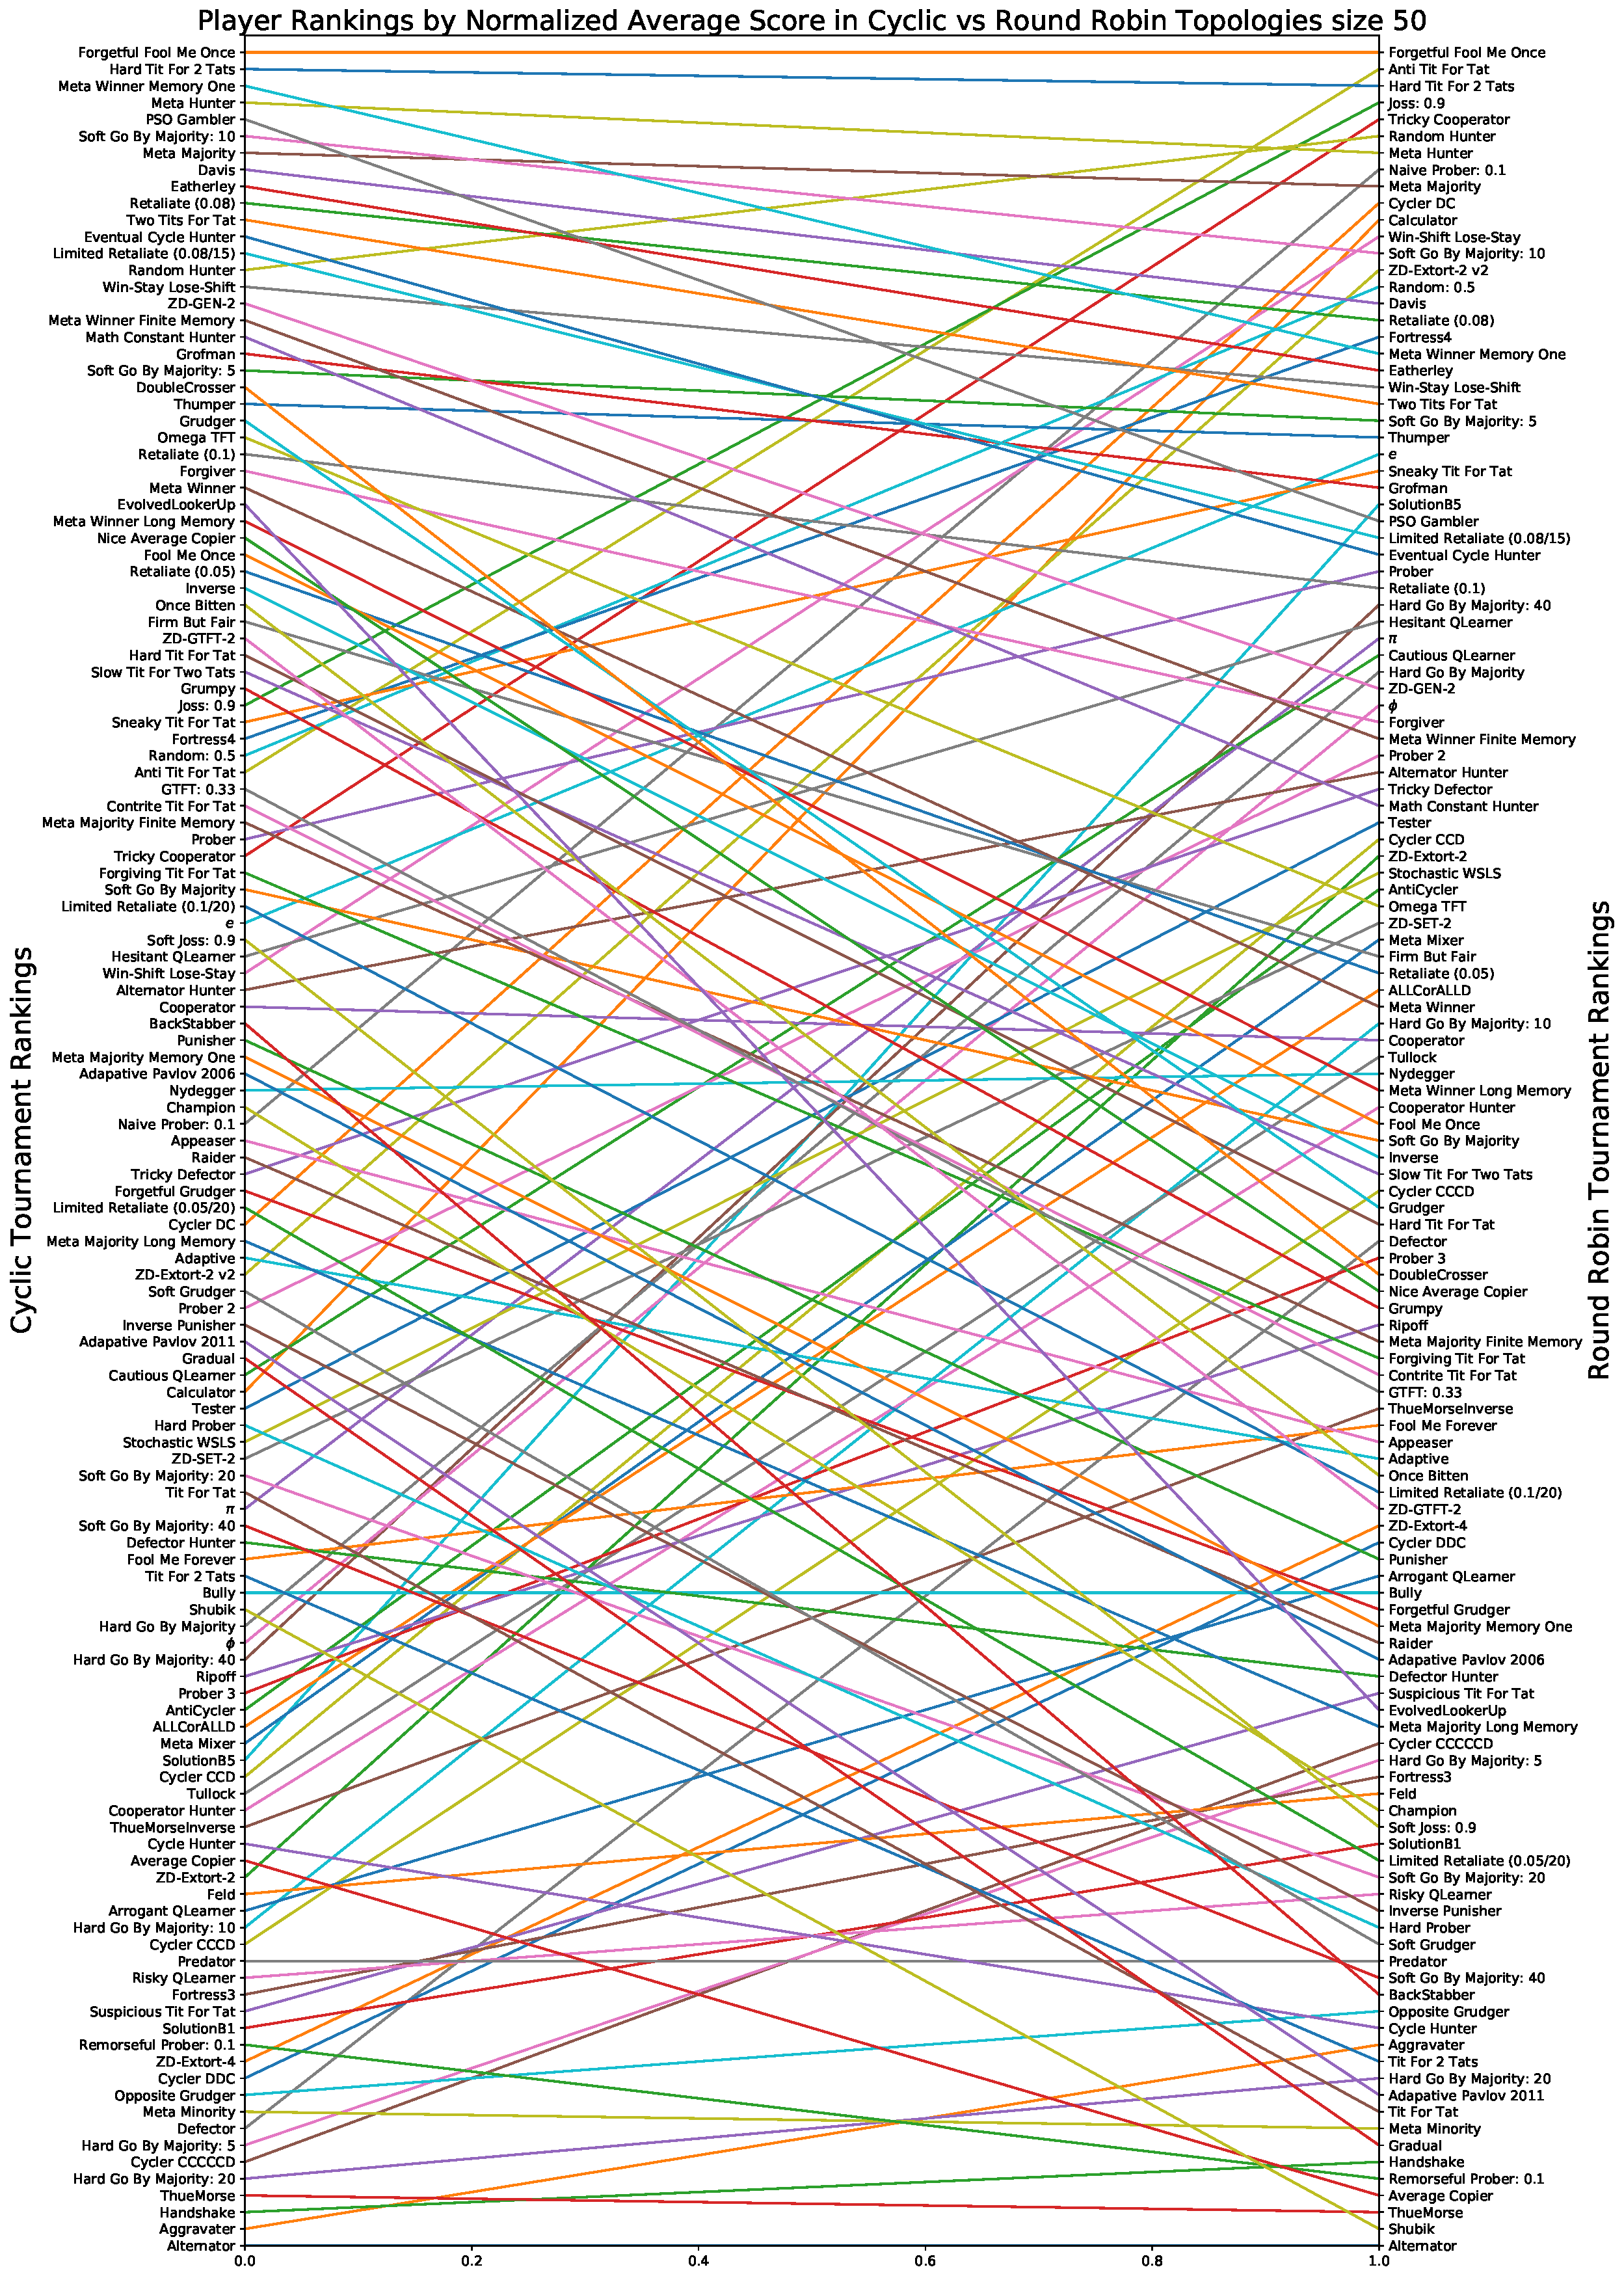
\includegraphics[width=\linewidth]{chapter-three/cyclic-round-robin-50.pdf}
	\caption{Cyclic vs Round Robin topologies size 50}
	\label{fig:score-rankings-fifty-c-r}
\end{figure}

\begin{figure}[H]
	\centering
	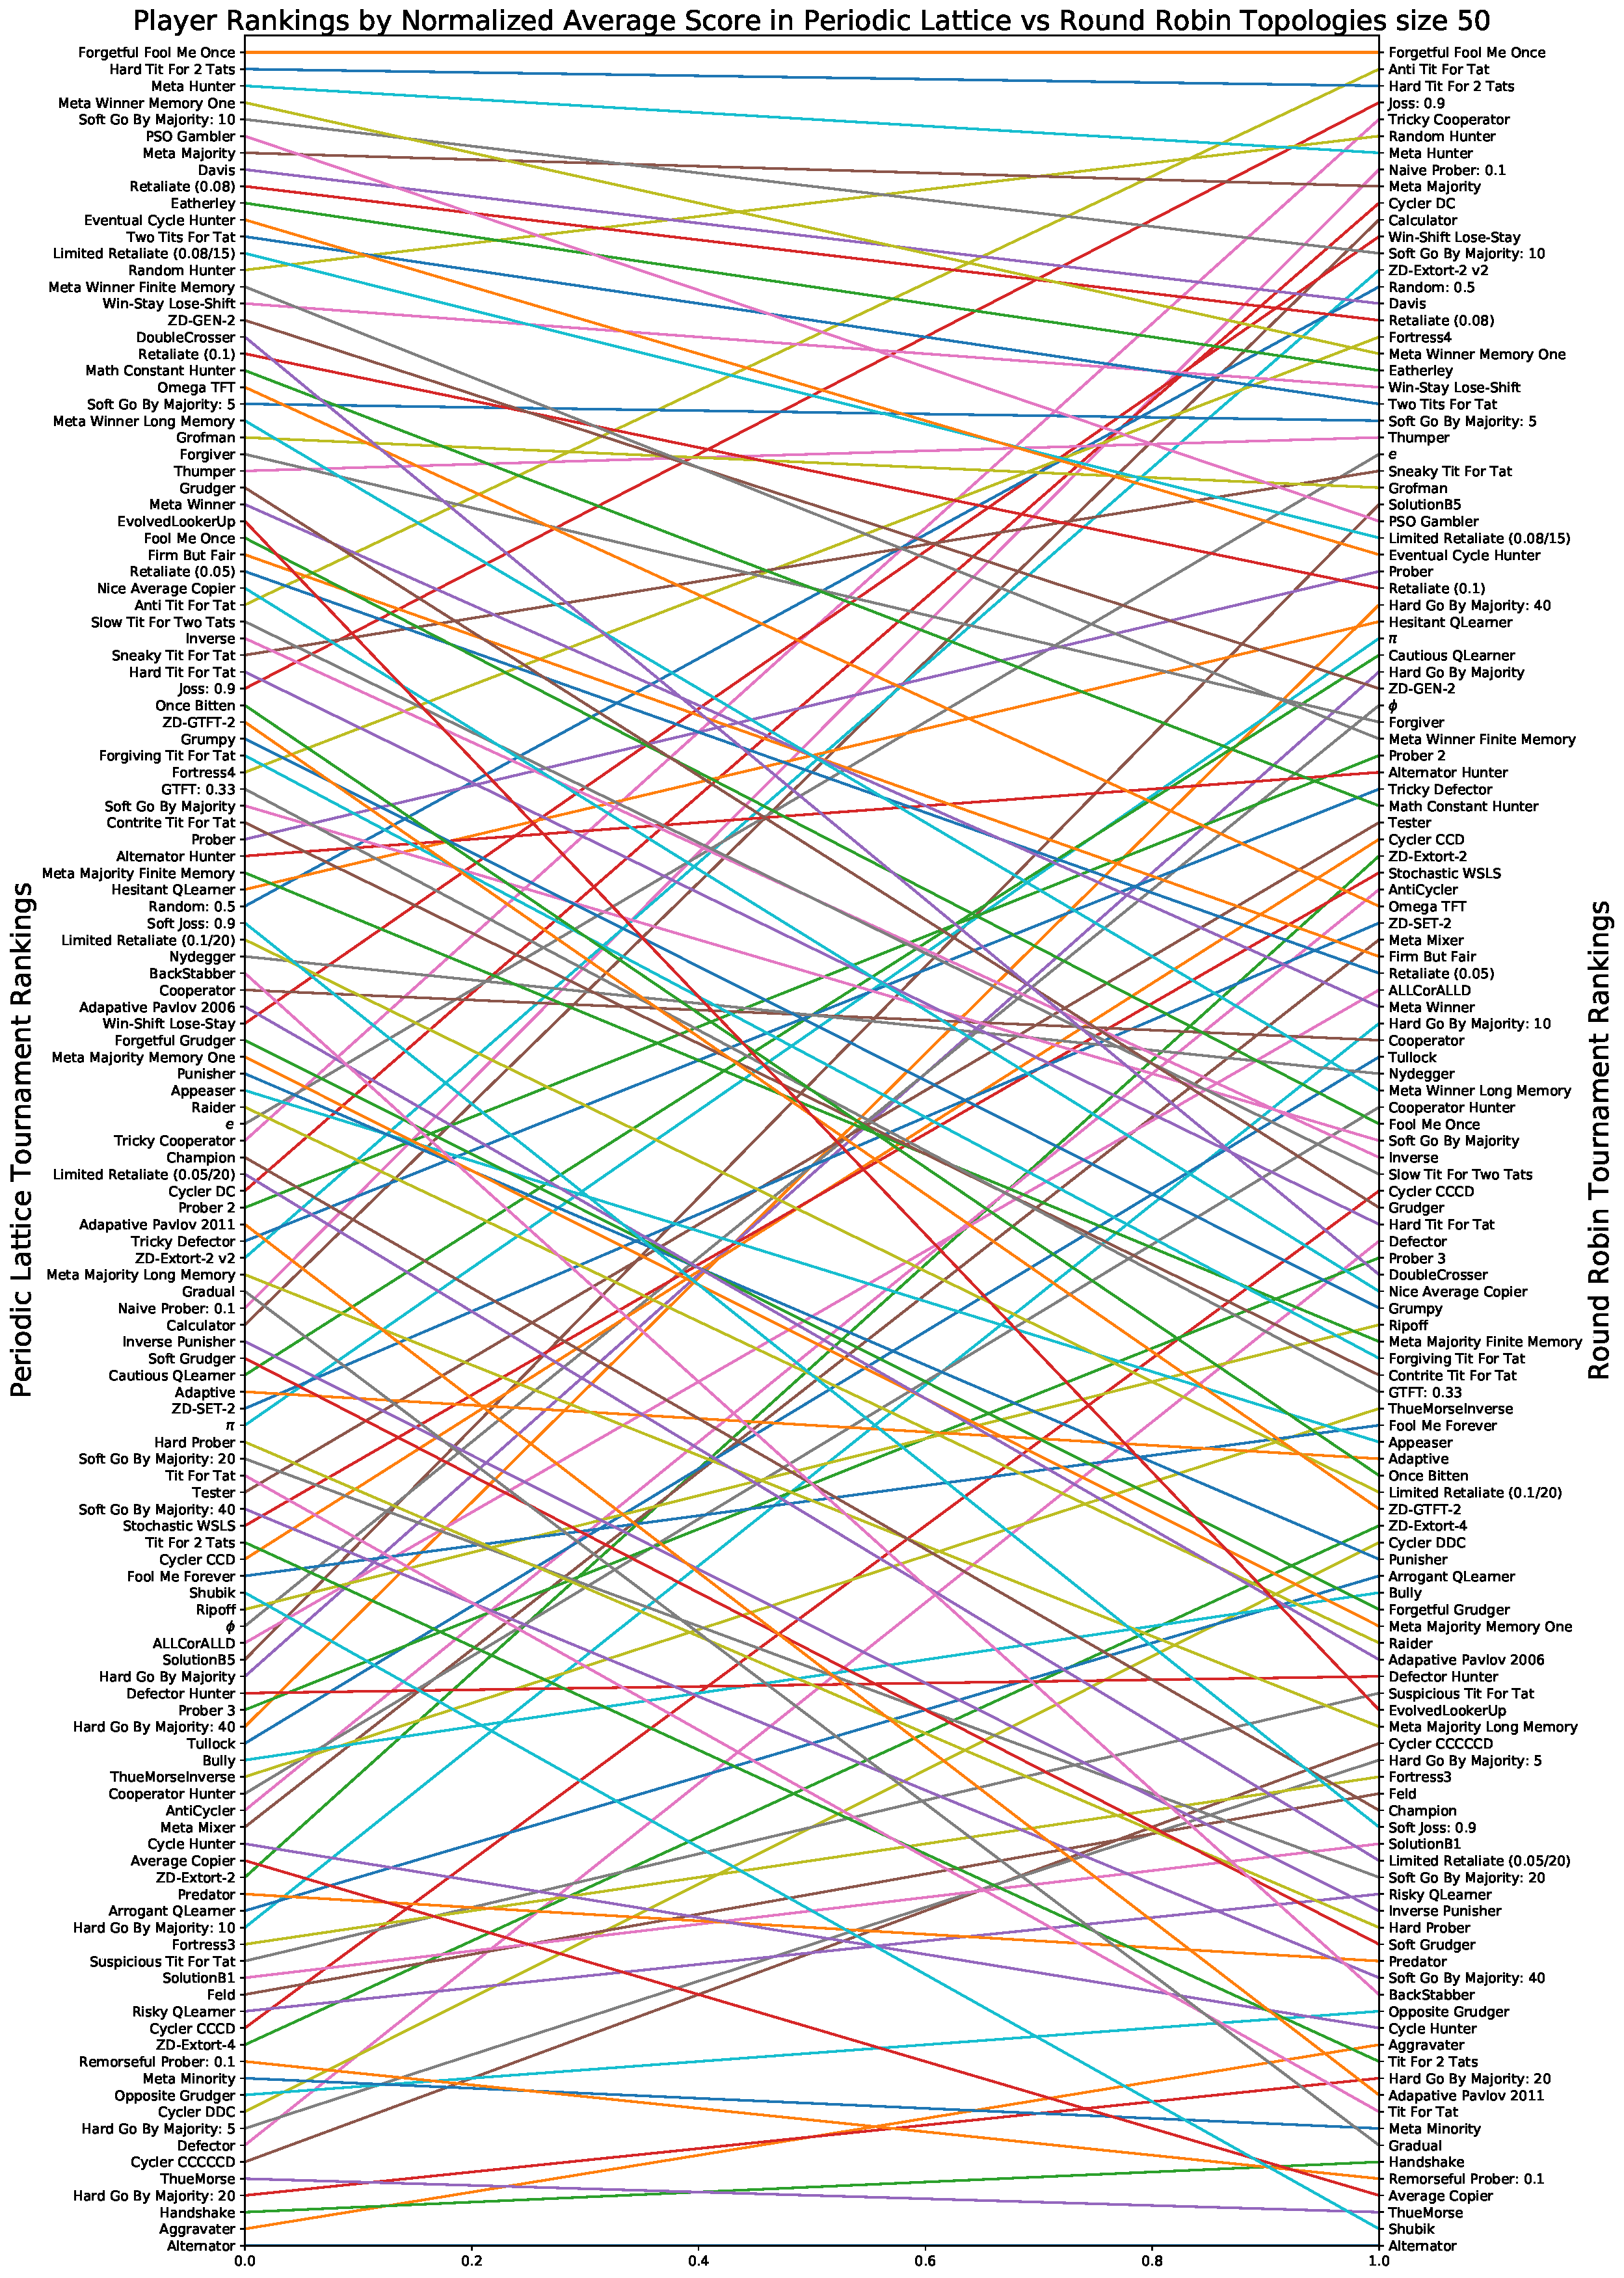
\includegraphics[width=\linewidth]{chapter-three/lattice-round-robin-50.pdf}
	\caption{Periodic Lattice vs Round Robin topologies size 50}
	\label{fig:score-rankings-fifty-l-r}
\end{figure}

Not many conclusions can be made out of this. The high variation could indicate
that the results are completely random. Unfortunately, this could mean that for
any random situation there does not seem to be a strategy that could
achieve a particularly high score although as described in~\autoref{sub:winning_ratio}
it is possible to ensure a good performance. Also, there has been difference in
the ranking, except for Raider. The conflict between the results of Tricky Cooperator and Hard Tit For 2 Tats,
give enough reasons to classify the wining ratio and  the normalized score as non satisfactory
measures. In the following subsection, a linear regression model is built as
considered to confirm and expand on these findings.

\subsection{Regression Analysis}
\label{sub:regression}
Finally, a common methodology when investing factors as predictors is building a
regression model~\cite{Bingham2010}. In this subsection two regression models are
used to identify any factors that can explain the winning ratio and average score
of a strategy. The round robin topology is not included in this subsection analysis
as this investigation aims to understand the effect of network topology.

The first model was built with the winning ratio as the depended variable,
shown here:

\begin{align}
	\mathrm{winning.ratio}_{t} = \alpha
	  & + \beta_{1}  \mathrm{degree}_{t}                              \\
	  & + \beta_{2}  \mathrm{average.neighborhood.score}_{t}          \\
	  & + \beta_{3}  \mathrm{clustering}_{t}                          \\
	  & + \beta_{4}  \mathrm{number.of.participations}_{t} + \epsilon
\end{align}

\begin{table}[!hbtp]
	\centering
	\begin{adjustbox}{width=1\textwidth, height=0.15\textwidth}
		\small
		\begin{tabular}{ccccccccccccc}
				\toprule
			Size 		& \multicolumn{1}{|l|}{Topology} & \multicolumn{2}{l|}{Intercept} & \multicolumn{2}{l|}{degree} & \multicolumn{2}{l|}{average neighborhood score} & \multicolumn{2}{l|}{clustering} & \multicolumn{2}{l|}{participations} & \(R\) square \\ \midrule
			        &         & coef   & \(p\)    & coef   & \(p\)    & coef       & \(p\)     & coef   & \(p\)    & coef       & \(p\)     &       \\ \midrule
			size 5  & Cyclic  & 0.0344 & 0.00 & 0.0688 & 0.00 & 3.239e-06  & 0.651 & 0.0    & NA   & 0.0006     & 0.00  & 0.007 \\ \midrule
			        & Lattice & 0.0108 & 0.00 & 0.0431 & 0.00 & 7.447e-06  & 0.159 & 0.0108 & 0.00 & -0.0002    & 0.036 & 0.001 \\ \midrule
			size 50 & Cyclic  & 0.0043 & 0.00 & 0.0087 & 0.00 & -1.386e-06 & 0.00  & 0      & NA   & -8.156e-07 & 0.216 & 0.002 \\ \midrule
			        & Lattice & 0.0008 & 0.00 & 0.0031 & 0.00 & -4.549e-07 & 0.00  & 0.0004 & 0.00 & 2.005e-05  & 0.00  & 0.022 \\ \bottomrule
		\end{tabular}
	\end{adjustbox}
	\caption{Regression results for winning ratio model}
	\label{regression-winning}
\end{table}

For tournaments of size 50, the results show that only the degree seems
to be a stable significant predictor for all two experiments. With a \(p\)
value less that 0.001. Average neighborhood score, has a negative correlation
with the winning ratio. Thus, the better the neighbors score the
less score a strategy will achieve, indicating beneficial uncooperative behavior.

Periodic lattice experiments are affected by clustering. Both \(p\) values
are less than 0.05 but are affected with an insignificant amount, less that 0.1.
Participations seems to have a negative effect on the lattice size 5 experiment
but a positive one for the cyclic size 5 and lattice size 50.

Overall, all \(R\) square values  are really low. With the highest value of
\(R\) square being 0.022 for lattice size 50. Thus, the performance of the
model can be characterized as insignificant,

The second model using the normalized average score is the following.

\begin{align}
	\mathrm{average.normalised.score}_{t} = \alpha
	  & + \beta_{1}  \mathrm{degree}_{t}                              \\
	  & + \beta_{2}  \mathrm{average.neighborhood.score}_{t}          \\
	  & + \beta_{3}  \mathrm{clustering}_{t}                          \\
	  & + \beta_{4}  \mathrm{number.of.participations}_{t} + \epsilon
\end{align}

The model was used to each of the experiments for lattice and cycle topologies
individually. The results of models are shown below, Table~\ref{regression-average} :

\begin{table}[H]
	\centering
	\begin{adjustbox}{width=1\textwidth, height=0.15\textwidth}
		\small
		\begin{tabular}{ccccccccccccc}
				\toprule
			Size 		& \multicolumn{1}{|l|}{Topology} & \multicolumn{2}{l|}{Intercept} & \multicolumn{2}{l|}{degree} & \multicolumn{2}{l|}{average neighborhood score} & \multicolumn{2}{l|}{clustering} & \multicolumn{2}{l|}{participations} & \(R\) square \\ \midrule
			        &         & coef   & \(p\)    & coef   & \(p\)    & coef       & \(p\)     & coef   & \(p\)    & coef       & \(p\)     &       \\ \midrule
			size 5  & Cyclic  & 0.028  & 0.00 & 0.0559 & 0.00 & -3.763e-06 & 0.043 & 0.0    & NA   & -0.0016    & 0.00 & 0.457 \\ \midrule
			        & Lattice & 0.0064 & 0.00 & 0.0256 & 0.00 & 1.079e-05  & 0.00  & 0.0064 & 0.00 & -0.0016    & 0.00 & 0.549 \\ \midrule
			size 50 & Cyclic  & 0.0025 & 0.00 & 0.0051 & 0.00 & -2.168e-07 & 0.00  & 0      & NA   & -1.602e-05 & 0.00 & 0.120 \\ \midrule
			        & Lattice & 0.0006 & 0.00 & 0.0024 & 0.00 & 1.033e-06  & 0.00  & 0.0003 & 0.00 & -1.601e-05 & 0.00 & 0.216 \\ \bottomrule
		\end{tabular}
	\end{adjustbox}
	\caption{Regression results for average score model}
	\label{regression-average}
\end{table}

In the output, Table~\ref{regression-average}, is shown that degree, average
neighborhood score and participations
are significant predictors for all the experiments with a \(p\) value less than
an 0.0001.
For the cyclic topology, average neighborhood score and participations have negative
coefficient. For example a decrease in participations by one would increase
the average score by 0.0016. Degree on the other hand has a positive coefficient
and connectivity has no effect at all. Furthermore the model for size 5 has
a \(R\) square value of 0.457, thus it only explains 0.4 variation of the data which is
quite low. For size 50 it is even lower at only 0.12.

Finally, for the lattice topology only participations have a negative coefficient.
Thus the only factor with a reverse influence on average score in the lattice topology.
Connectivity is a significant predictor as well with a coefficient 0.0064 and
0.0003 respectively. Though the \(R\) square value is still  small,
with a value 0.547 and 0.216 respectively.
Even if there are predictors with a significant \(p\) value, the overall
performance of the model is moderate.

For both models and all set of 6 experiments some predictors can be characterized
as significant. More than one factors have a \(p\) value less than a 0.05, the \(alpha\)
that has been set. Even so, the coefficient and the overall \(R\) square values are
quite low. This in fact indicates
that none of the characteristics of the networks seem to have an effect on
performance. This is potentially expected due to the simplistic nature of the
topologies considered which in effect (when repeated sampling is considered)
correspond to randomly matching up strategies.


\section{Summary}
\label{sub:summary}
A summary of all the analysis previously made, ~\autoref{sub:intro-three} and
~\autoref{sub:analyzing_the_effect_of_the_topologies}, is given in this section.
Moreover, it lists topic for further research to be conducted.

In this chapter, it has been explained how the concept of spatial tournaments,
has been produced, by adding to an already existed the Axelrod-Python library.
Secondly, an experiment using the new capabilities of the library has been
conducted. In this experiment, some of the most common topologies have been used.
They have been presented and analyzed, as well as the structure of the experiments.

An initial analysis for the data, created from the experiment, was carried out.
Followed by, an analysis for the results of the games themselves.
Two measures have been used, the wining ratio and the normalized score. The
wining ratio returned, that the following strategies have outperformed the rest.
Raider, Backstabber and PSO Gambler. As for the normalized score, it indicated
that Tricky Cooperator,  Raider, Hard Tit For 2 Tats and Fool Me Once, have been the
highest ranked strategies. Even if, Raider has been repeating, strategies like
Tricky Cooperator have been ranked completely differently by the two measures.
Creating a conflict and indicating that these measures are perhaps not adequate
(this will be expanded on in~\autoref{chap:Four}).

An attempt to find any significant reason as to why these strategies outperform
the rest gave the findings below:

\begin{itemize}
	\item Winning ratio has a significant difference based on the participations
	      number only for the cyclic and lattice topologies of size 5.
	\item There is high variation in the average score of each strategy for all
	      experiments.
	\item Both regression models for the winning ratio and the normalized average
	      score returned that significantly there was no significant effect.
\end{itemize}

Comparing the results to any other work done in the literature is not possible.
Because this kind of experiments (which compare a large number of tournaments)
have not been conducted before.
The Axelrod-Python library tournament could be used  a measure of comparison.
Still two (PSO Gambler, BackStabber) of the best overall strategies of that
tournament have only made a brief appearance.

Further actions to the experiments and can be taken for this point on.
Producing a more complete data set for each experiment and carrying out a more
in depth analysis. One could argue that all above experiments
were conducted in simple topologies and a small number of repetitions. Thus, the
next step is to use more complex networks for topologies and conduct a larger
number of tournaments.
